\documentclass[letter]{article}

\usepackage{fullpage}
\usepackage{url}

\title{Performance investigation}

\usepackage[pdftex]{graphicx}
\usepackage{multirow}
\usepackage{caption}
\usepackage{subcaption}
\usepackage{float}

%\usepackage[top=0.75in, bottom=0.75in, left=1in, right=1in]{geometry}

\begin{document}
\maketitle

\section{Constant ratio between sources/destinations =  1/8}

\subsection{Disjoint set - Test Id = 3}

Among N nodes, N/2 source nodes send data to N/16 destination nodes. The destination nodes are among the source nodes. There are N/2 pairs of communication, 8 MB of data per pair. There is 1 MPI/PAMI rank per node. Experiments are done for N=512, 1024, 2048, 4096 and 8192 nodes.

\begin{figure}[h]
\vspace{-0.1in}
\centering
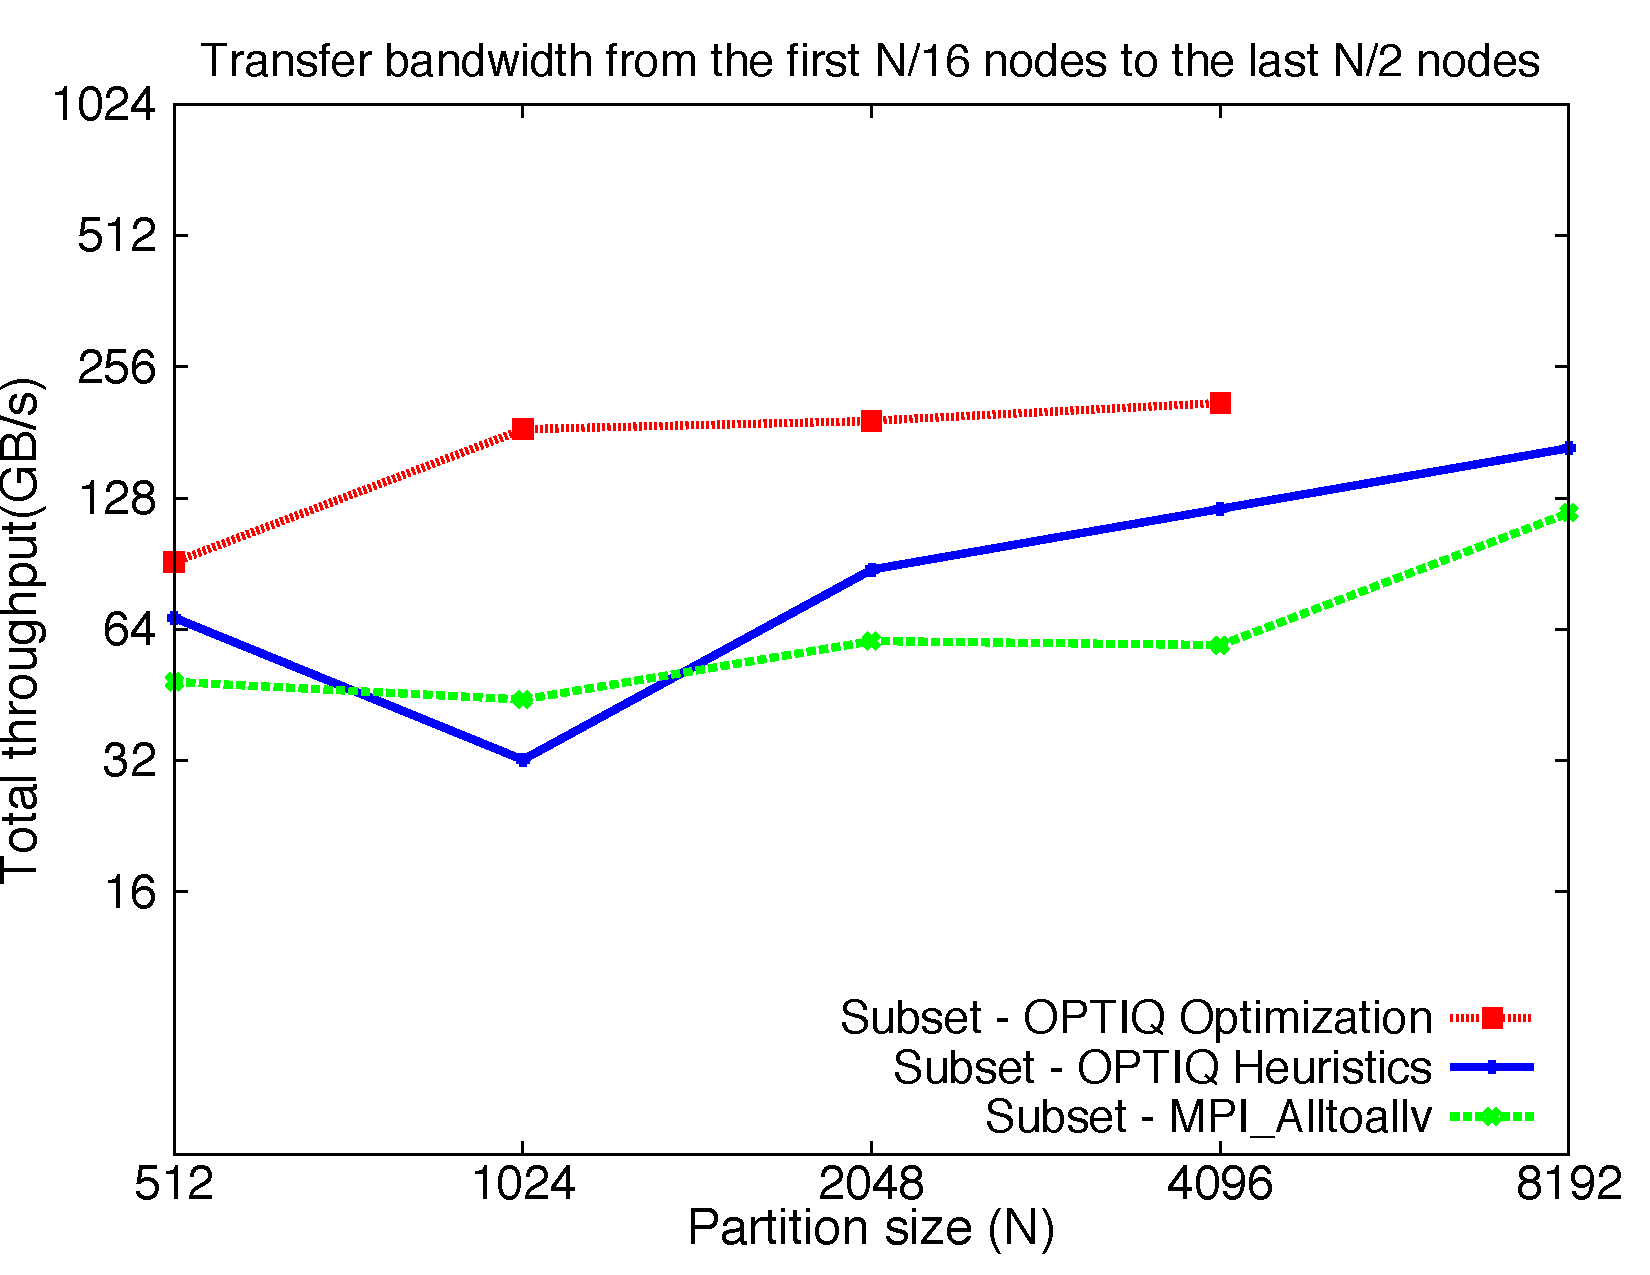
\includegraphics[scale=0.40]{report_figures/constantr_3.pdf}
\vspace{-0.1in}
\caption{Disjoint performance}
\vspace{-0.1in}
\label{fig:patterns}
\end{figure}

\newpage

\subsubsection{Number of nodes 512}

\input{tables/tables_3_512.dat}

\begin{figure}[!htbp]
        \centering
        \begin{subfigure}[b]{0.49\textwidth}
                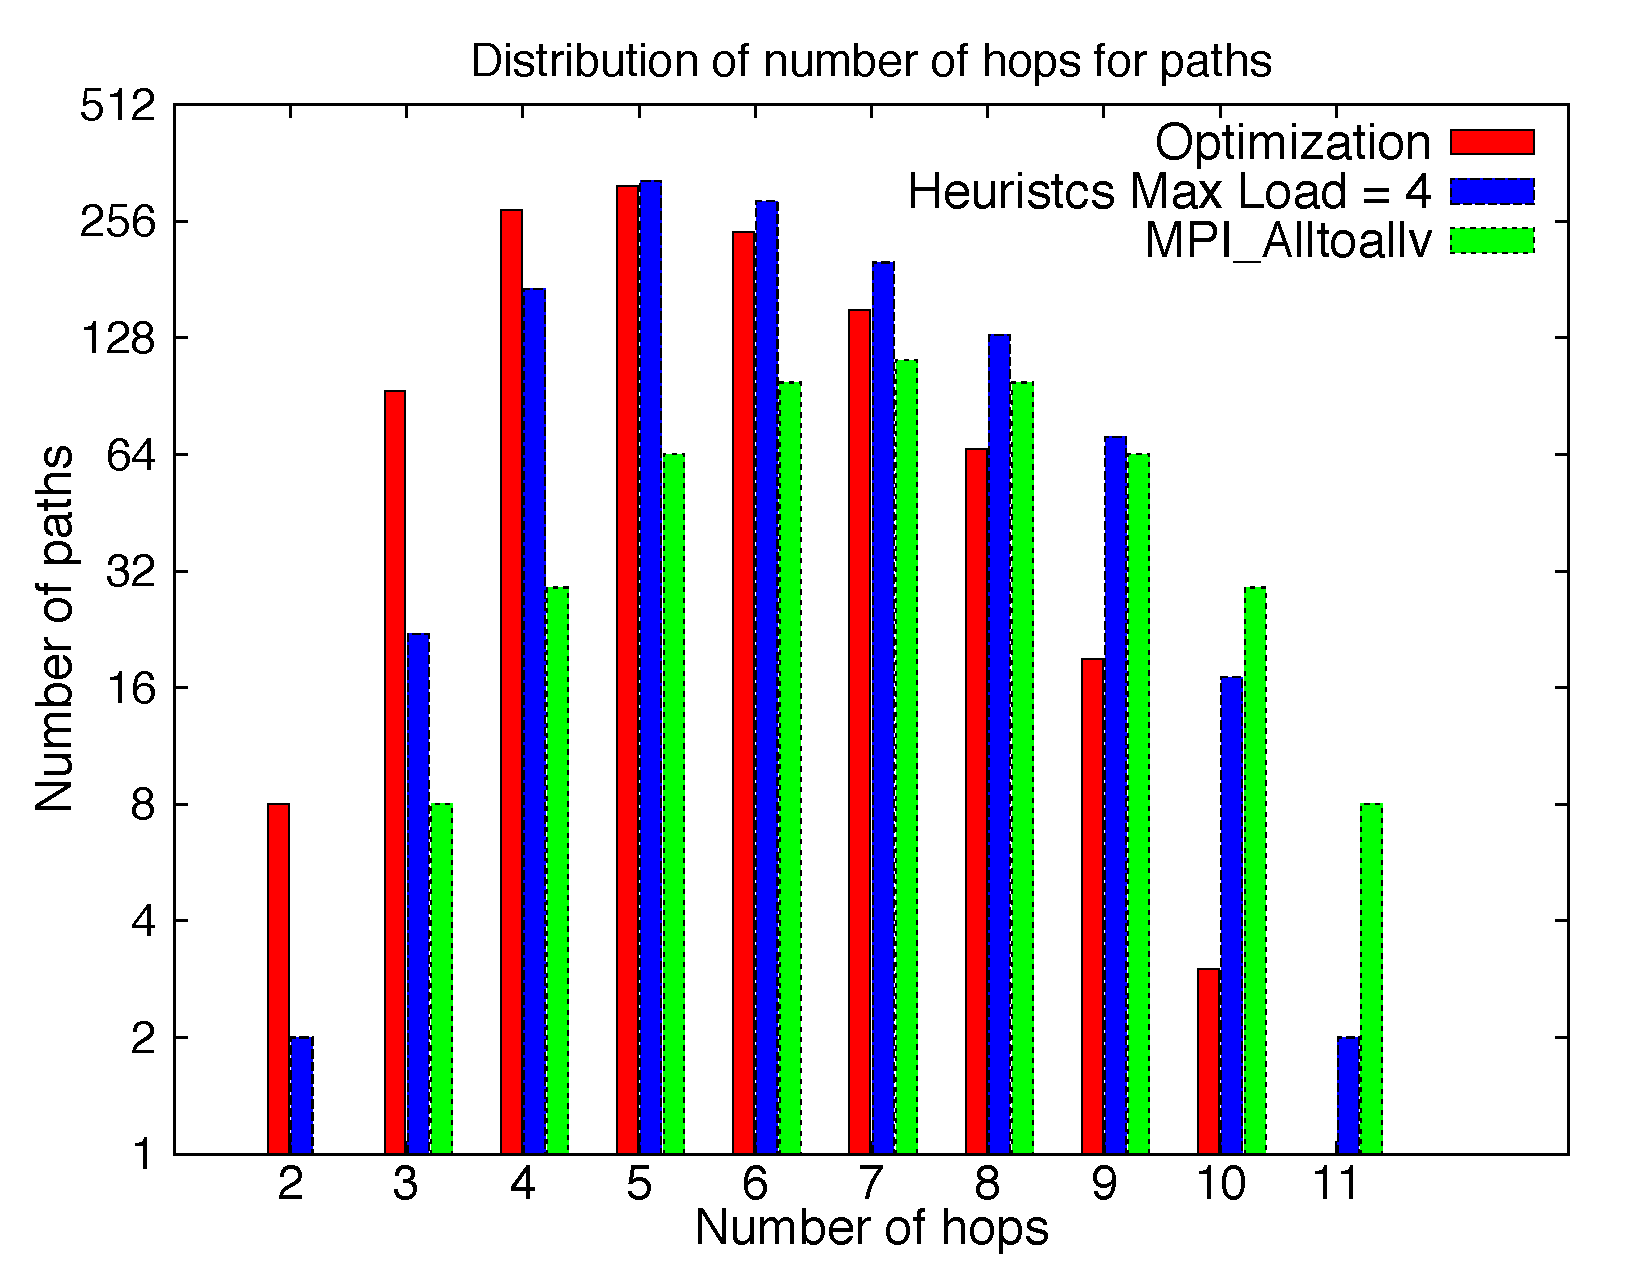
\includegraphics[width=\textwidth]{report_figures/constantr/3_1024/hop_histo.pdf}
                \caption{Distribution of number of hops over paths}
                \label{fig:3_1024_hop}
        \end{subfigure}%
        ~ %add desired spacing between images, e. g. ~, \quad, \qquad, \hfill etc.
          %(or a blank line to force the subfigure onto a new line)
        \begin{subfigure}[b]{0.49\textwidth}
                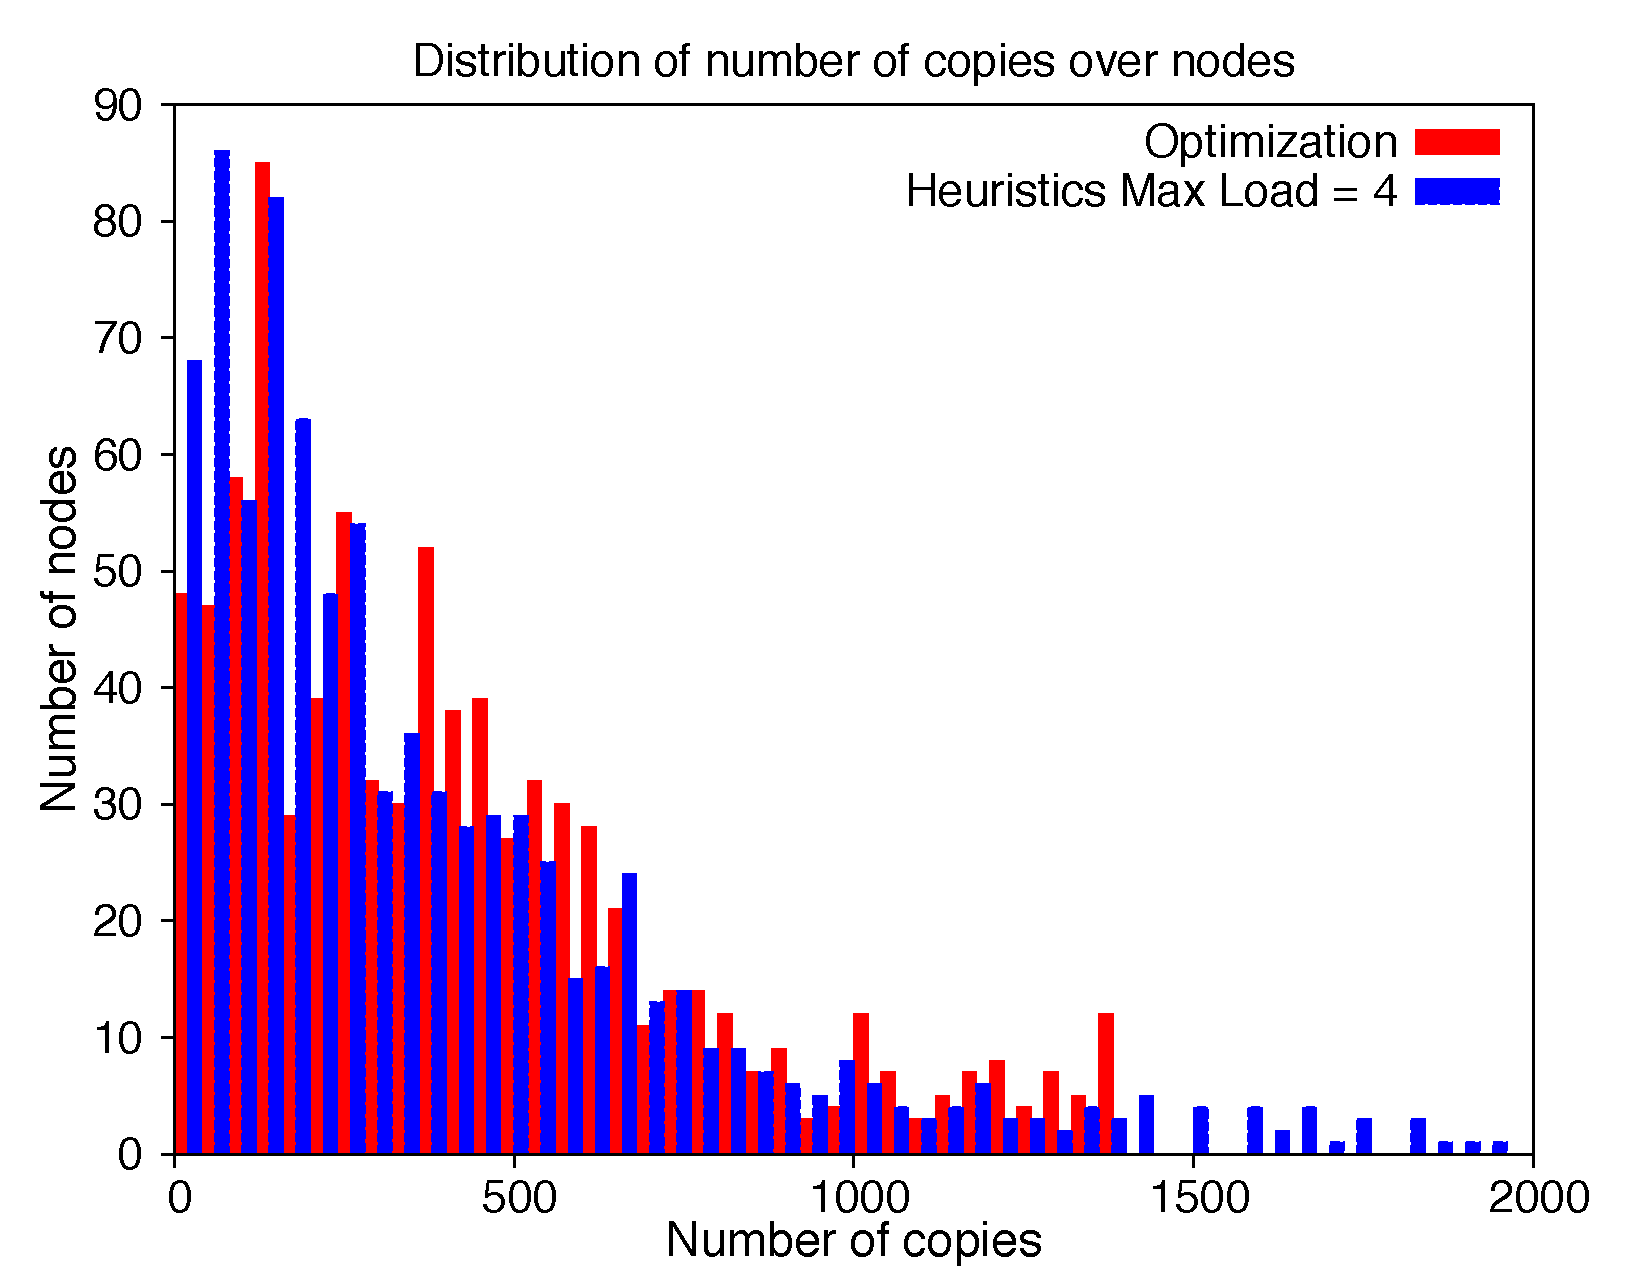
\includegraphics[width=\textwidth]{report_figures/constantr/3_1024/copy_histo.pdf}
                \caption{Distribution of number of copies over nodes}
                \label{fig:3_1024_copy}
        \end{subfigure}
        ~ %add desired spacing between images, e. g. ~, \quad, \qquad, \hfill etc.
          %(or a blank line to force the subfigure onto a new line)
        \begin{subfigure}[b]{0.49\textwidth}
                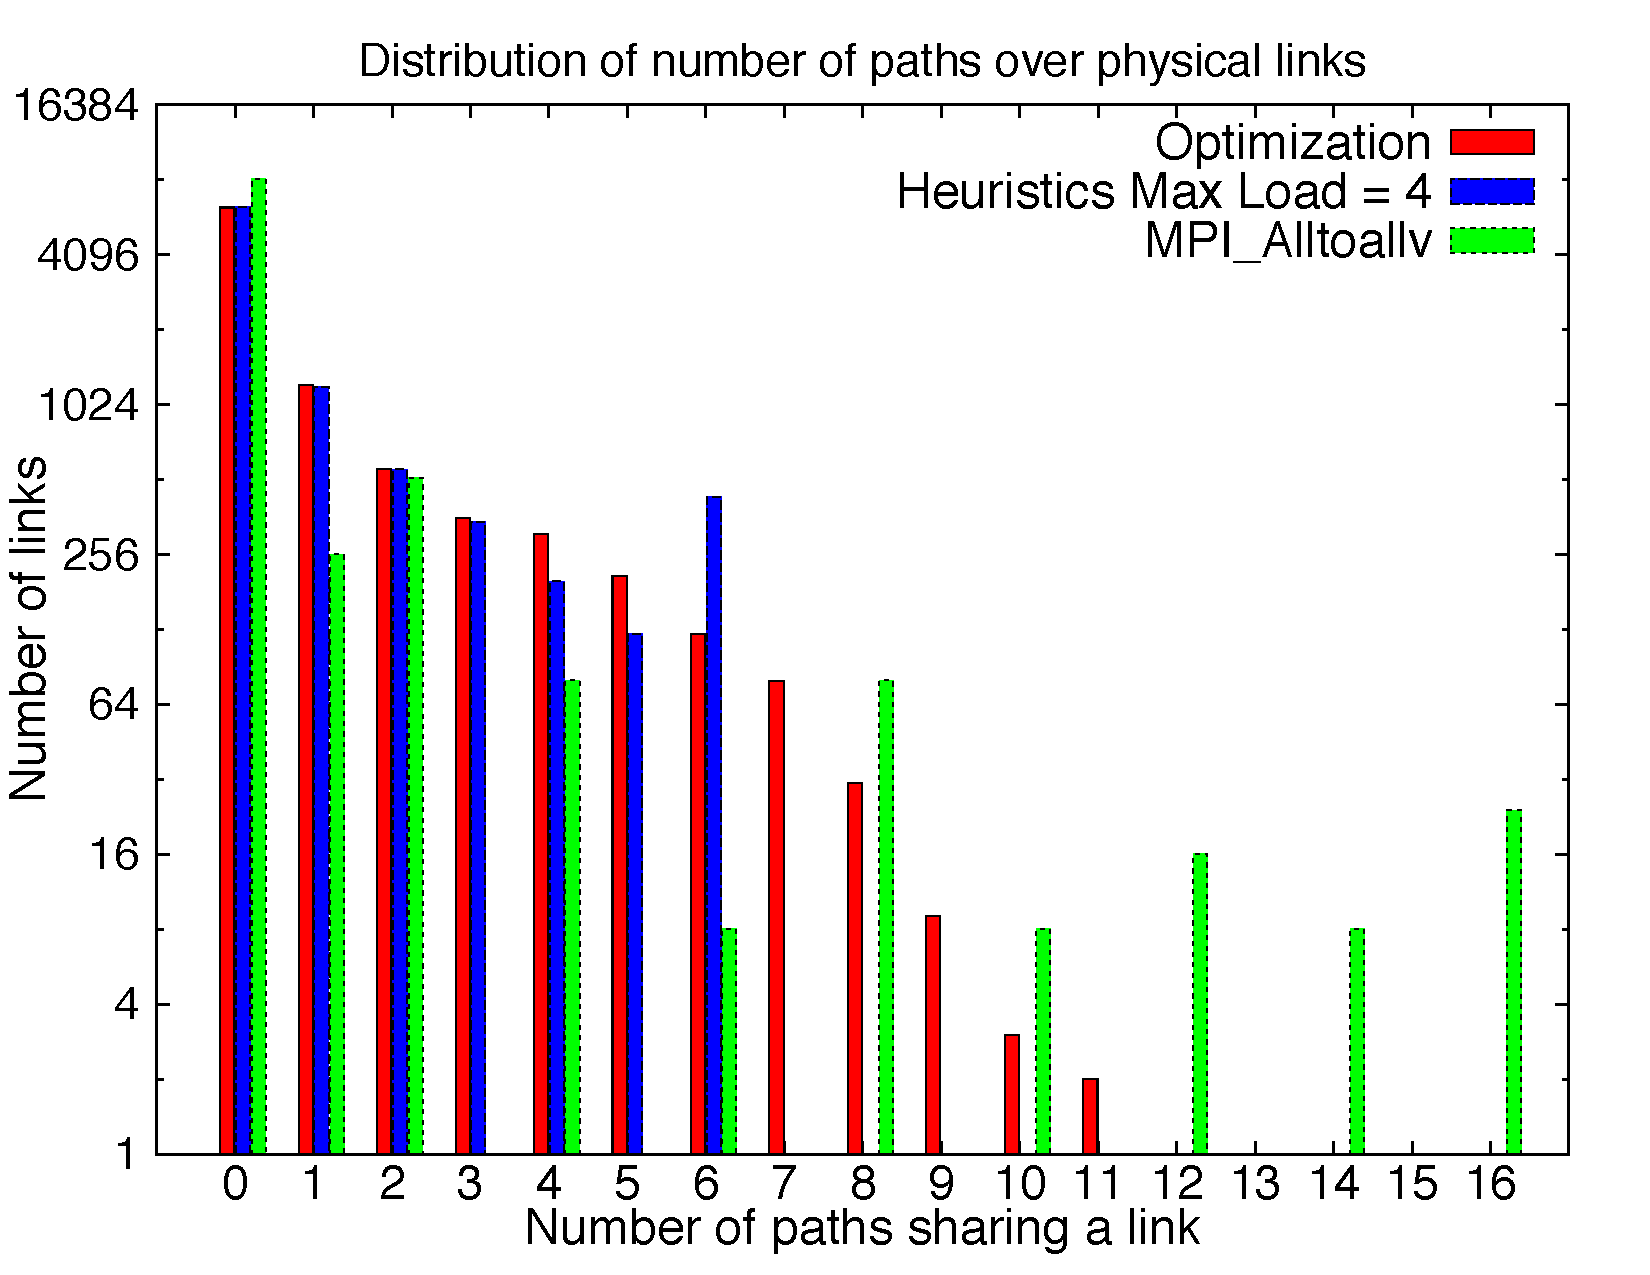
\includegraphics[width=\textwidth]{report_figures/constantr/3_1024/loadpath_histo.pdf}
                \caption{Distribution of number of paths over physicallinks}
                \label{fig:3_1024_loadpath}
        \end{subfigure}
        ~ %add desired spacing between images, e. g. ~, \quad, \qquad, \hfill etc.
          %(or a blank line to force the subfigure onto a new line)
        \begin{subfigure}[b]{0.49\textwidth}
                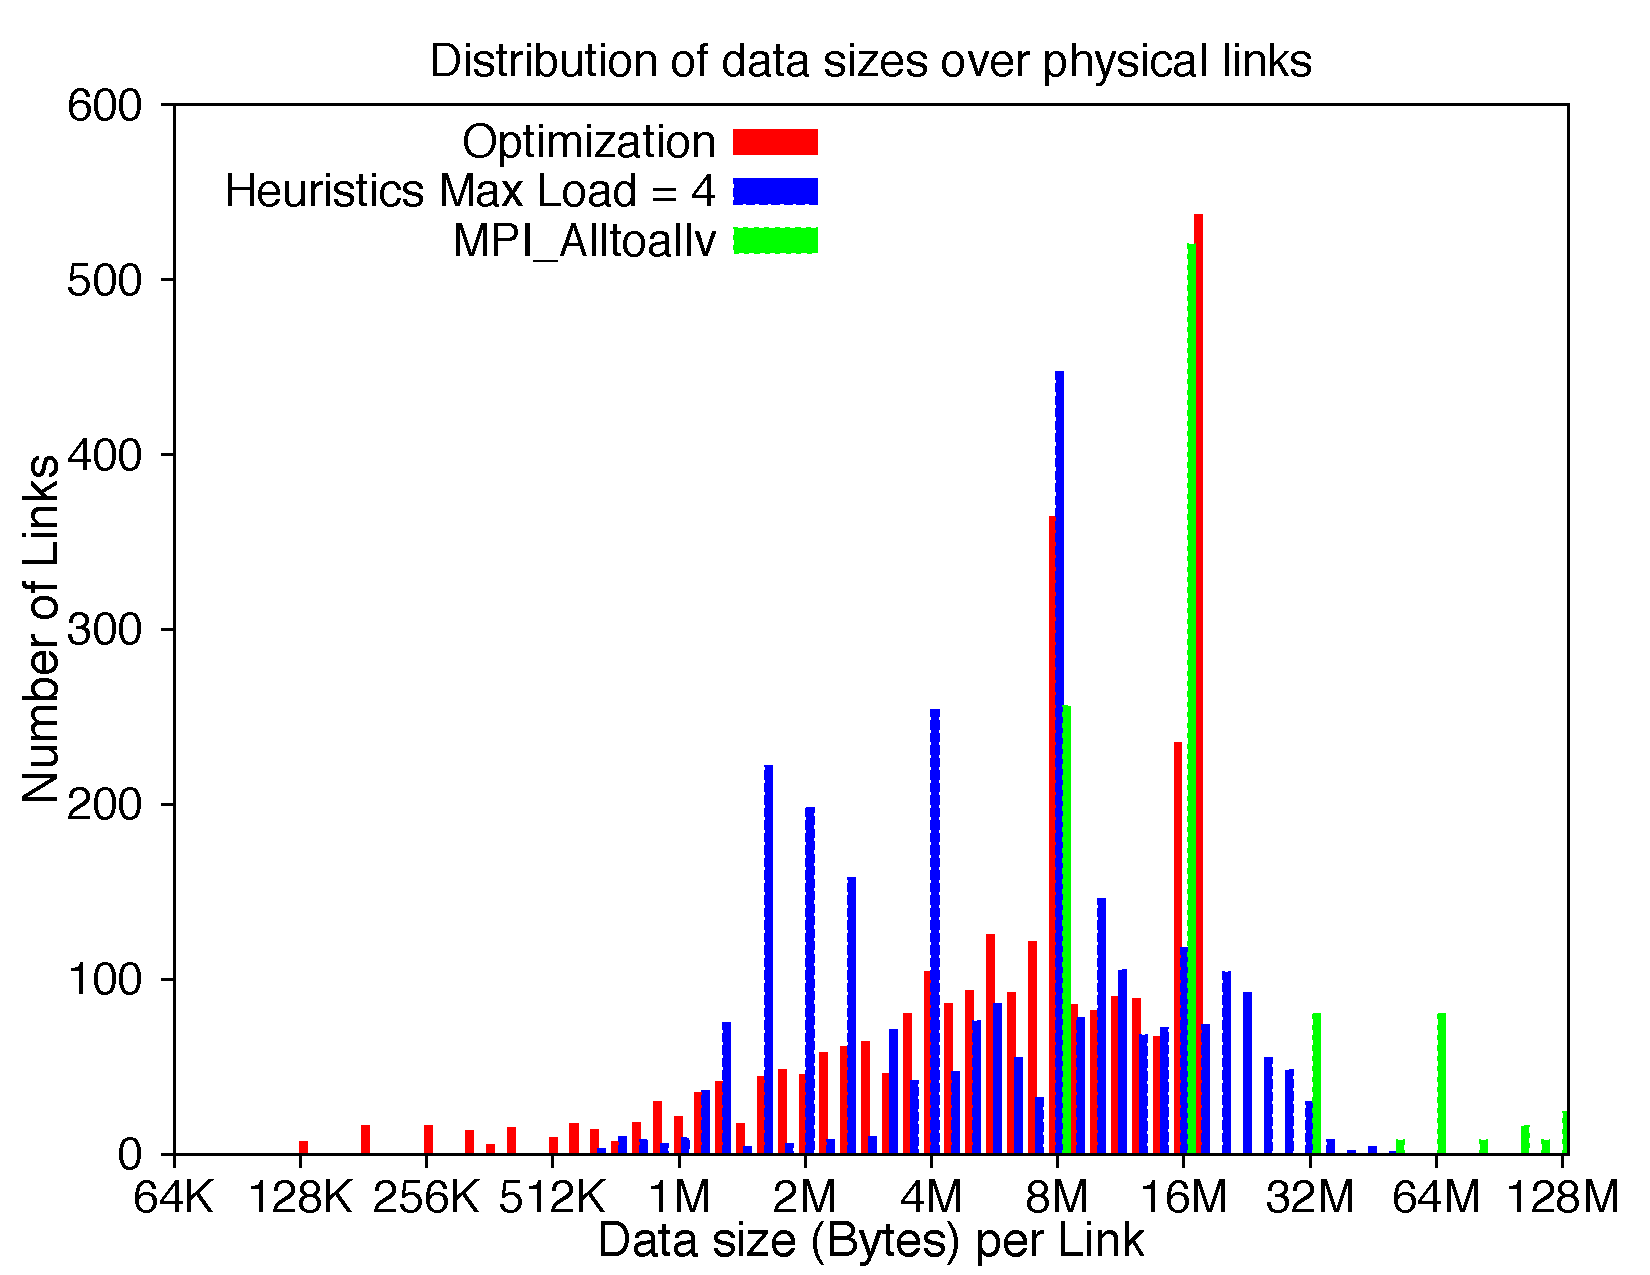
\includegraphics[width=\textwidth]{report_figures/constantr/3_1024/loaddata_histo.pdf}
                \caption{Distribution of total data size over physical links}
                \label{fig:3_1024_loaddata}
        \end{subfigure}
        ~ %add desired spacing between images, e. g. ~, \quad, \qquad, \hfill etc.
          %(or a blank line to force the subfigure onto a new line)
        \begin{subfigure}[b]{0.49\textwidth}
                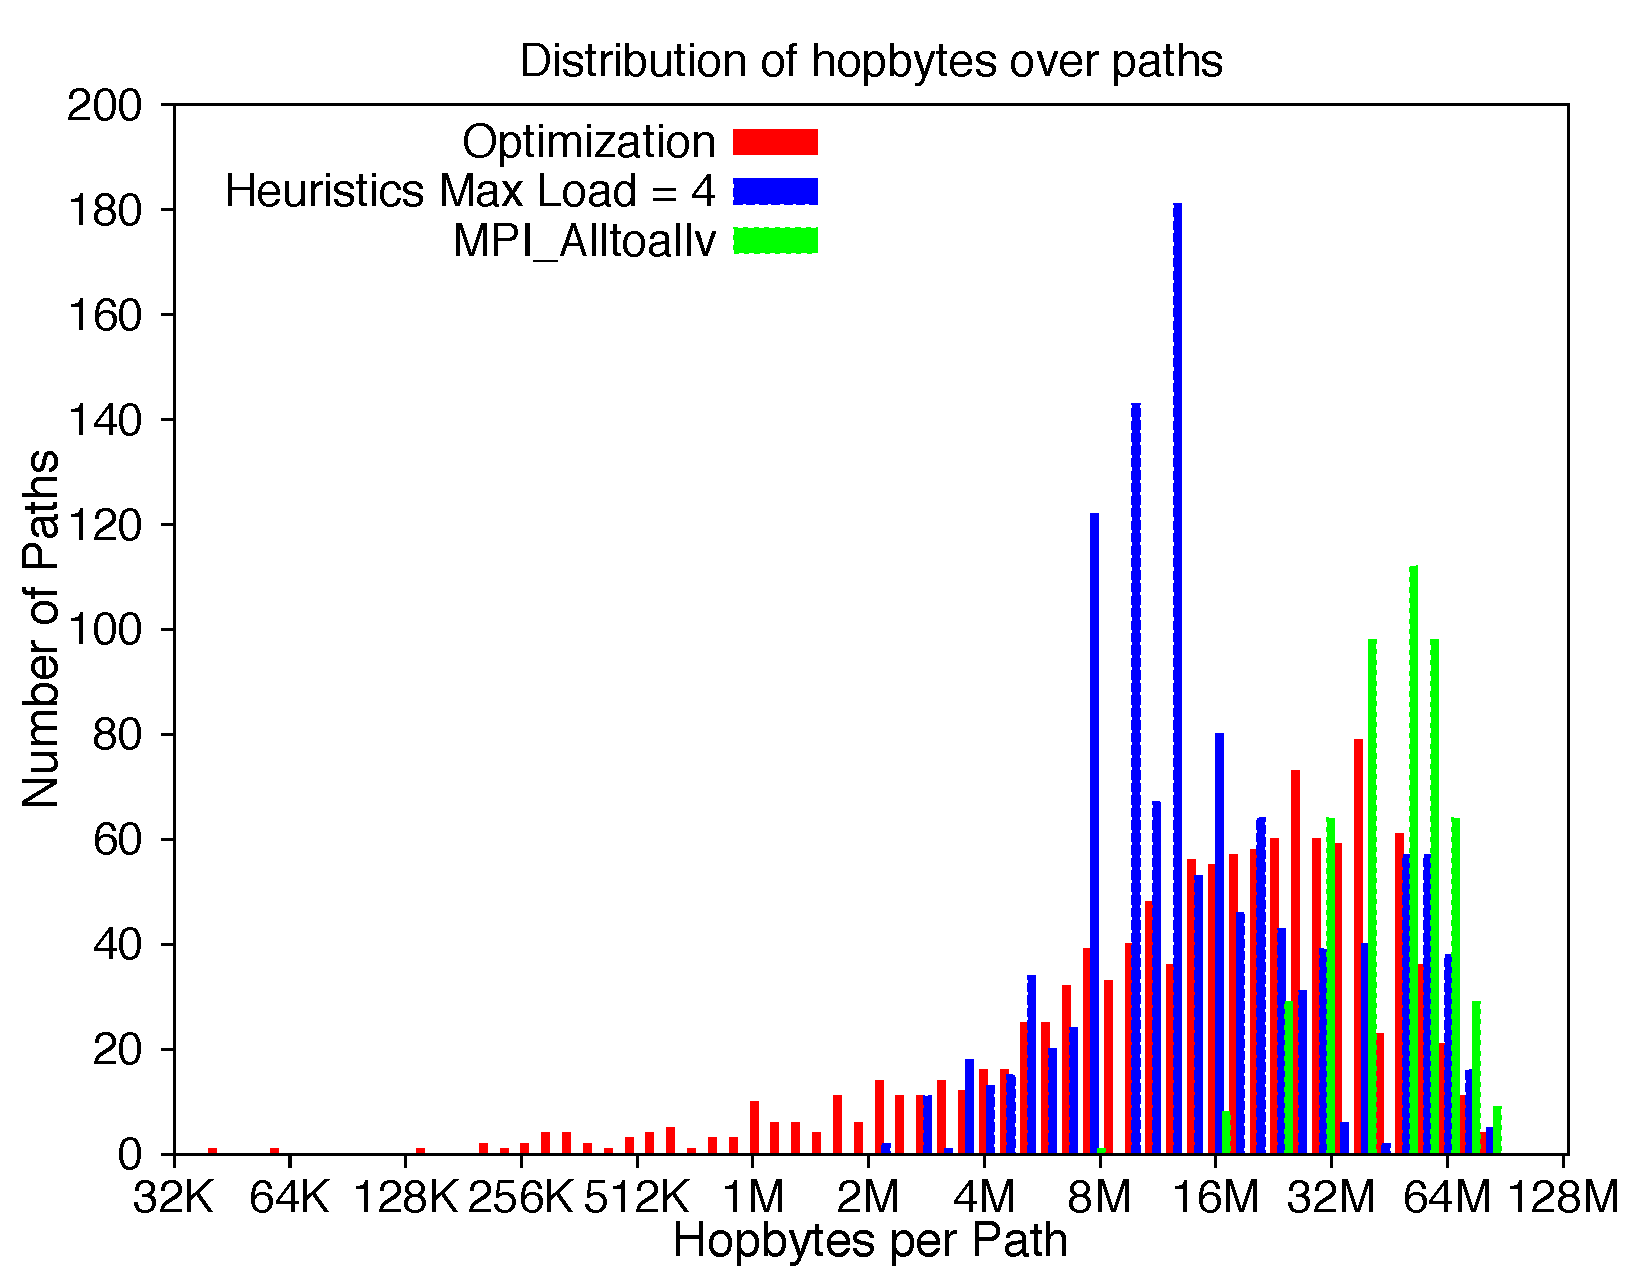
\includegraphics[width=\textwidth]{report_figures/constantr/3_1024/hopbyte_histo.pdf}
                \caption{Distribution of hopbytes over paths}
                \label{fig:3_1024_hopbyte}
        \end{subfigure}
        ~ %add desired spacing between images, e. g. ~, \quad, \qquad, \hfill etc.
          %(or a blank line to force the subfigure onto a new line)
        \begin{subfigure}[b]{0.49\textwidth}
                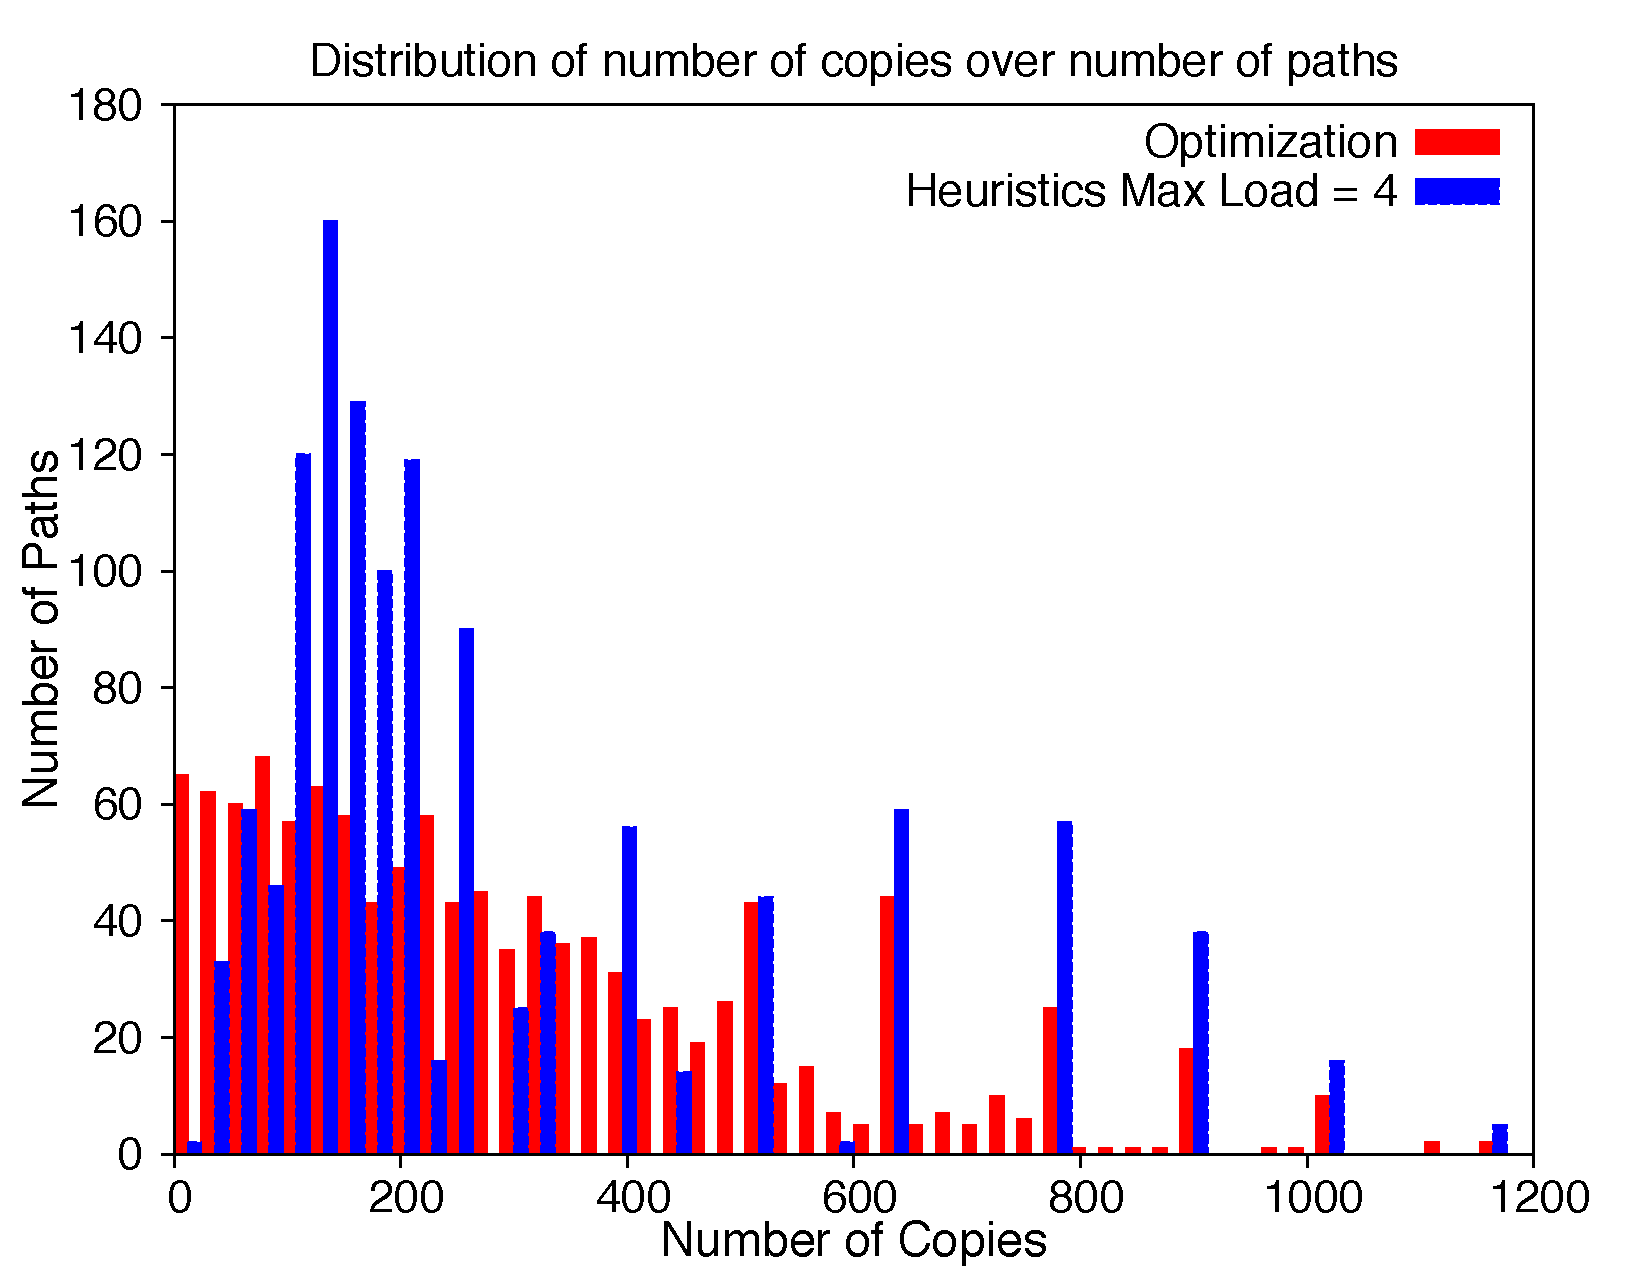
\includegraphics[width=\textwidth]{report_figures/constantr/3_1024/hopcopy_histo.pdf}
                \caption{Distribution of number of copies over paths}
                \label{fig:3_1024_hopcopy}
        \end{subfigure}
        \caption{Historgram of hops, copies, load in terms of number of paths and data size}
        \label{fig:3_1024_histo}
\end{figure}



\newpage

\subsubsection{Number of nodes 1024}

\input{tables/tables_3_1024.dat}

\begin{figure}[!htbp]
        \centering
        \begin{subfigure}[b]{0.49\textwidth}
                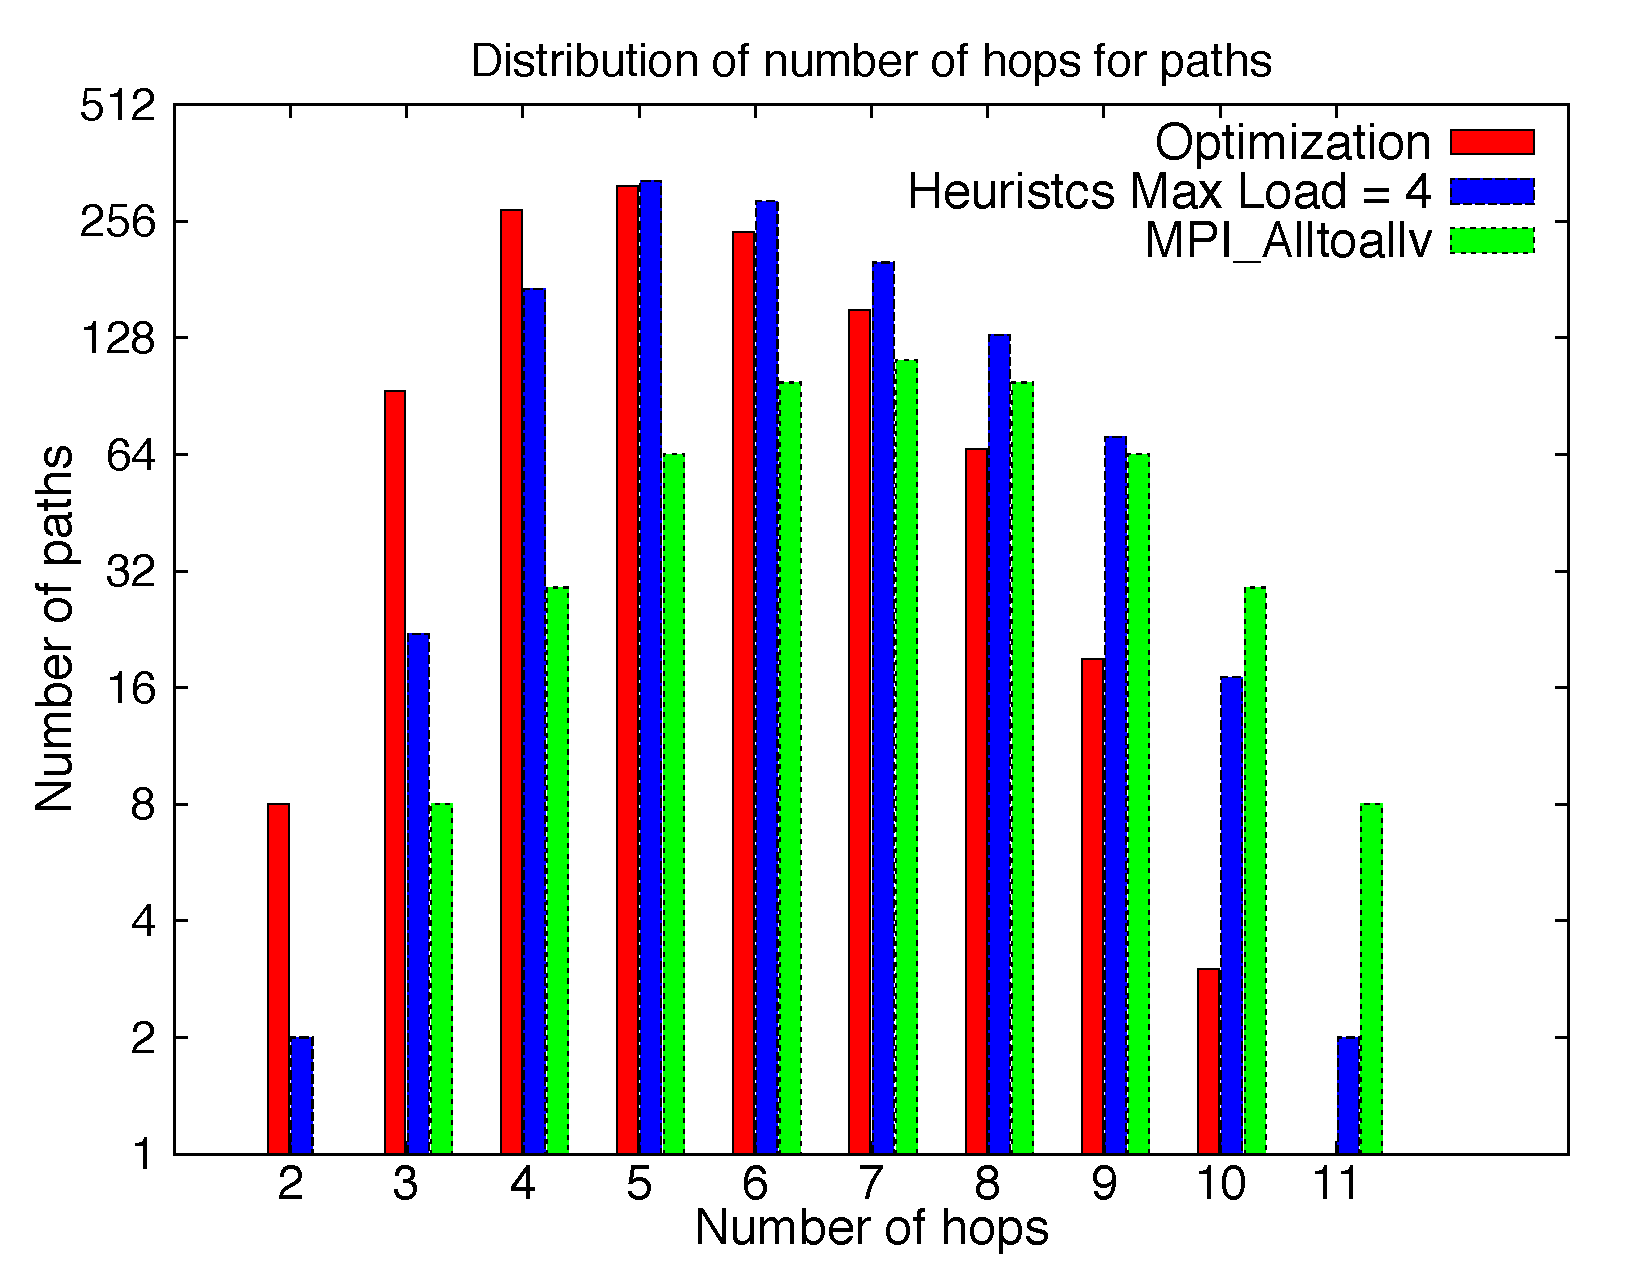
\includegraphics[width=\textwidth]{report_figures/constantr/3_1024/hop_histo.pdf}
                \caption{Distribution of number of hops over paths}
                \label{fig:3_1024_hop}
        \end{subfigure}%
        ~ %add desired spacing between images, e. g. ~, \quad, \qquad, \hfill etc.
          %(or a blank line to force the subfigure onto a new line)
        \begin{subfigure}[b]{0.49\textwidth}
                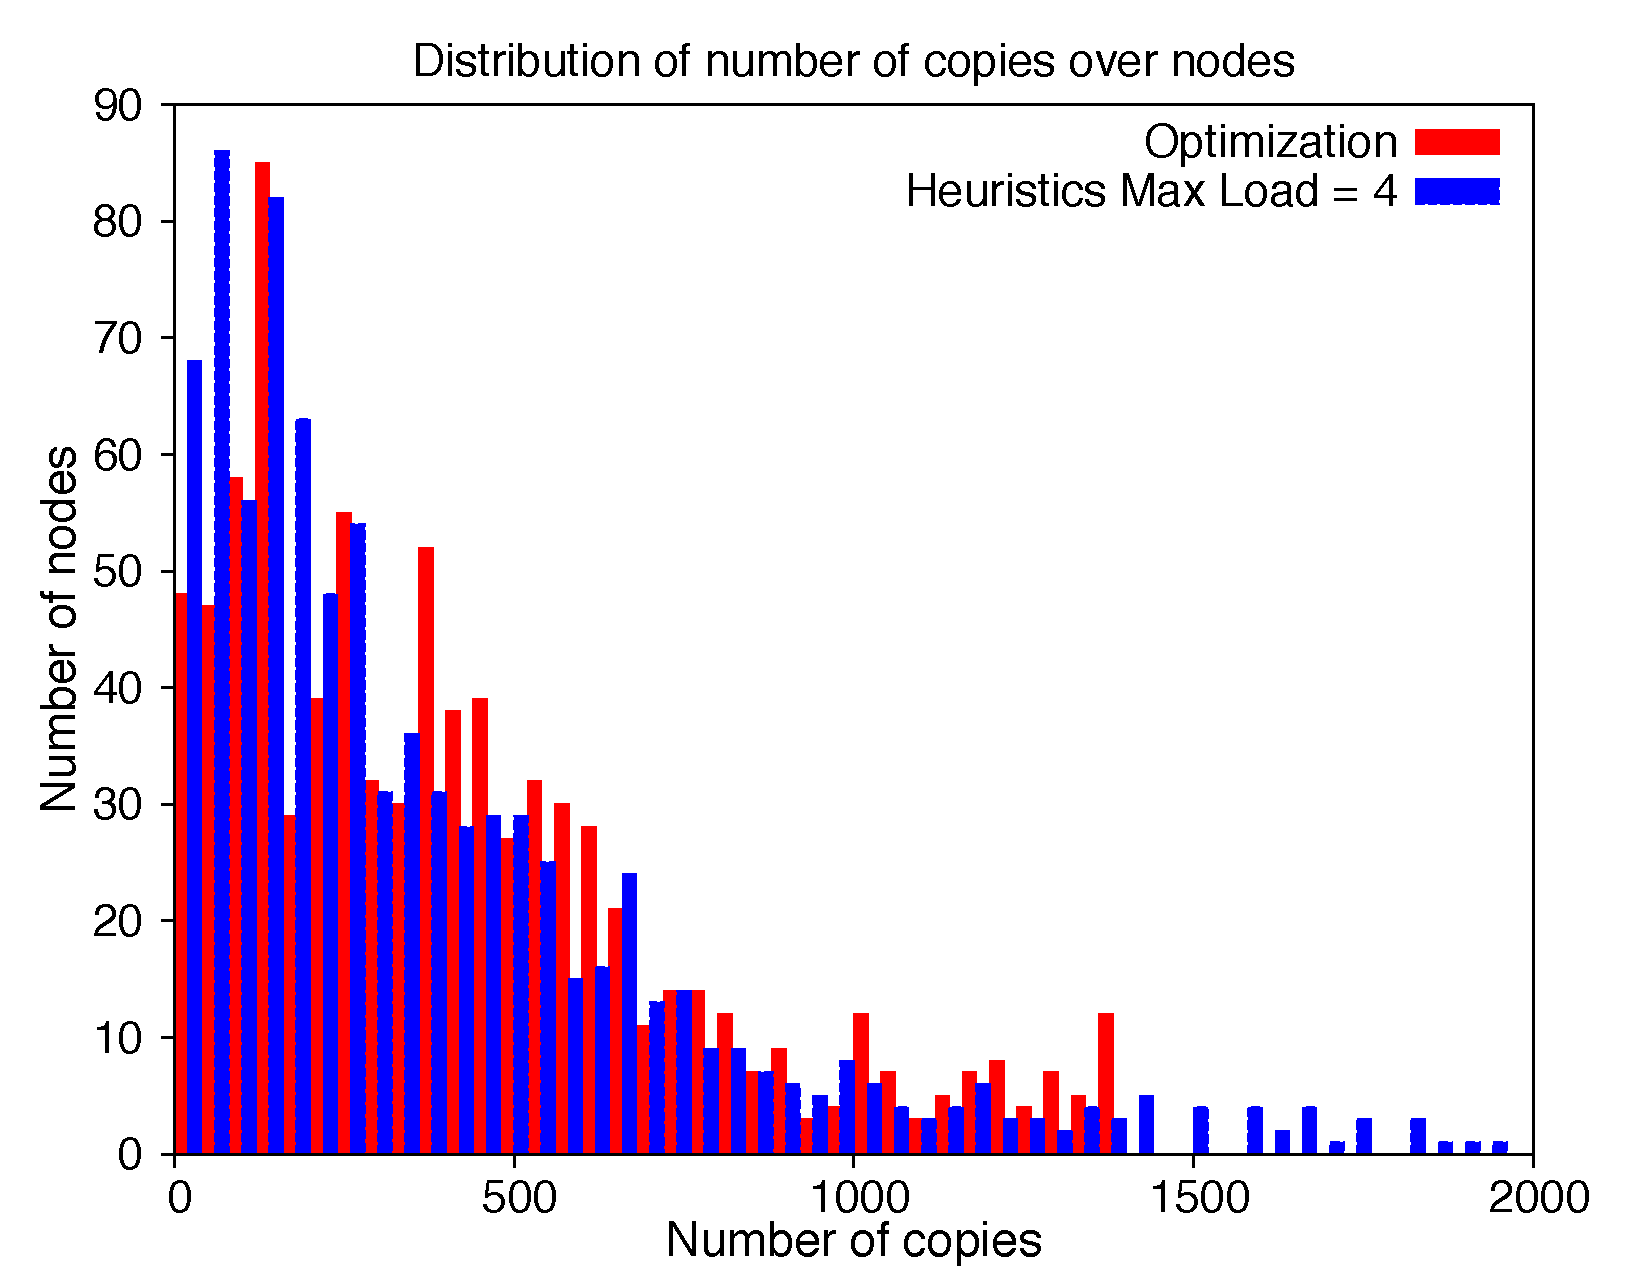
\includegraphics[width=\textwidth]{report_figures/constantr/3_1024/copy_histo.pdf}
                \caption{Distribution of number of copies over nodes}
                \label{fig:3_1024_copy}
        \end{subfigure}
        ~ %add desired spacing between images, e. g. ~, \quad, \qquad, \hfill etc.
          %(or a blank line to force the subfigure onto a new line)
        \begin{subfigure}[b]{0.49\textwidth}
                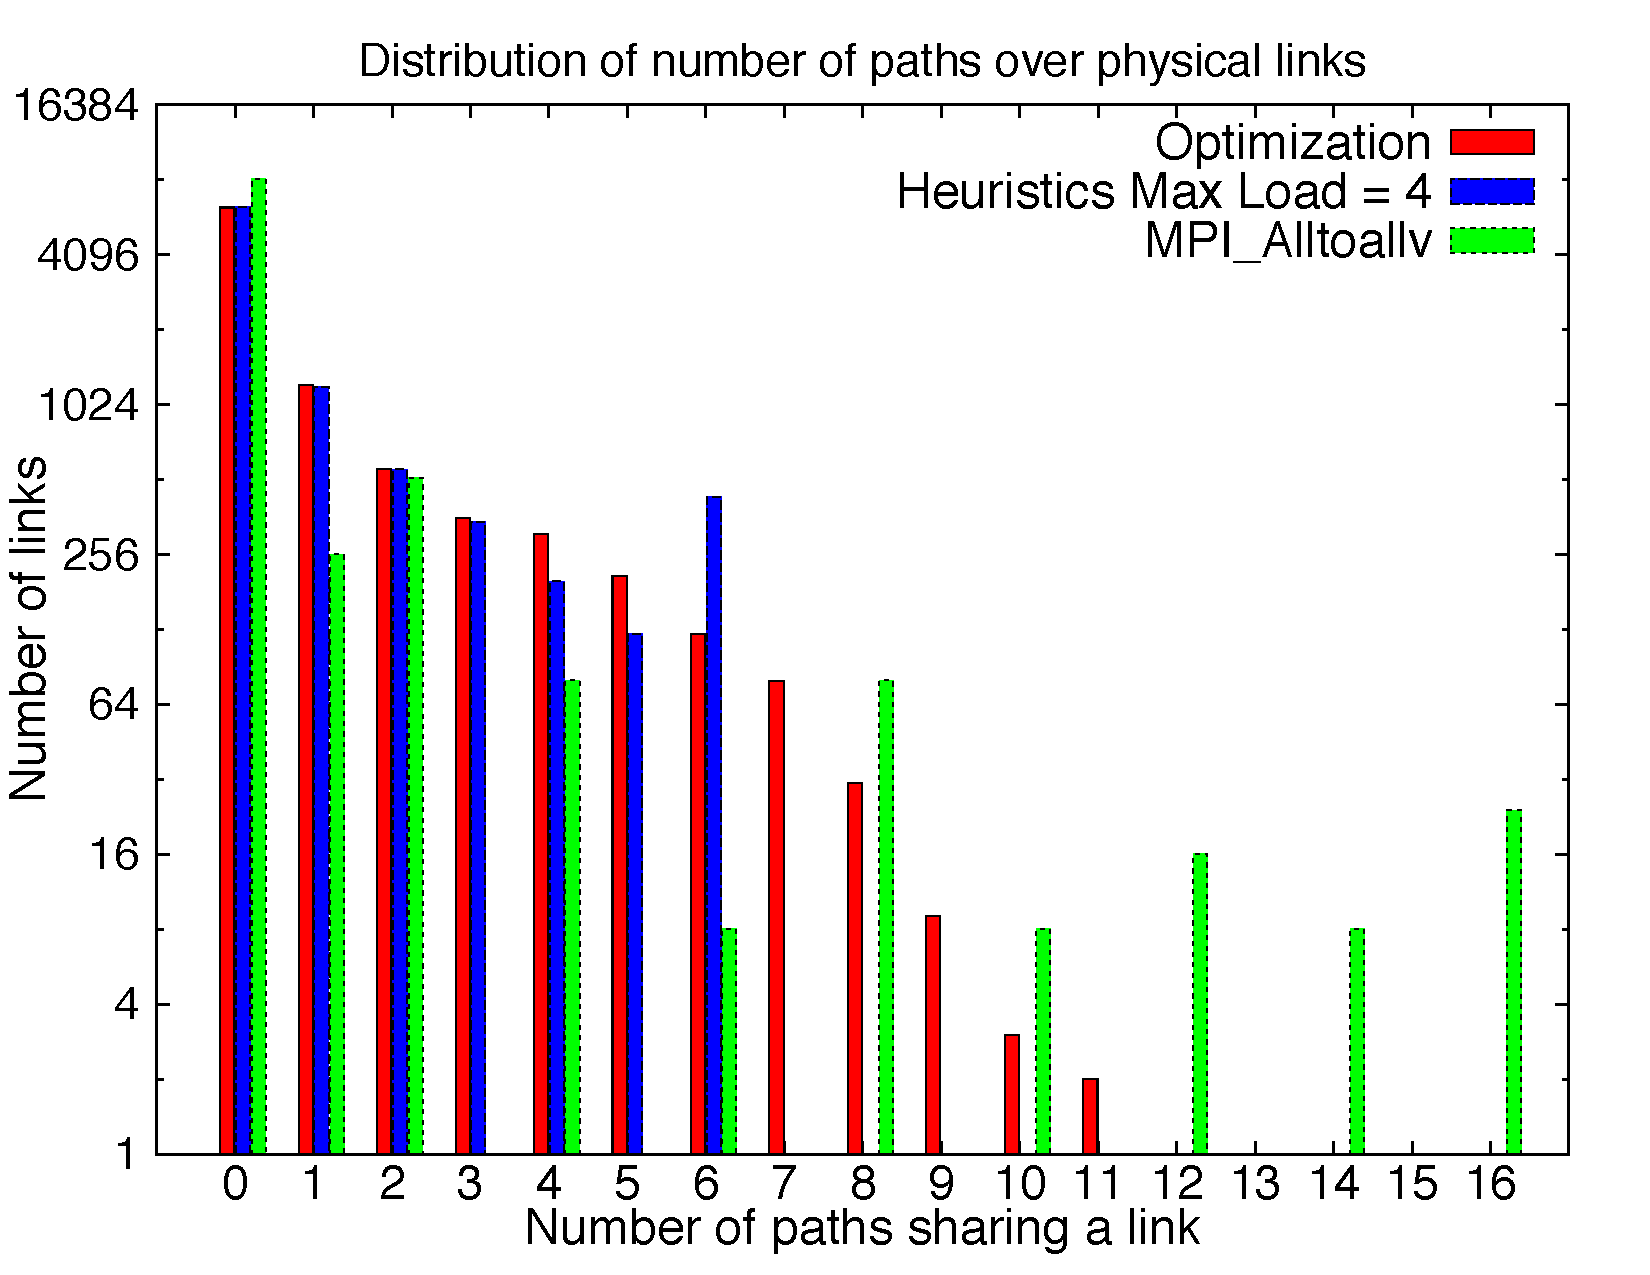
\includegraphics[width=\textwidth]{report_figures/constantr/3_1024/loadpath_histo.pdf}
                \caption{Distribution of number of paths over physicallinks}
                \label{fig:3_1024_loadpath}
        \end{subfigure}
        ~ %add desired spacing between images, e. g. ~, \quad, \qquad, \hfill etc.
          %(or a blank line to force the subfigure onto a new line)
        \begin{subfigure}[b]{0.49\textwidth}
                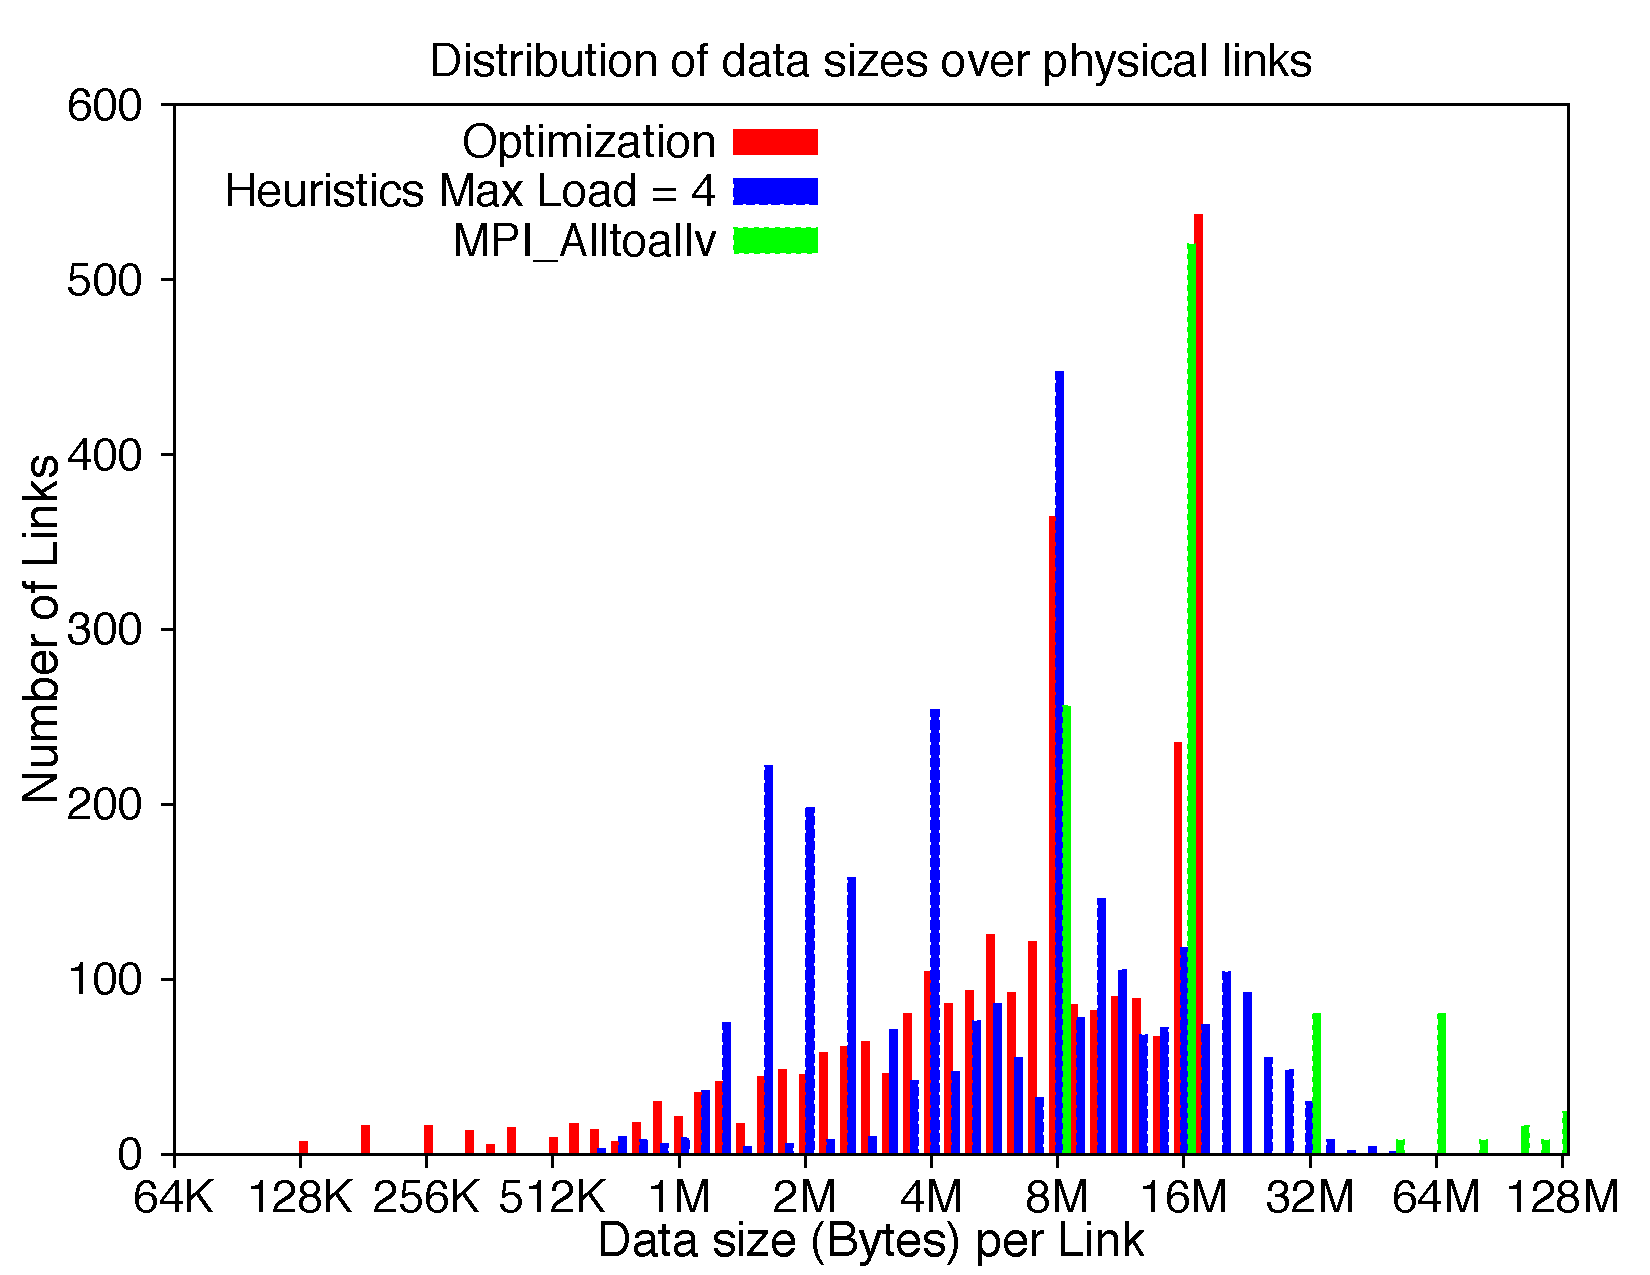
\includegraphics[width=\textwidth]{report_figures/constantr/3_1024/loaddata_histo.pdf}
                \caption{Distribution of total data size over physical links}
                \label{fig:3_1024_loaddata}
        \end{subfigure}
        ~ %add desired spacing between images, e. g. ~, \quad, \qquad, \hfill etc.
          %(or a blank line to force the subfigure onto a new line)
        \begin{subfigure}[b]{0.49\textwidth}
                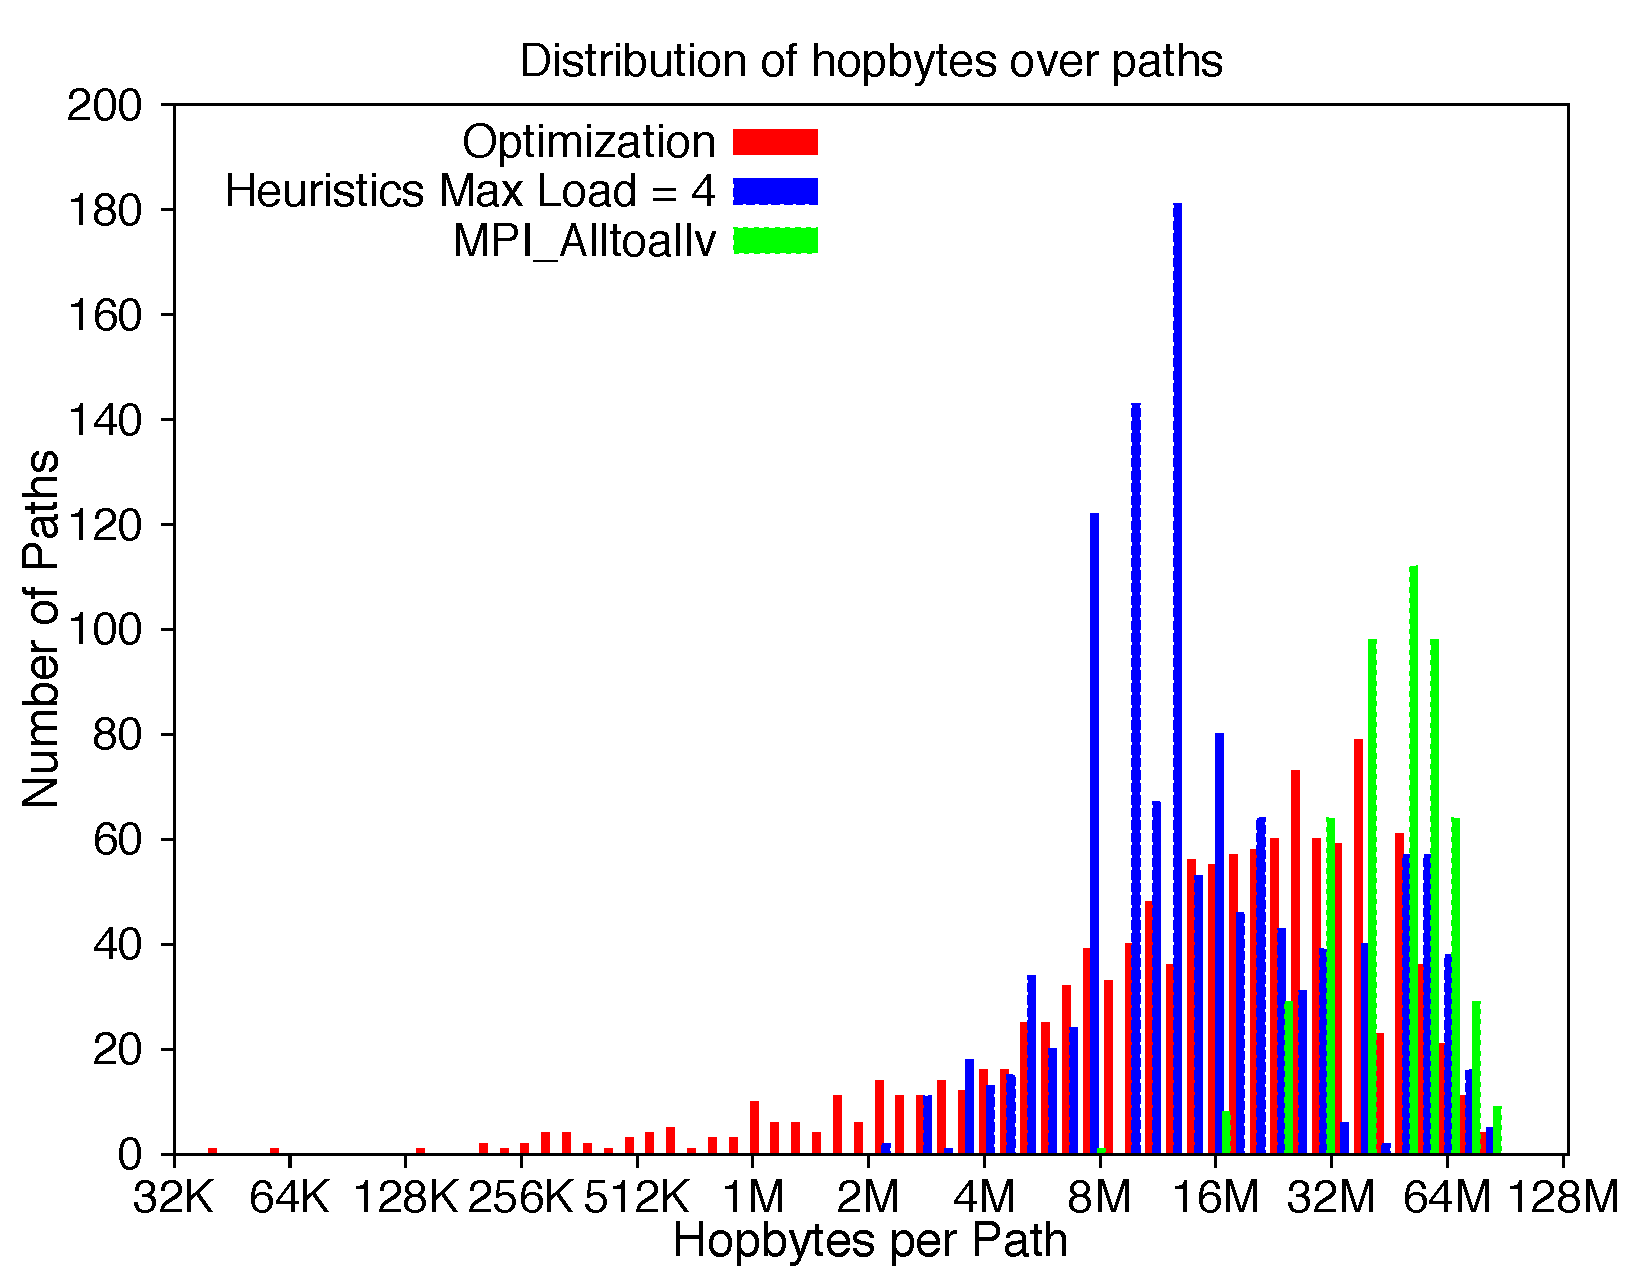
\includegraphics[width=\textwidth]{report_figures/constantr/3_1024/hopbyte_histo.pdf}
                \caption{Distribution of hopbytes over paths}
                \label{fig:3_1024_hopbyte}
        \end{subfigure}
        ~ %add desired spacing between images, e. g. ~, \quad, \qquad, \hfill etc.
          %(or a blank line to force the subfigure onto a new line)
        \begin{subfigure}[b]{0.49\textwidth}
                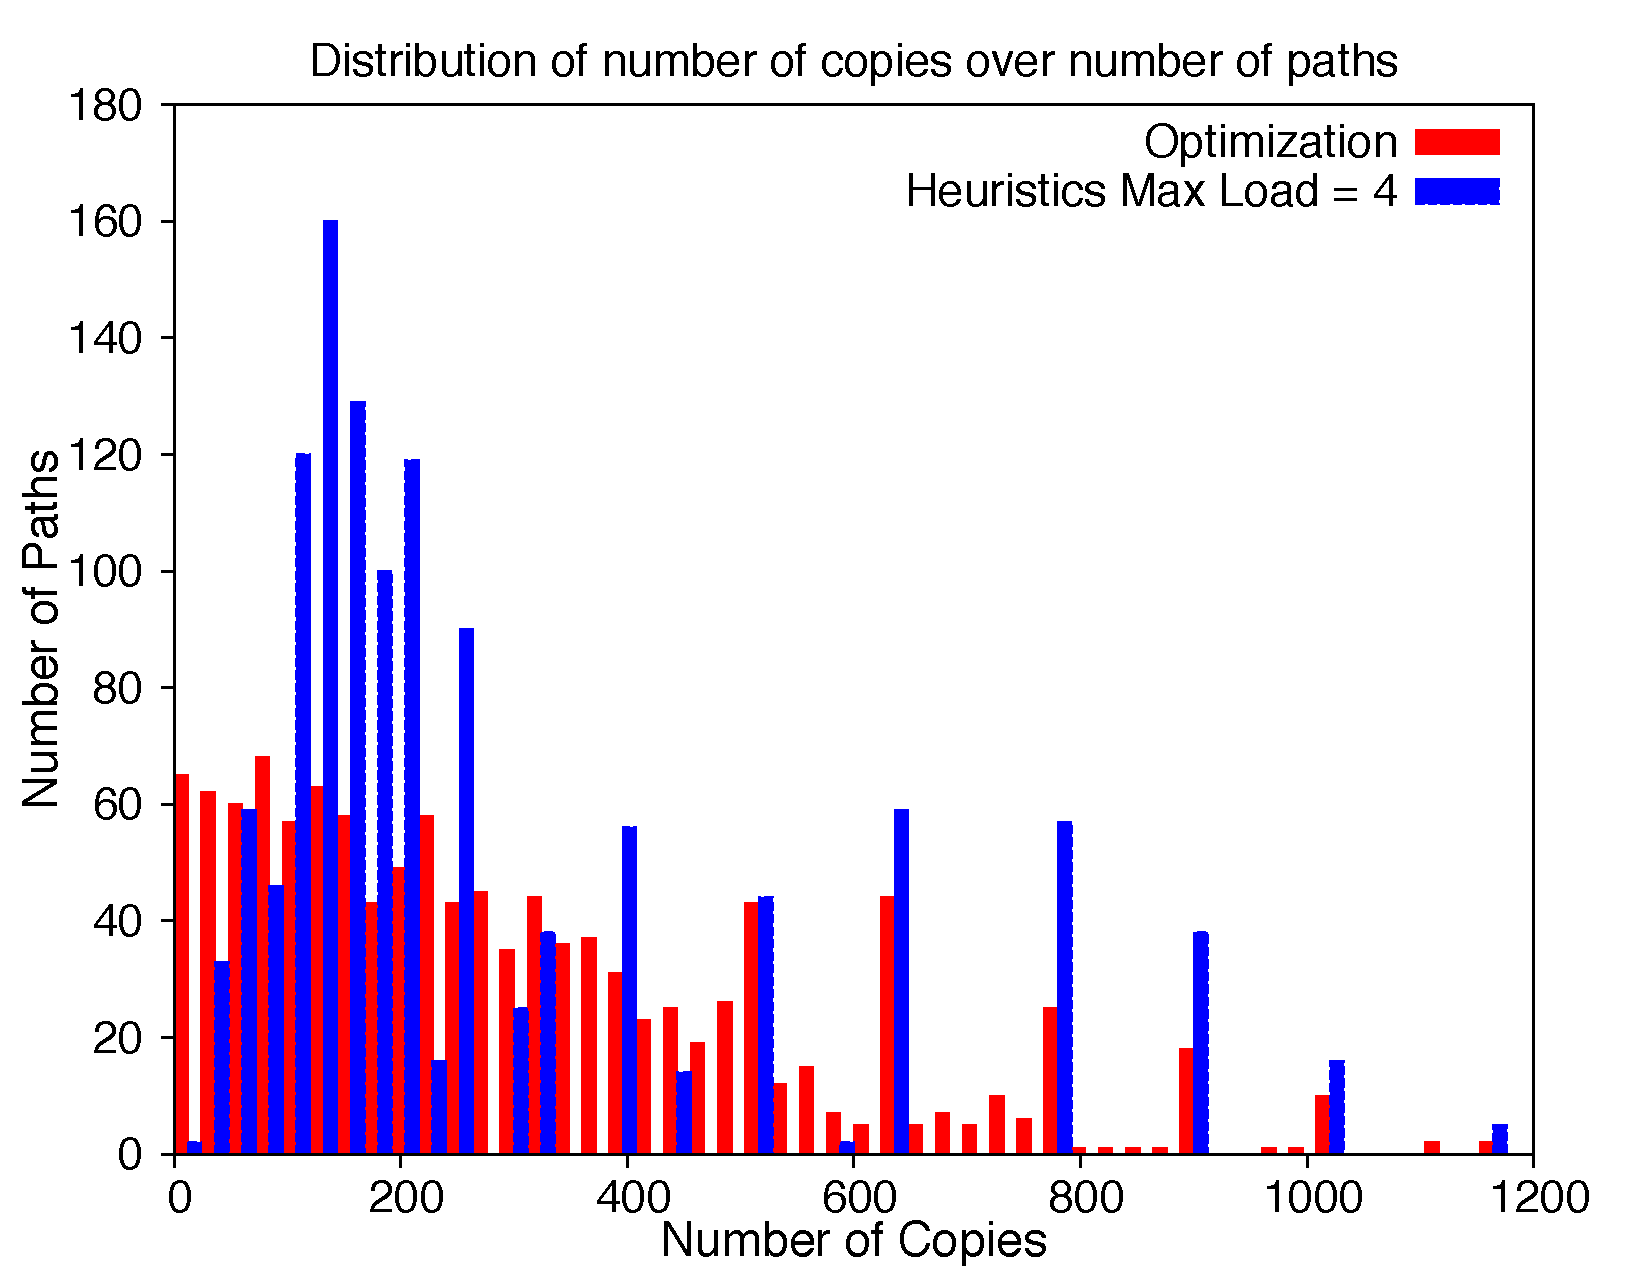
\includegraphics[width=\textwidth]{report_figures/constantr/3_1024/hopcopy_histo.pdf}
                \caption{Distribution of number of copies over paths}
                \label{fig:3_1024_hopcopy}
        \end{subfigure}
        \caption{Historgram of hops, copies, load in terms of number of paths and data size}
        \label{fig:3_1024_histo}
\end{figure}



\newpage

\subsubsection{Number of nodes 2048}

\input{tables/tables_3_2048.dat}

\newpage

\subsubsection{Number of nodes 4096}

\input{tables/tables_3_4096.dat}

\newpage

\subsection{Overlap set - Test Id = 27}

Among N nodes, N/2 source nodes send data to N/16 destination nodes. The destination nodes are among the source nodes. There are N/2 pairs of communication, 8 MB of data per pair. There is 1 MPI/PAMI rank per node. Experiments are done for N=512, 1024, 2048, 4096 and 8192 nodes.

\begin{figure}[h]
\vspace{-0.1in}
\centering
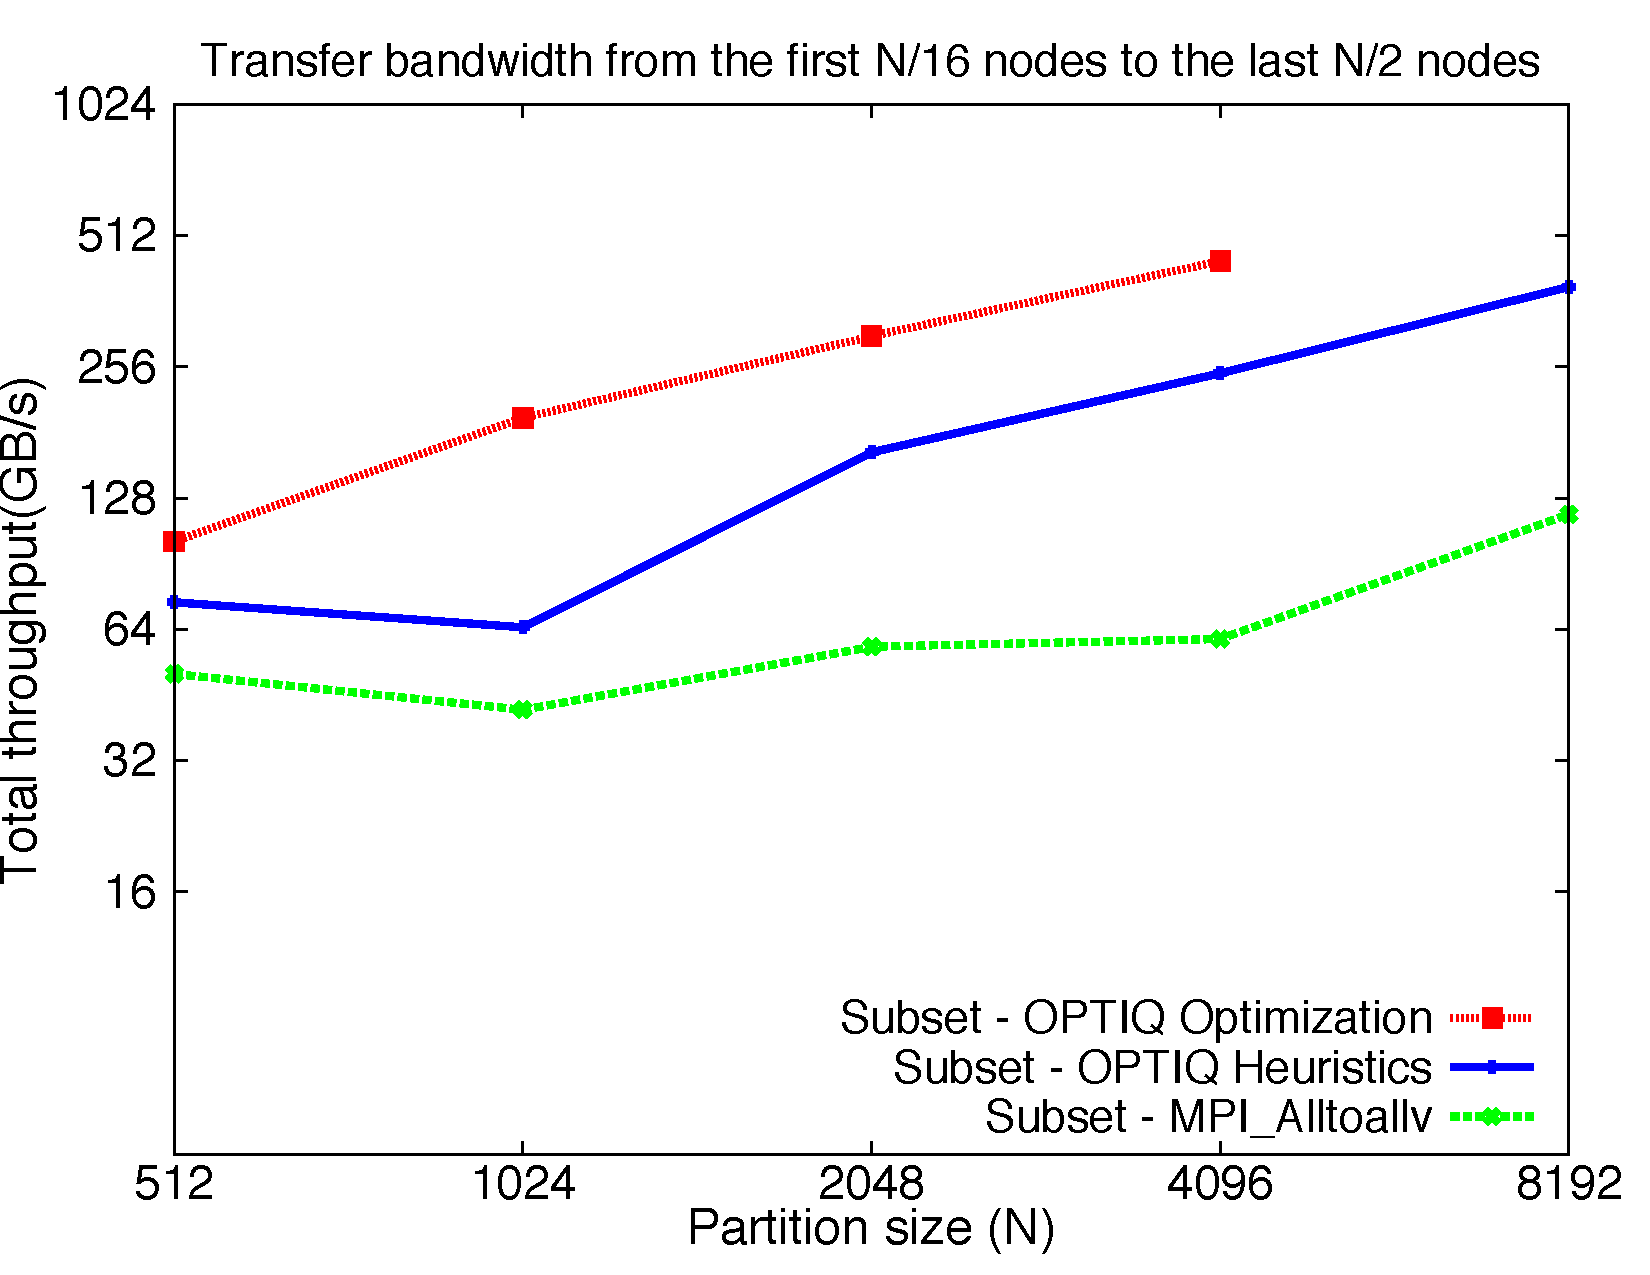
\includegraphics[scale=0.40]{report_figures/constantr_27.pdf}
\vspace{-0.1in}
\caption{Overlap performance}
\vspace{-0.1in}
\label{fig:patterns}
\end{figure}

\newpage

\subsubsection{Number of nodes 512}

\input{tables/tables_27_512.dat}

\newpage

\subsubsection{Number of nodes 1024}

\input{tables/tables_27_1024.dat}

\newpage

\subsubsection{Number of nodes 2048}

\input{tables/tables_27_2048.dat}

\newpage

\subsubsection{Number of nodes 4096}

\input{tables/tables_27_4096.dat}

\newpage

\subsection{Subset tests - Test Id = 87}

Among N nodes, N/2 source nodes send data to N/16 destination nodes. The destination nodes are among the source nodes. There are N/2 pairs of communication, 8 MB of data per pair. There is 1 MPI/PAMI rank per node. Experiments are done for N=512, 1024, 2048, 4096 and 8192 nodes.

\begin{figure}[h]
\vspace{-0.1in}
\centering
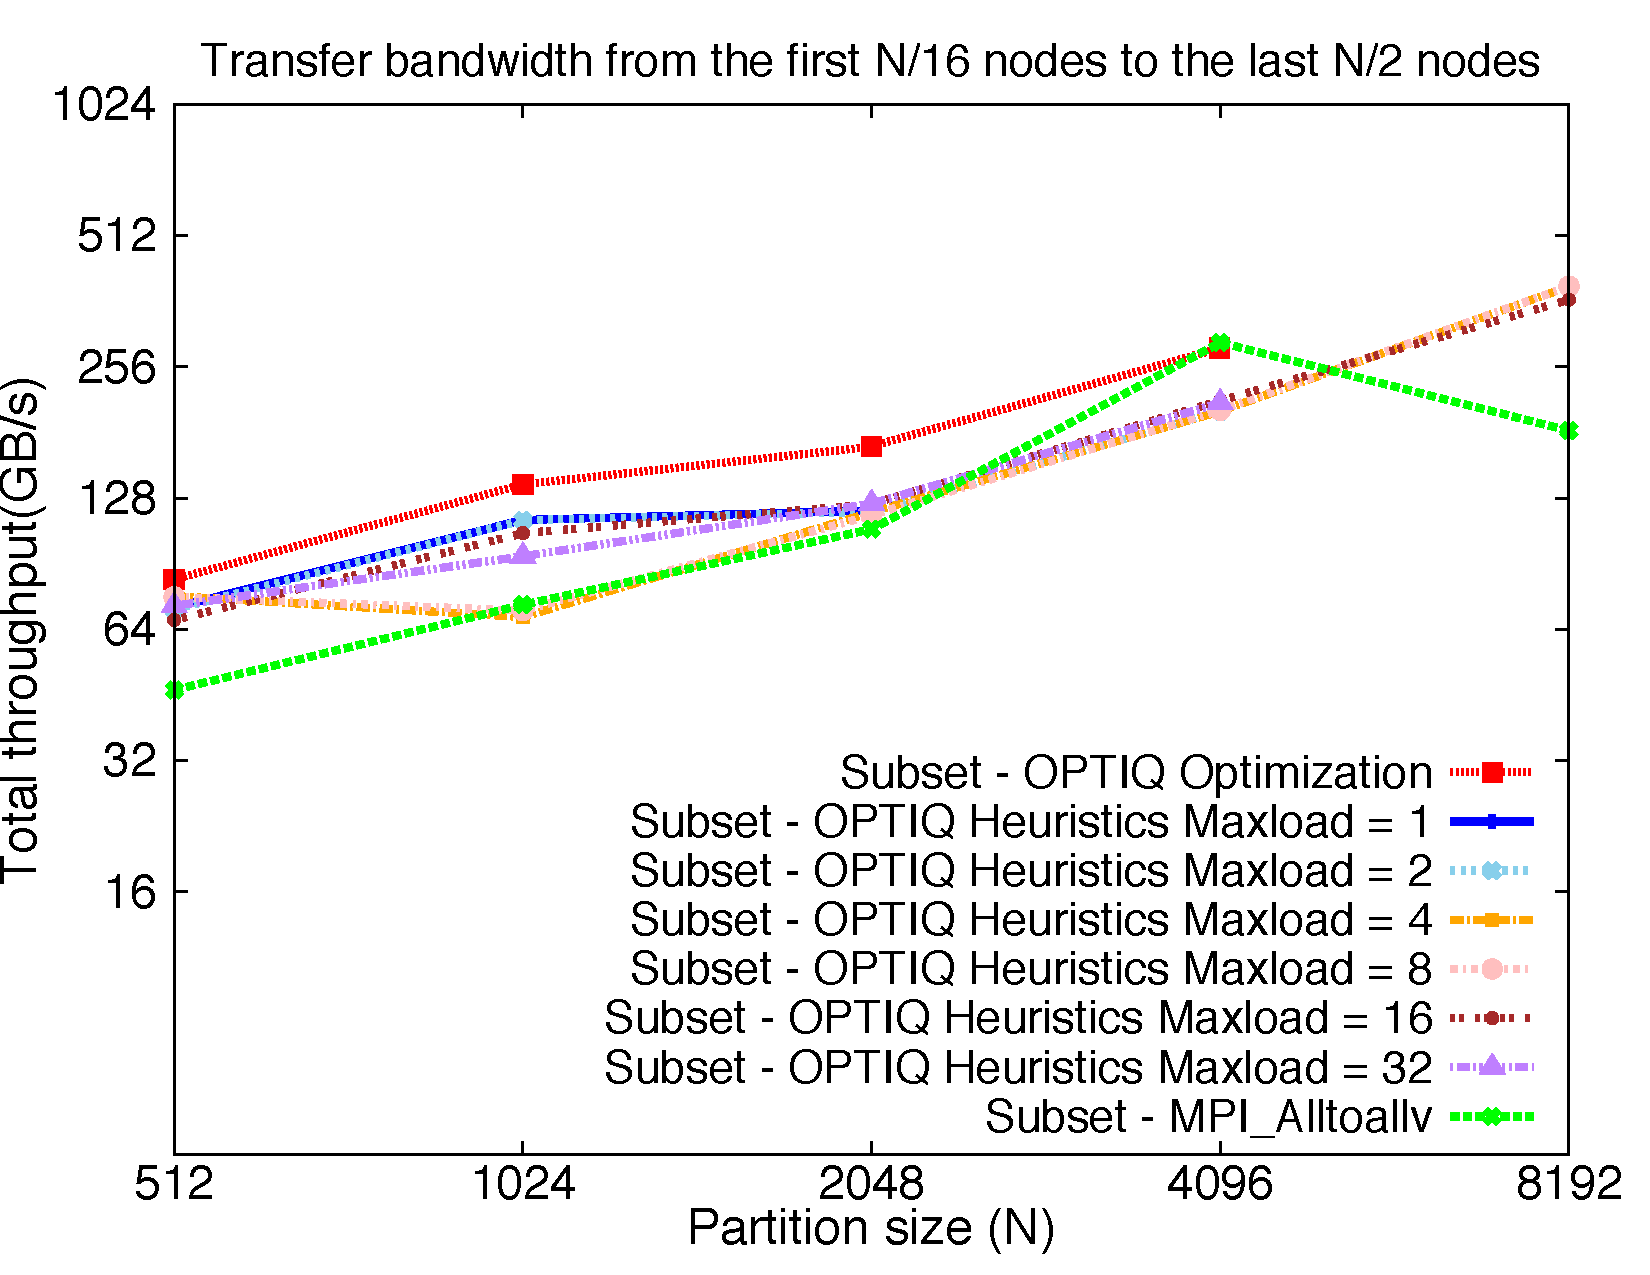
\includegraphics[scale=0.40]{report_figures/constantr_87.pdf}
\vspace{-0.1in}
\caption{Subset performance}
\vspace{-0.1in}
\label{fig:patterns}
\end{figure}

\subsubsection {Total number of nodes 512}

Source nodes are the first 256 nodes (nodes 0 to 255), destination nodes are 32 nodes in the middle of the source nodes (nodes 128 to 159). There are 256 pairs of communication, 8 MB of data per pair. As 32 destination nodes are contiguous, per each node out of 10 links, 6 links along C, D, E dimensions are used for internal interconnection (connect nodes among 32 nodes). The 4 remaining links along A and B dimensions are used to interconnect with nodes outside of the destination set. Thus, the maximum achievable throughput is 32 (nodes) x 4 (links/node) x 1.7 (GB/s/link) = 217.6 (GB/s). The experiments were carried with Optimization, Heuristics and MPI\_Alltoallv. For Optimization, 50 paths were fed into optimization model per job (12800 paths total). For Heuristics, we selected paths with max load = 4. Table \ref{table:512_perf} shows the performance and path-related information. Table \ref{table:512_hopcopy} and \ref{table:512_load} show number of hops, number of copies and loads of the experiments. Figure \ref{fig:512_histo} shows the histogram (distribution) of number of hops, number of copies, number of paths sharing physical links and total amount of data traveling through a physical link.

Table \ref{table:512_perf} shows that Optimization throughput (83 GB/s) is a slightly higher than Heuristics (76 GB/s), and both are significantly higher than MPI\_Alltoallv (47 GB/s). It also shows that Optimization used 621 paths, Heuristics used 524 paths and MPI used 256 paths. Per job, Optimization has highest max, median and average number of paths. Because Optmization has highest number of paths, it also has highest total number of hops. However per path, the max, min, average and median number of of hops are very similar among Optimization, Heuristics and MPI\_Alltoallv, shown in Table \ref{table:512_hopcopy} and Figure \ref{fig:512_hop}. 

When data travels along the paths, it is split into small chunks, copied and injected again to the interconnect network at intermediate nodes. The number of copies can cause some delays thus, degrade throughput. In comparison to Heuristics, Optimization has higher total of number of copies but lower max, min, average and median number of copies per node, shown in Table \ref{table:512_load} and Figure \ref{fig:512_copy}. This is because it used more paths and nodes and thus spreaded the copies over more nodes. This can lead to better performance for Optmization.

Regarding loads over physical links, we consider two types of load on physical links: the number of paths that use a physical link and the actual amount of data travels through a physical link, shown in Table \ref{table:512_load}. While the number of paths load only reveals how many paths use a particular link, it does not reveal how much data actual travels through that particular link, which is more important in investigating performance. As the Table \ref{table:512_load} and Figure \ref{fig:512_loadpath} \& \ref{fig:512_loaddata}  show, Optmization has highest number paths per physical link, but it actually has lowest actual amount of data load. This is because Optimization split the data among paths and thus led to more balanced data load.

In conclusion, Optimization throughput (83 GB/s) is a slightly higher than Heuristics (76 GB/s), and both are significantly higher than MPI\_Alltoallv (47 GB/s). The reasons include:
\begin{itemize}
\item Optimization and Heuristics used more paths than MPI\_Alltoallv. MPI\_Alltoallv has only 256 paths, Heuristics has 524 and Optimization has 621 - Table \ref{table:512_perf}.
\item Optimization and Heursitcs has lower maximum load than MPI\_Alltoallv in terms of total amount of data over physical links. The maximum number of paths sharing in case of Optimization is 9 which is higher than both Heuristics (at most 4 paths per link) and MPI\_Alltoallv (at most 6 paths per link). However, because we split data on different paths in case of Optimization, we ended up with least maximum total amount of data per link. That contributes to better performance for Optimization - Table \ref{table:512_load} and Figure \ref{fig:512_loadpath} \& \ref{fig:512_loaddata}.
\item They all have approximately number of hops (max, min, avg and med) - Table \ref{table:512_hopcopy} and Figure \ref{fig:512_hop}.
\item Optimization has lower maximum number of copies and the copies ditribution is better than Heuristics - Table \ref{table:512_hopcopy} and Figure \ref{fig:512_copy}.
\end{itemize}

\newpage

\input{tables/tables_87_512.dat}

\begin{figure}[!htbp]
        \centering
        \begin{subfigure}[b]{0.49\textwidth}
                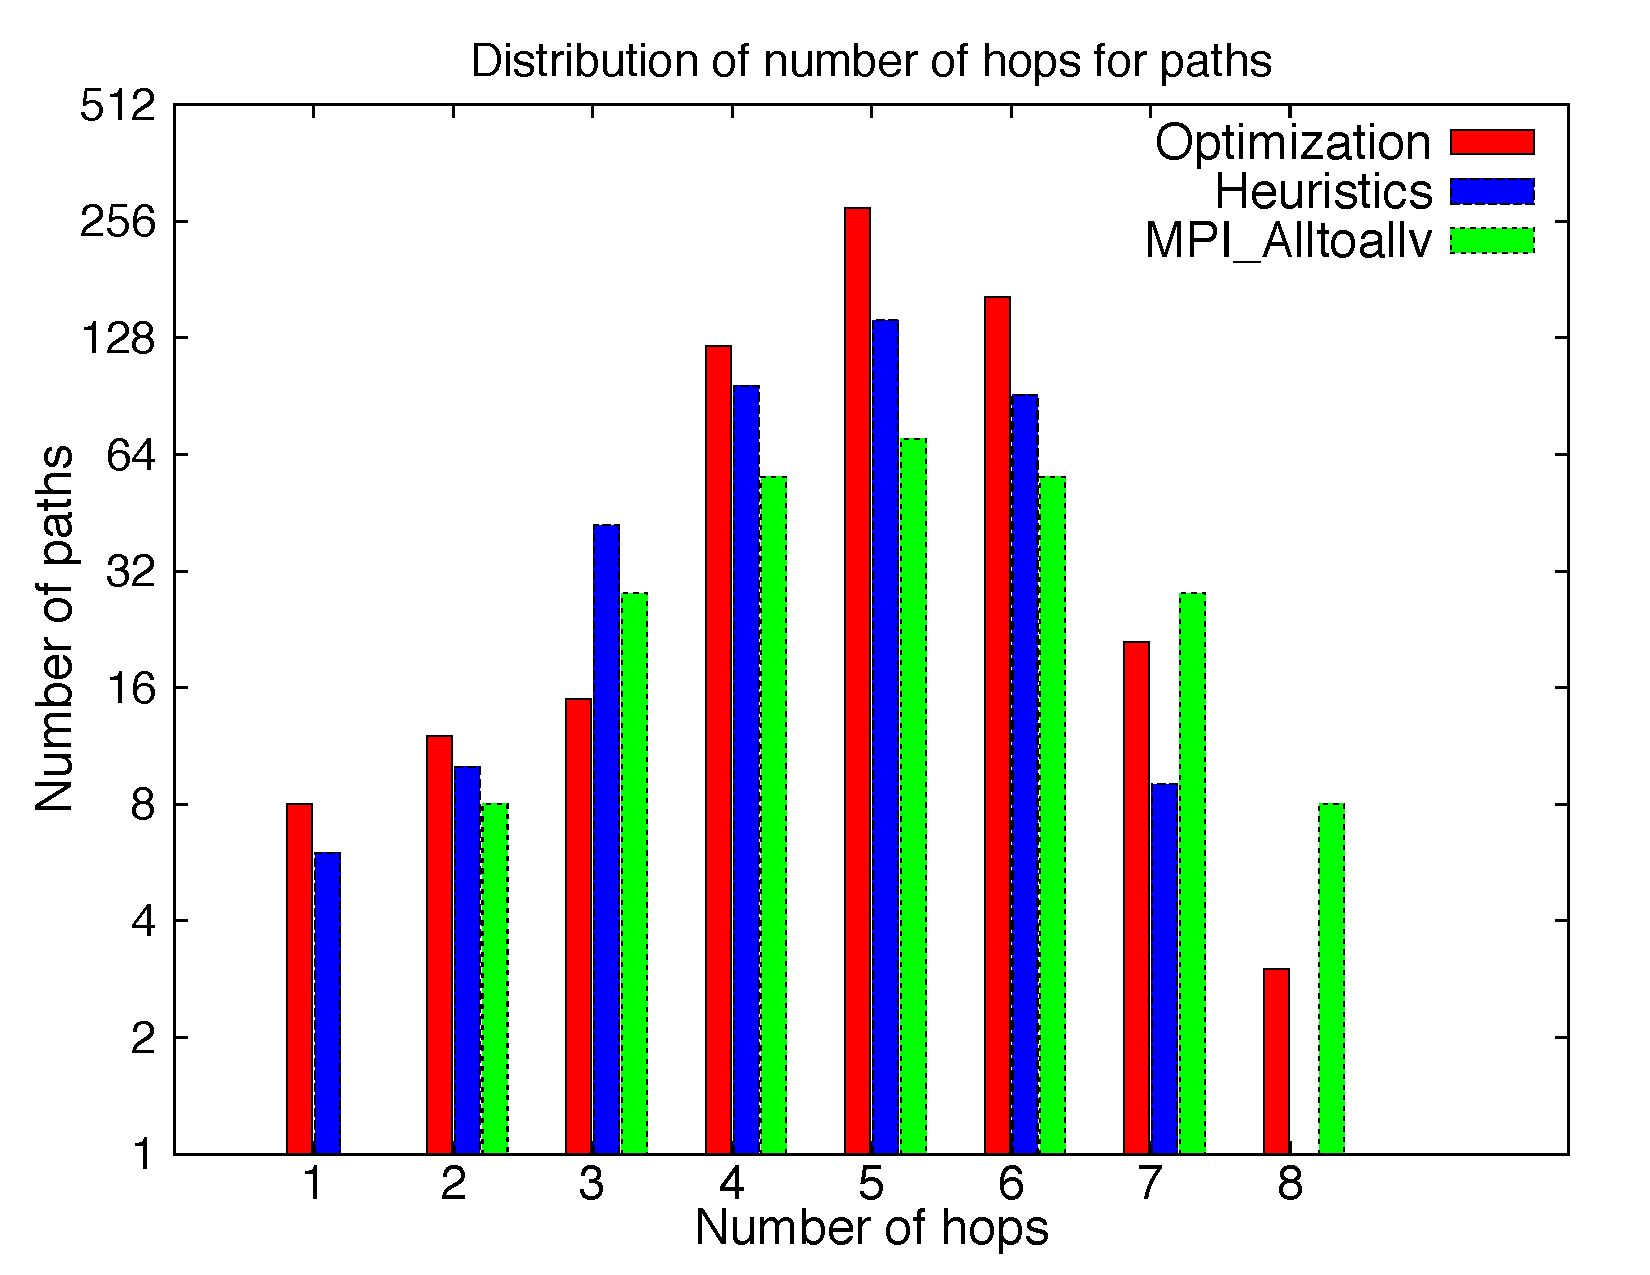
\includegraphics[width=\textwidth]{report_figures/hop_histo.pdf}
                \caption{Distribution of number of hops over paths}
                \label{fig:512_hop}
        \end{subfigure}%
        ~ %add desired spacing between images, e. g. ~, \quad, \qquad, \hfill etc.
          %(or a blank line to force the subfigure onto a new line)
        \begin{subfigure}[b]{0.49\textwidth}
                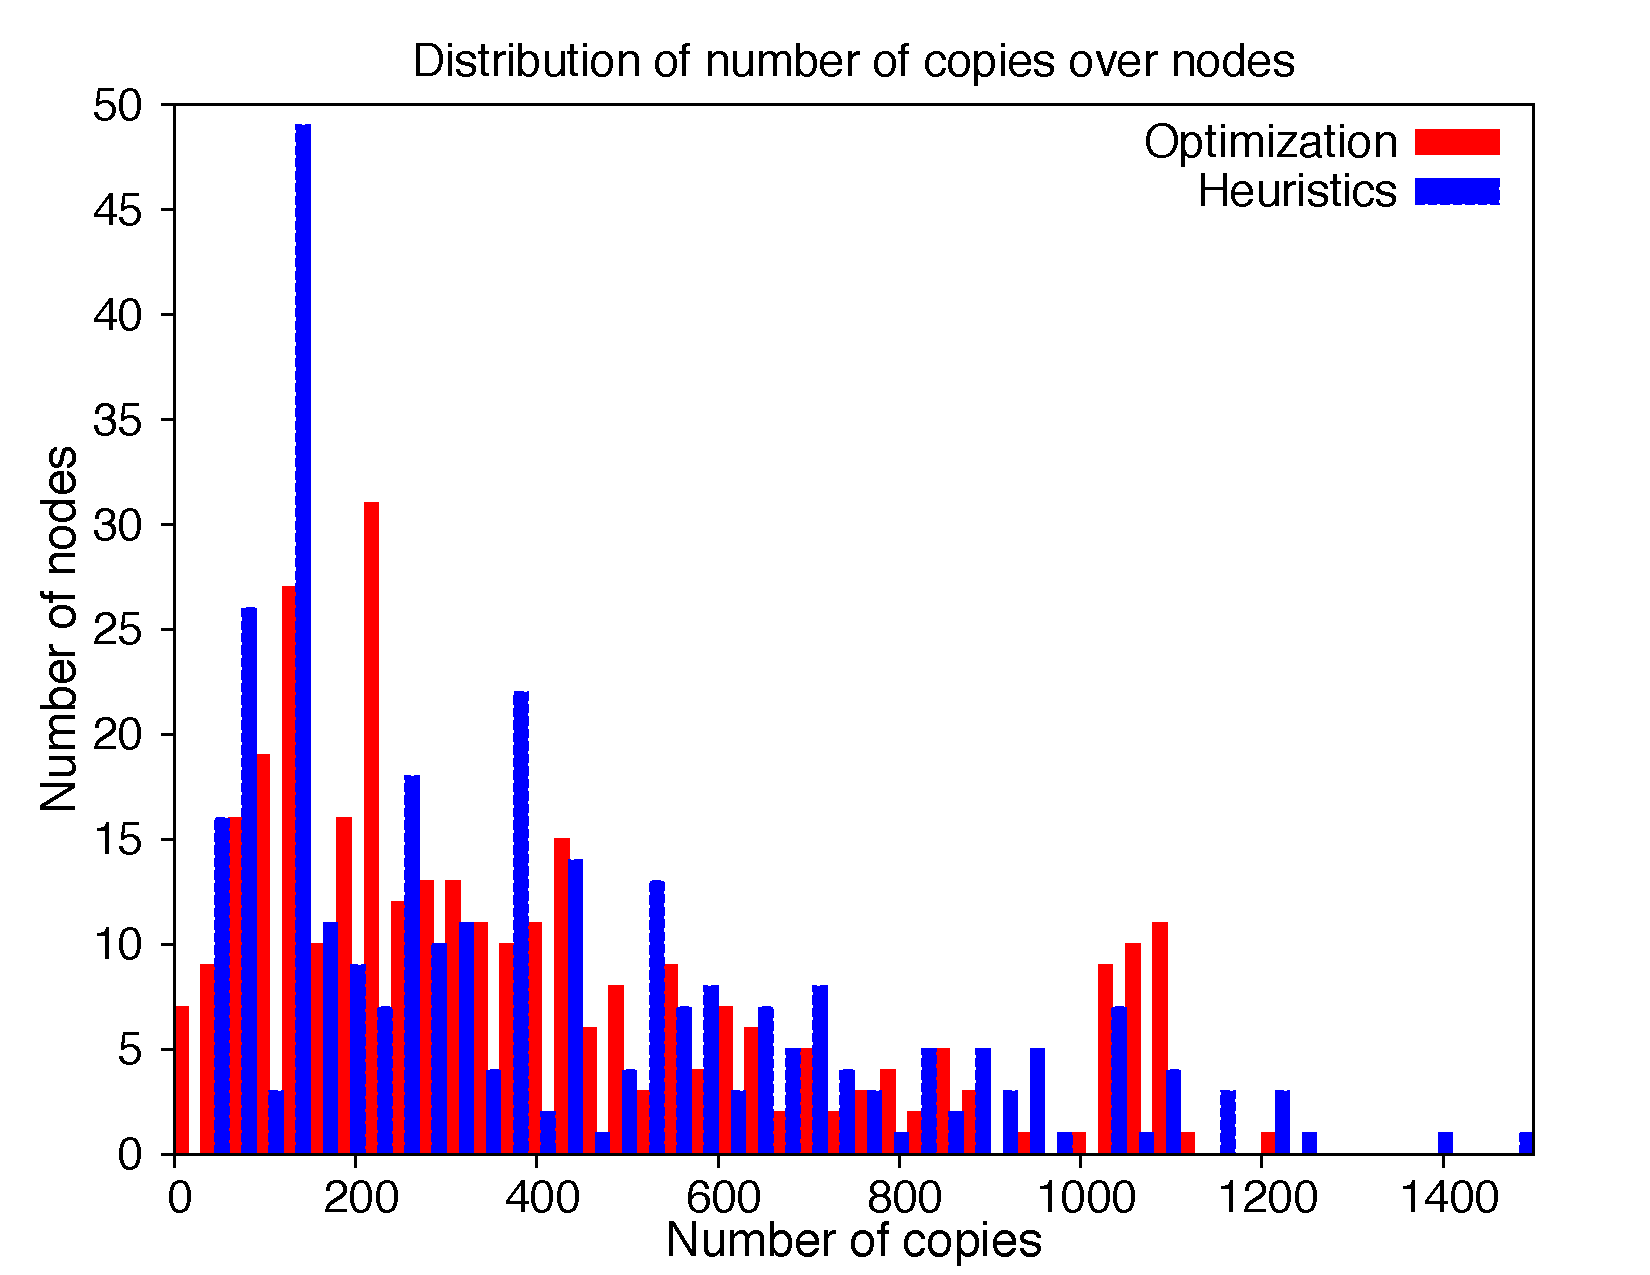
\includegraphics[width=\textwidth]{report_figures/copy_histo.pdf}
                \caption{Distribution of number of copies over nodes}
                \label{fig:512_copy}
        \end{subfigure}
        ~ %add desired spacing between images, e. g. ~, \quad, \qquad, \hfill etc.
          %(or a blank line to force the subfigure onto a new line)
        \begin{subfigure}[b]{0.49\textwidth}
                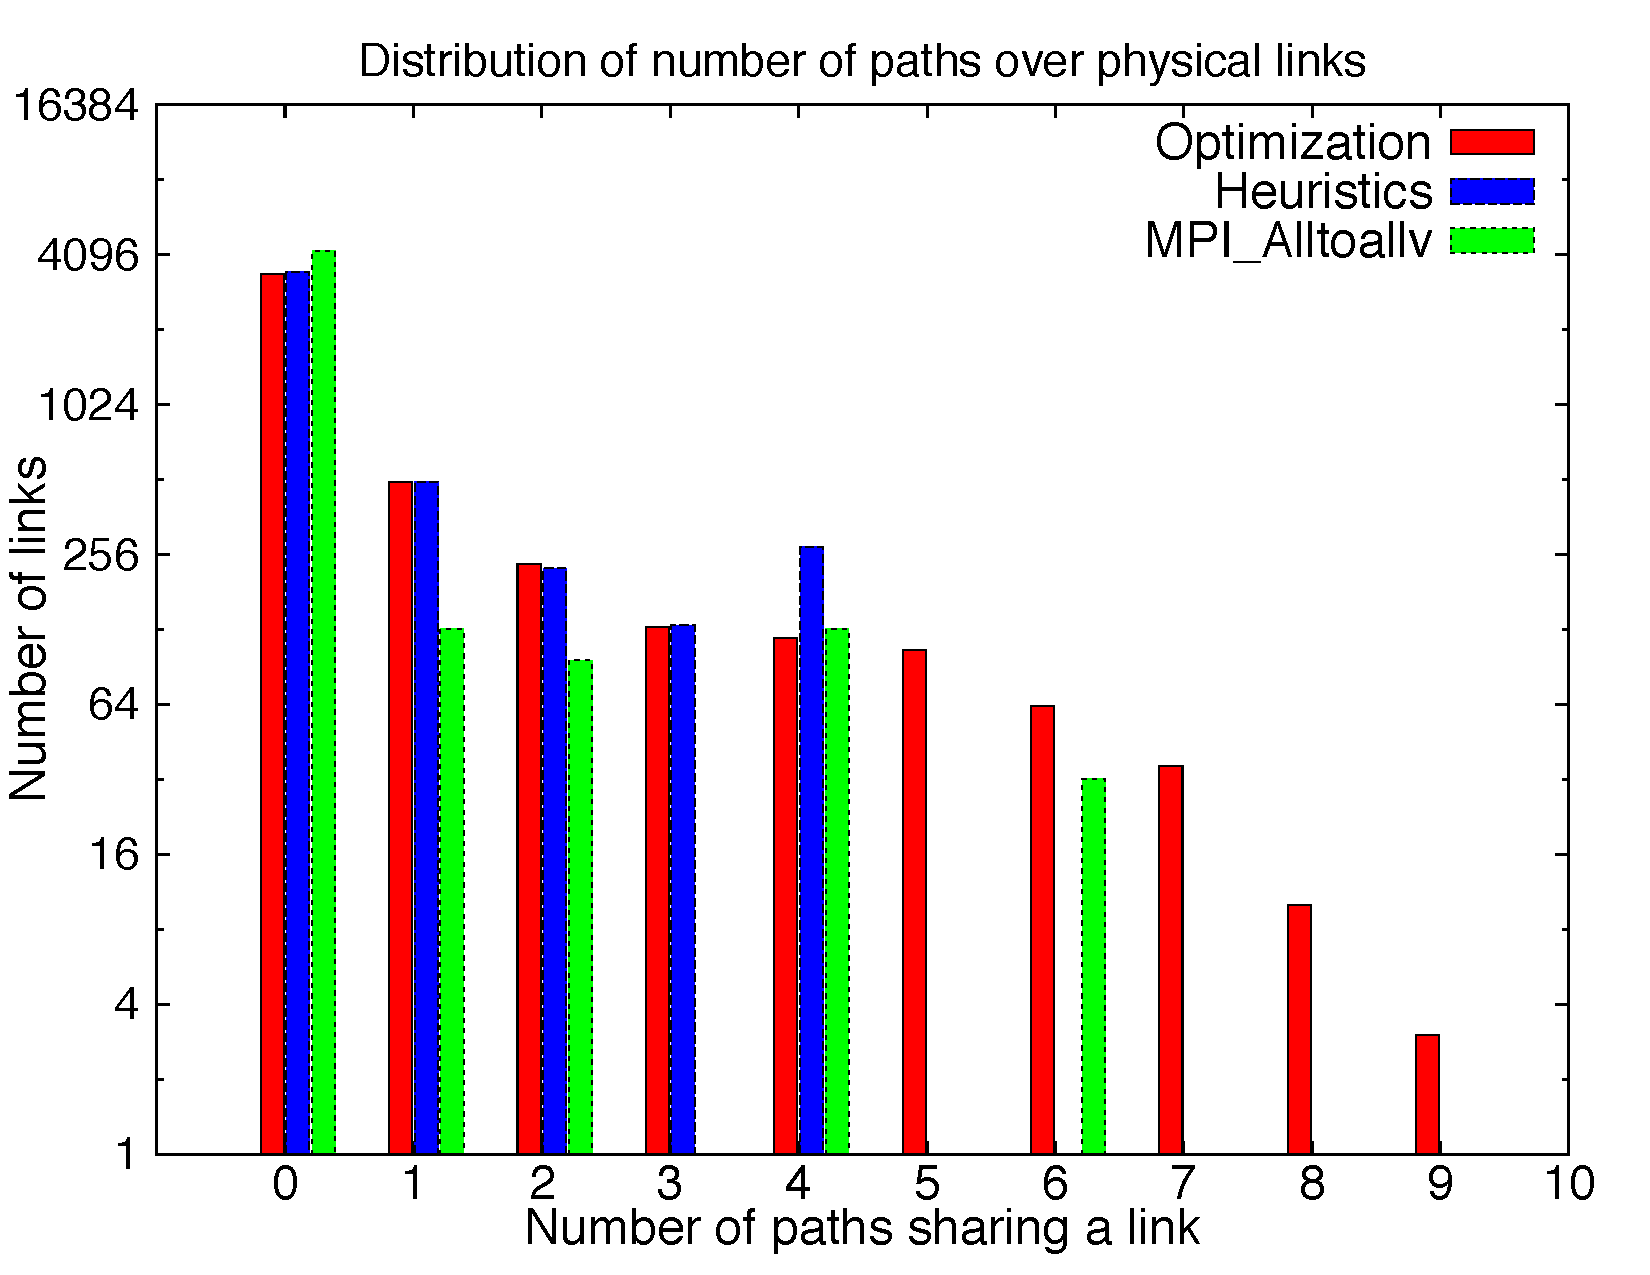
\includegraphics[width=\textwidth]{report_figures/loadpath_histo.pdf}
                \caption{Distribution of number of paths over physicallinks}
                \label{fig:512_loadpath}
        \end{subfigure}
	~ %add desired spacing between images, e. g. ~, \quad, \qquad, \hfill etc.
          %(or a blank line to force the subfigure onto a new line)
	\begin{subfigure}[b]{0.49\textwidth}
                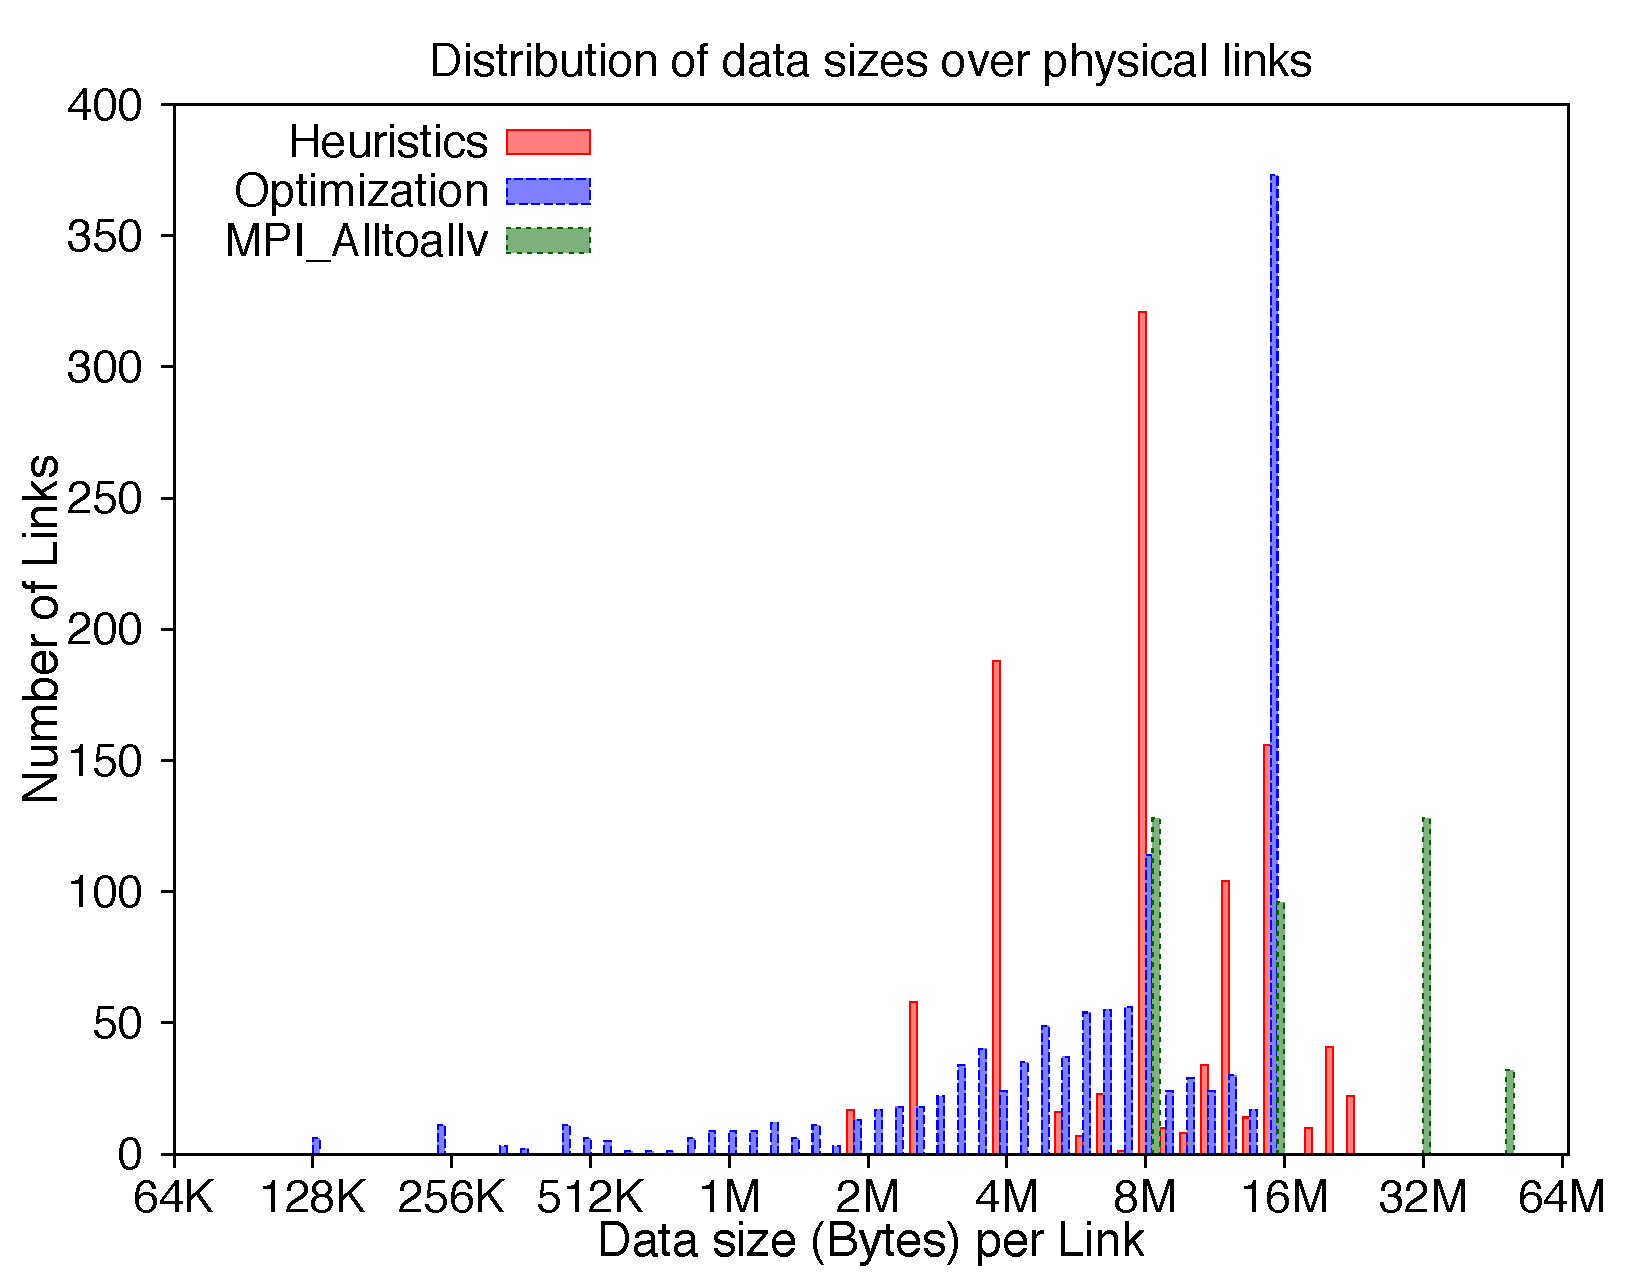
\includegraphics[width=\textwidth]{report_figures/loaddata_histo.pdf}
                \caption{Distribution of total data size over physical links}
                \label{fig:512_loaddata}
        \end{subfigure}
	~ %add desired spacing between images, e. g. ~, \quad, \qquad, \hfill etc.
          %(or a blank line to force the subfigure onto a new line)
        \begin{subfigure}[b]{0.49\textwidth}
                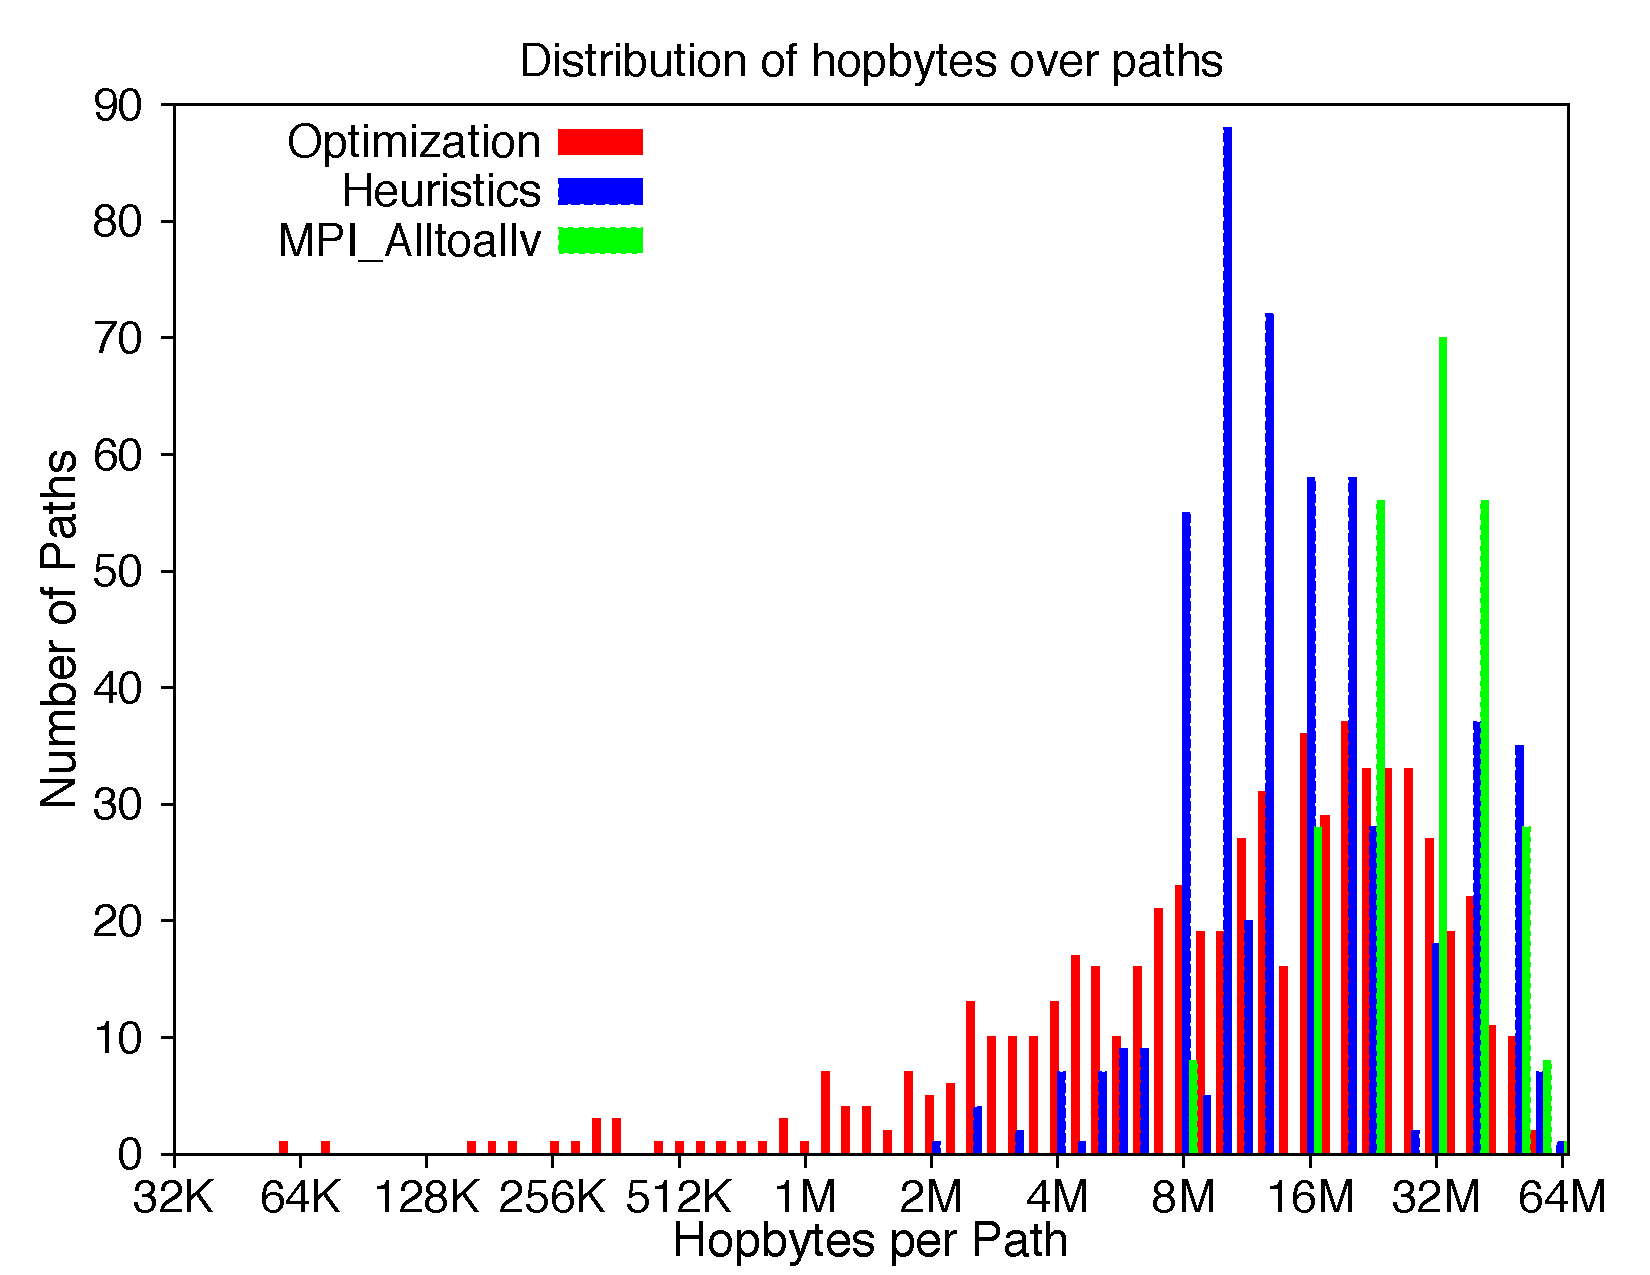
\includegraphics[width=\textwidth]{report_figures/hopbyte_histo.pdf}
                \caption{Distribution of hopbytes over paths}
                \label{fig:512_hopbyte}
        \end{subfigure}
	~ %add desired spacing between images, e. g. ~, \quad, \qquad, \hfill etc.
          %(or a blank line to force the subfigure onto a new line)
        \begin{subfigure}[b]{0.49\textwidth}
                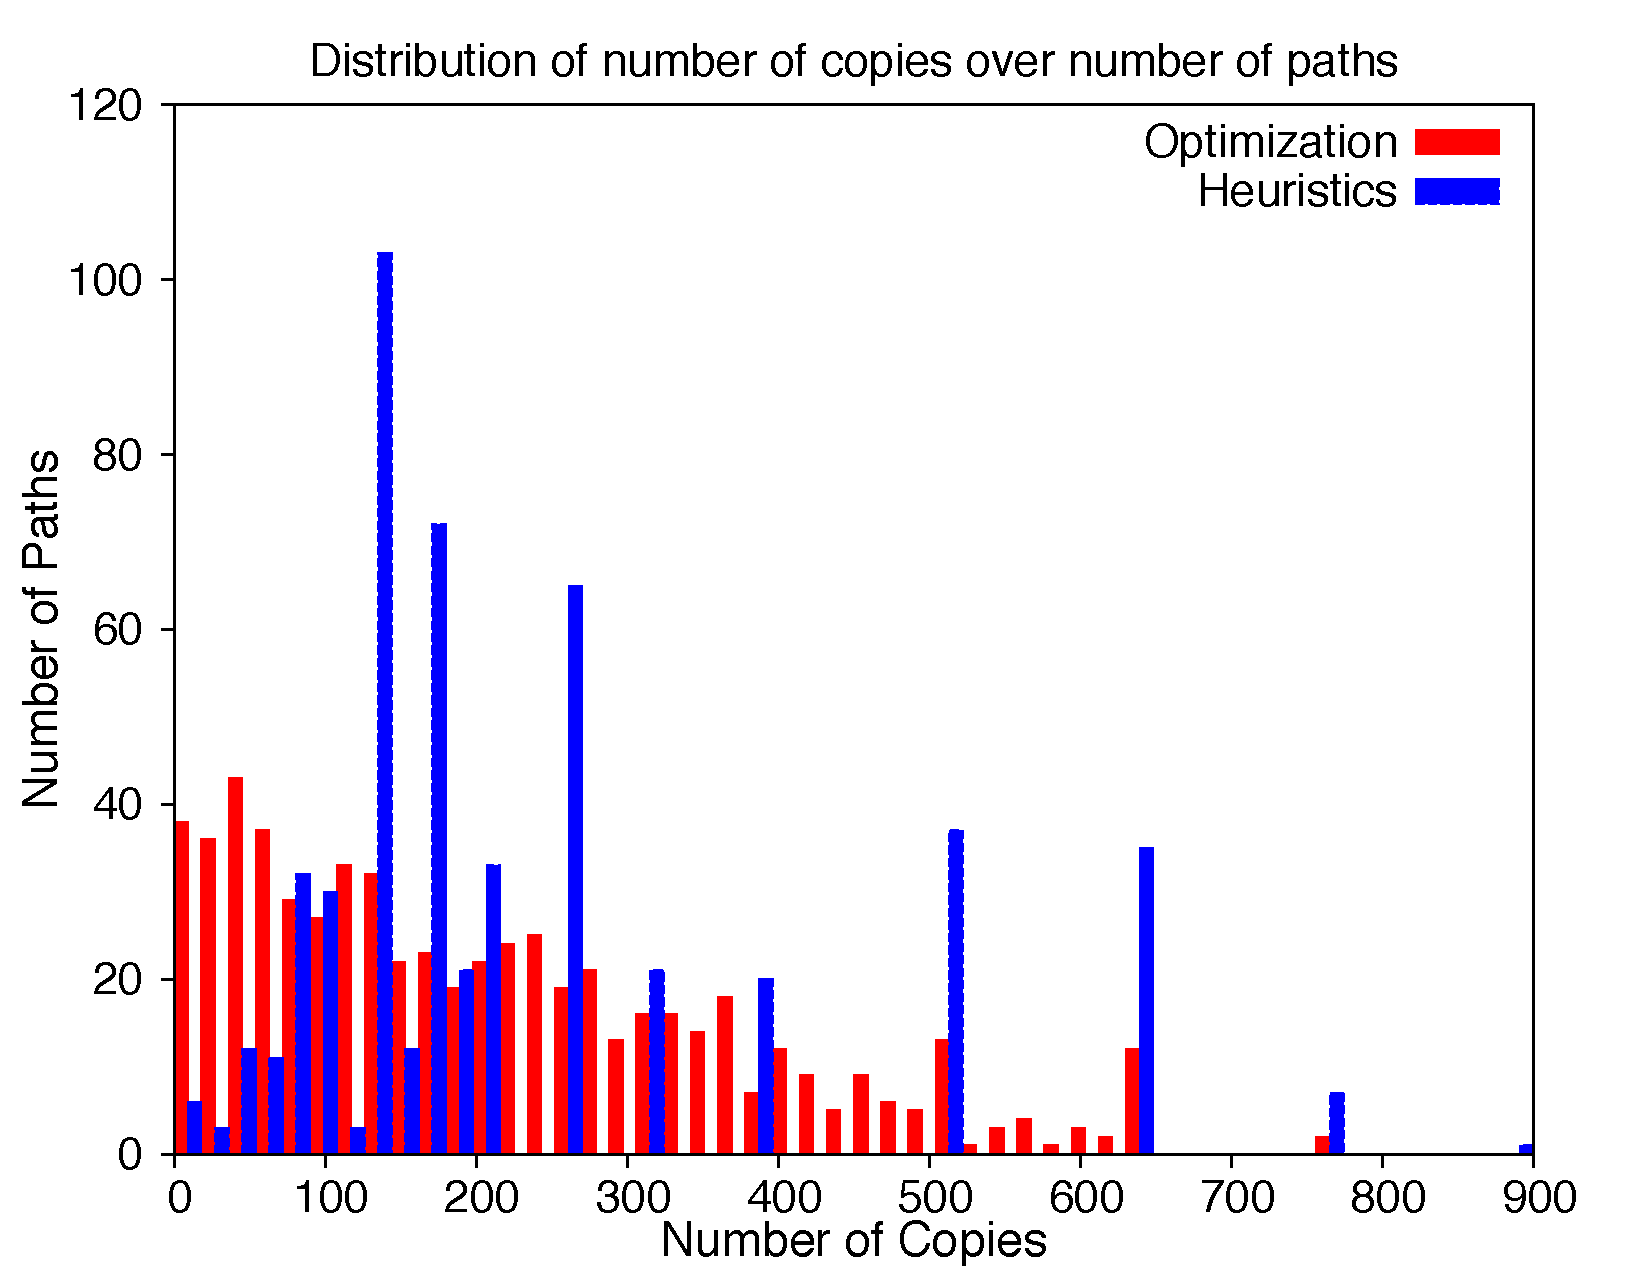
\includegraphics[width=\textwidth]{report_figures/hopcopy_histo.pdf}
                \caption{Distribution of number of copies over paths}
                \label{fig:512_hopcopy}
        \end{subfigure}
        \caption{Historgram of hops, copies, load in terms of number of paths and data size}
	\label{fig:512_histo}
\end{figure}

\clearpage
\newpage

\subsubsection{Total number of nodes 1024}

\input{tables/tables_87_1024.dat}

\begin{figure}[!htbp]
        \centering
        \begin{subfigure}[b]{0.49\textwidth}
                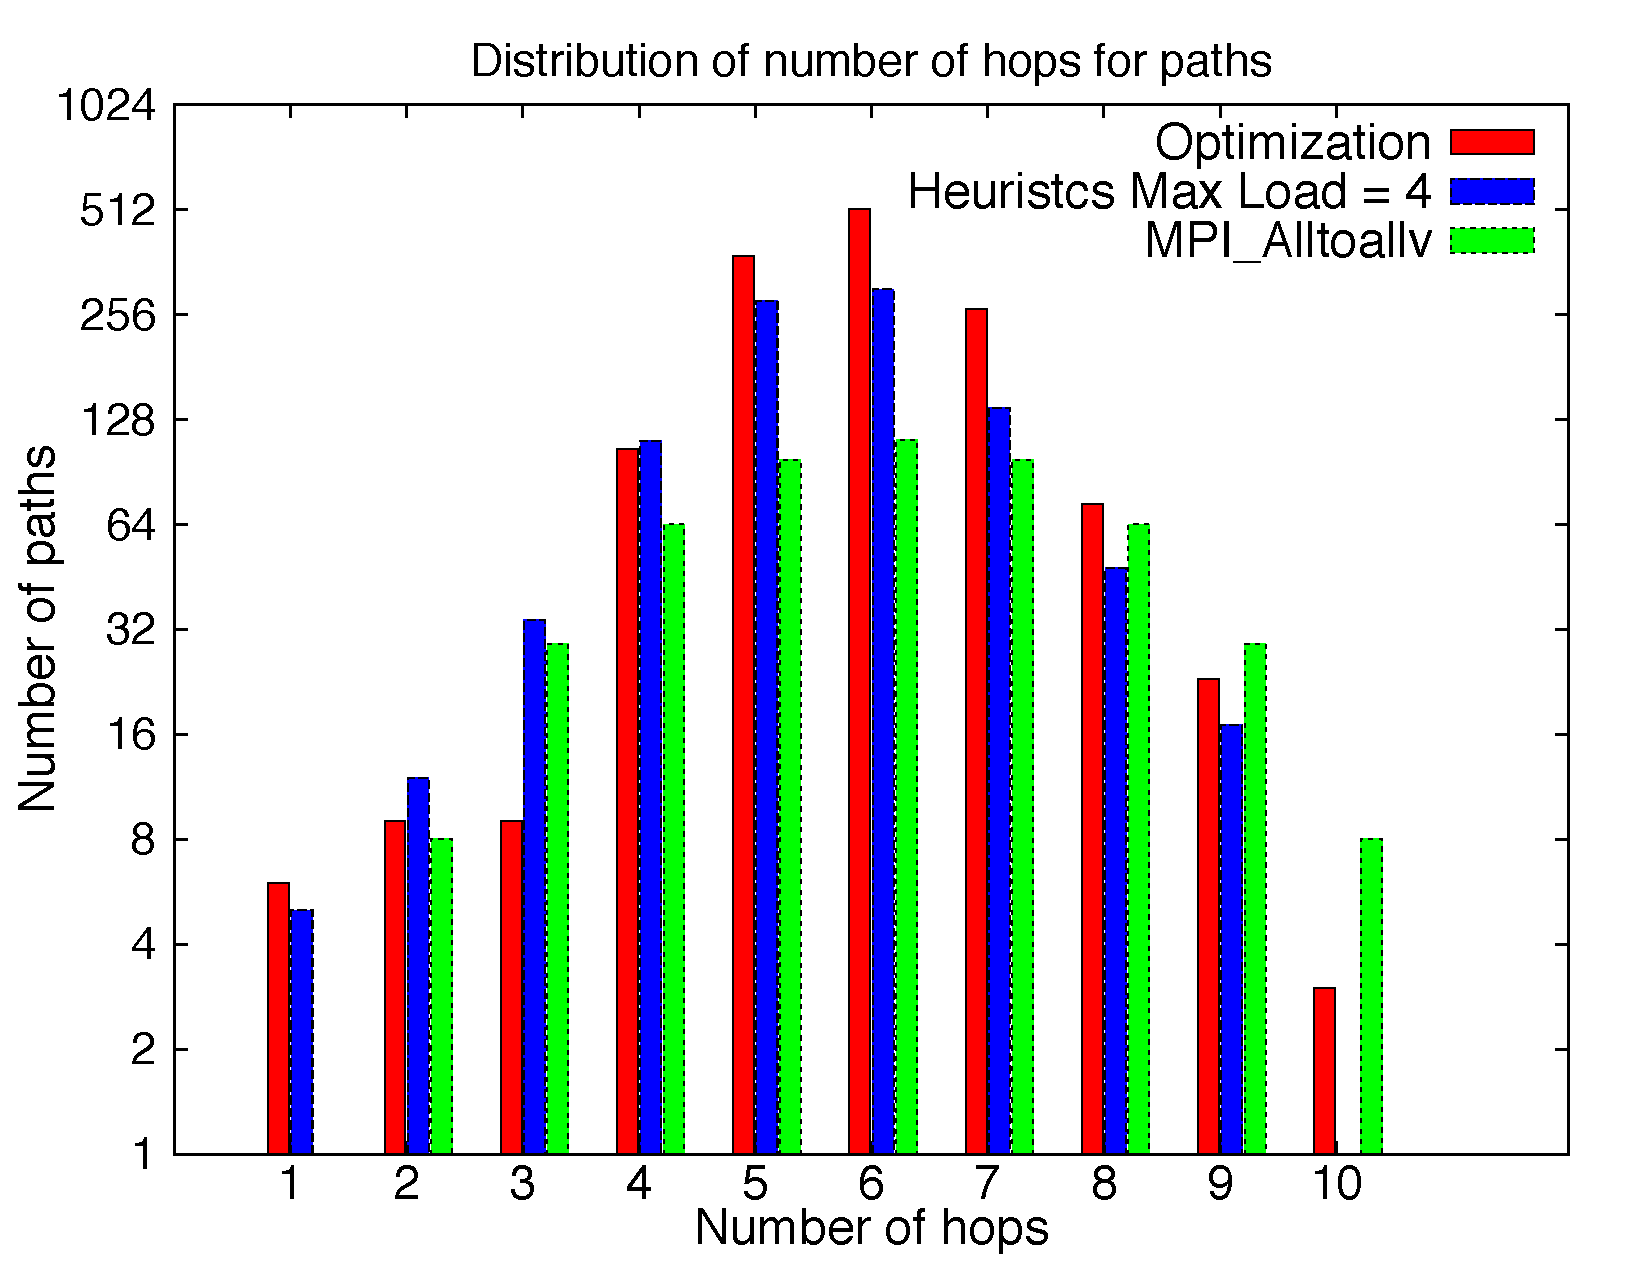
\includegraphics[width=\textwidth]{report_figures/1k/hop_histo.pdf}
                \caption{Distribution of number of hops over paths}
                \label{fig:1k_hop}
        \end{subfigure}%
        ~ %add desired spacing between images, e. g. ~, \quad, \qquad, \hfill etc.
          %(or a blank line to force the subfigure onto a new line)
        \begin{subfigure}[b]{0.49\textwidth}
                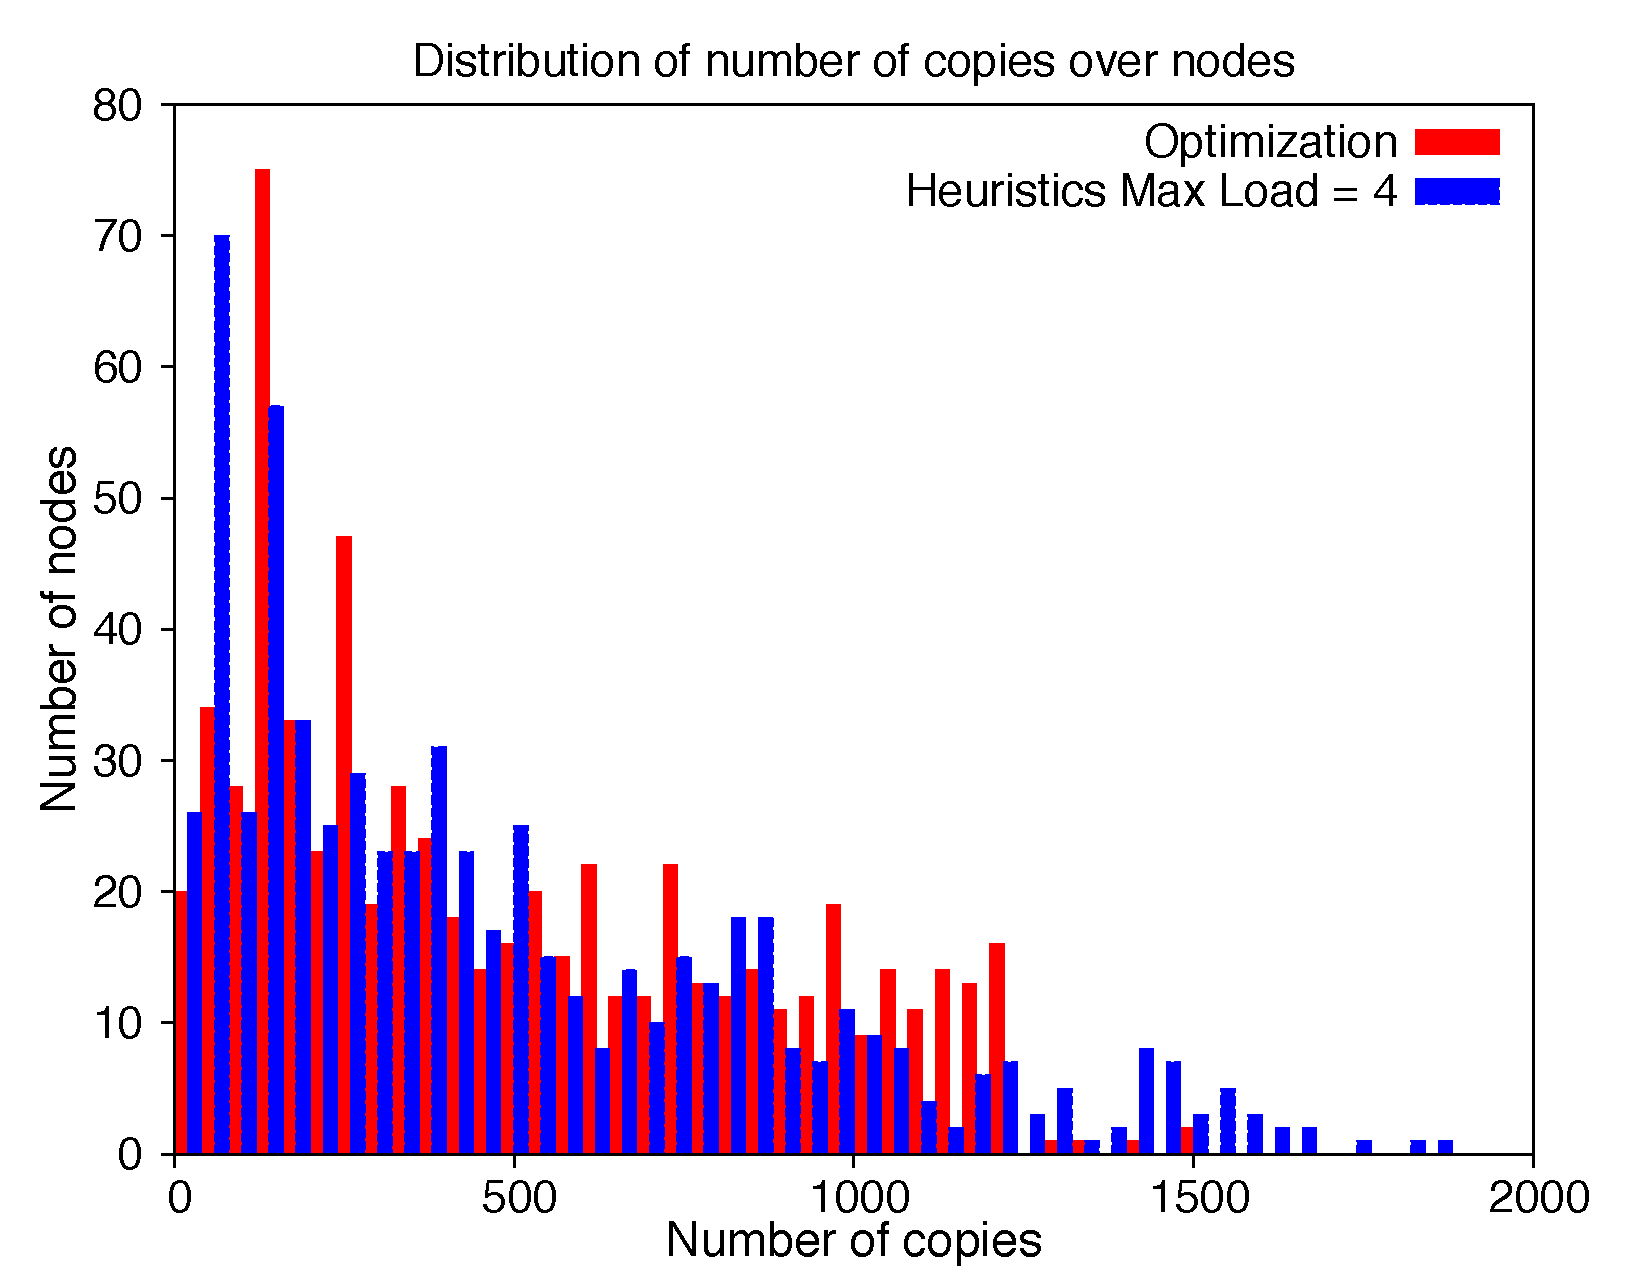
\includegraphics[width=\textwidth]{report_figures/1k/copy_histo.pdf}
                \caption{Distribution of number of copies over nodes}
                \label{fig:1k_copy}
        \end{subfigure}
        ~ %add desired spacing between images, e. g. ~, \quad, \qquad, \hfill etc.
          %(or a blank line to force the subfigure onto a new line)
        \begin{subfigure}[b]{0.49\textwidth}
                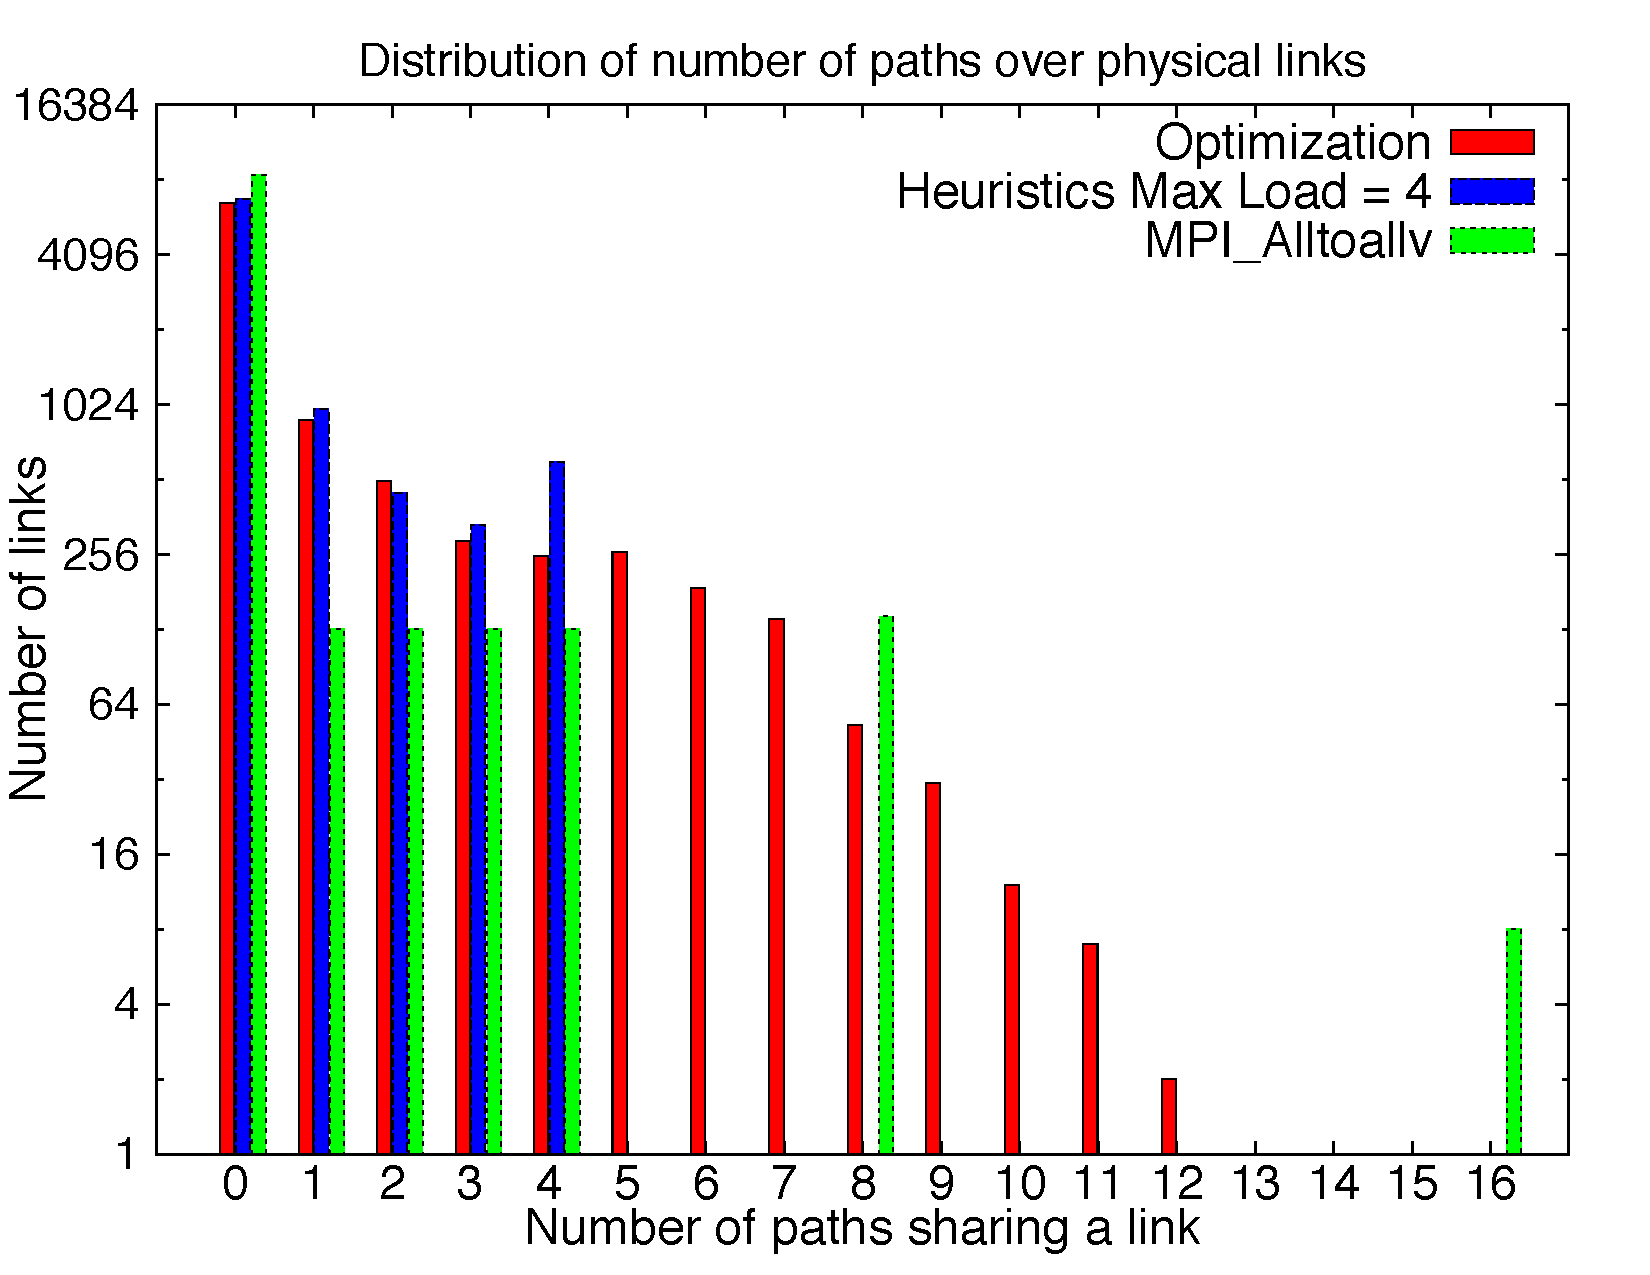
\includegraphics[width=\textwidth]{report_figures/1k/loadpath_histo.pdf}
                \caption{Distribution of number of paths over physicallinks}
                \label{fig:1k_loadpath}
        \end{subfigure}
        ~ %add desired spacing between images, e. g. ~, \quad, \qquad, \hfill etc.
          %(or a blank line to force the subfigure onto a new line)
        \begin{subfigure}[b]{0.49\textwidth}
                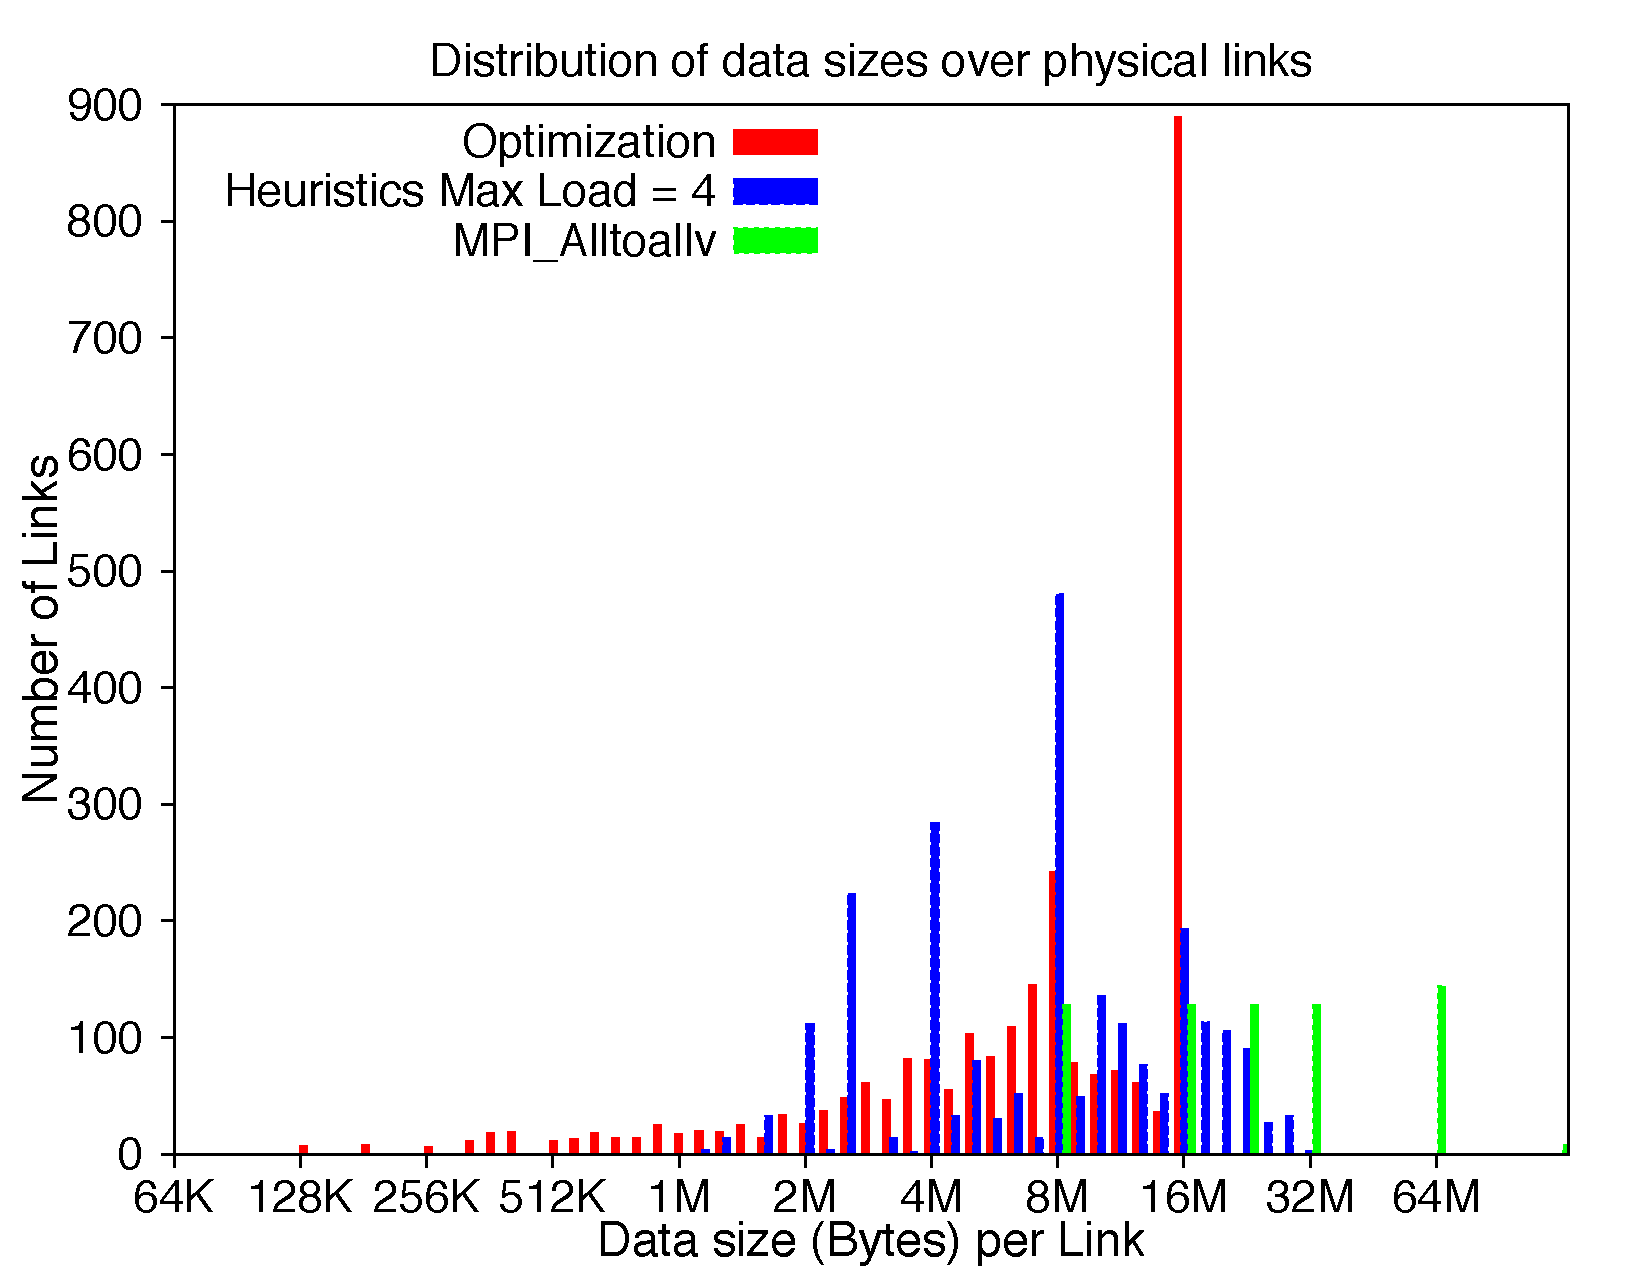
\includegraphics[width=\textwidth]{report_figures/1k/loaddata_histo.pdf}
                \caption{Distribution of total data size over physical links}
                \label{fig:1k_loaddata}
        \end{subfigure}
        ~ %add desired spacing between images, e. g. ~, \quad, \qquad, \hfill etc.
          %(or a blank line to force the subfigure onto a new line)
        \begin{subfigure}[b]{0.49\textwidth}
                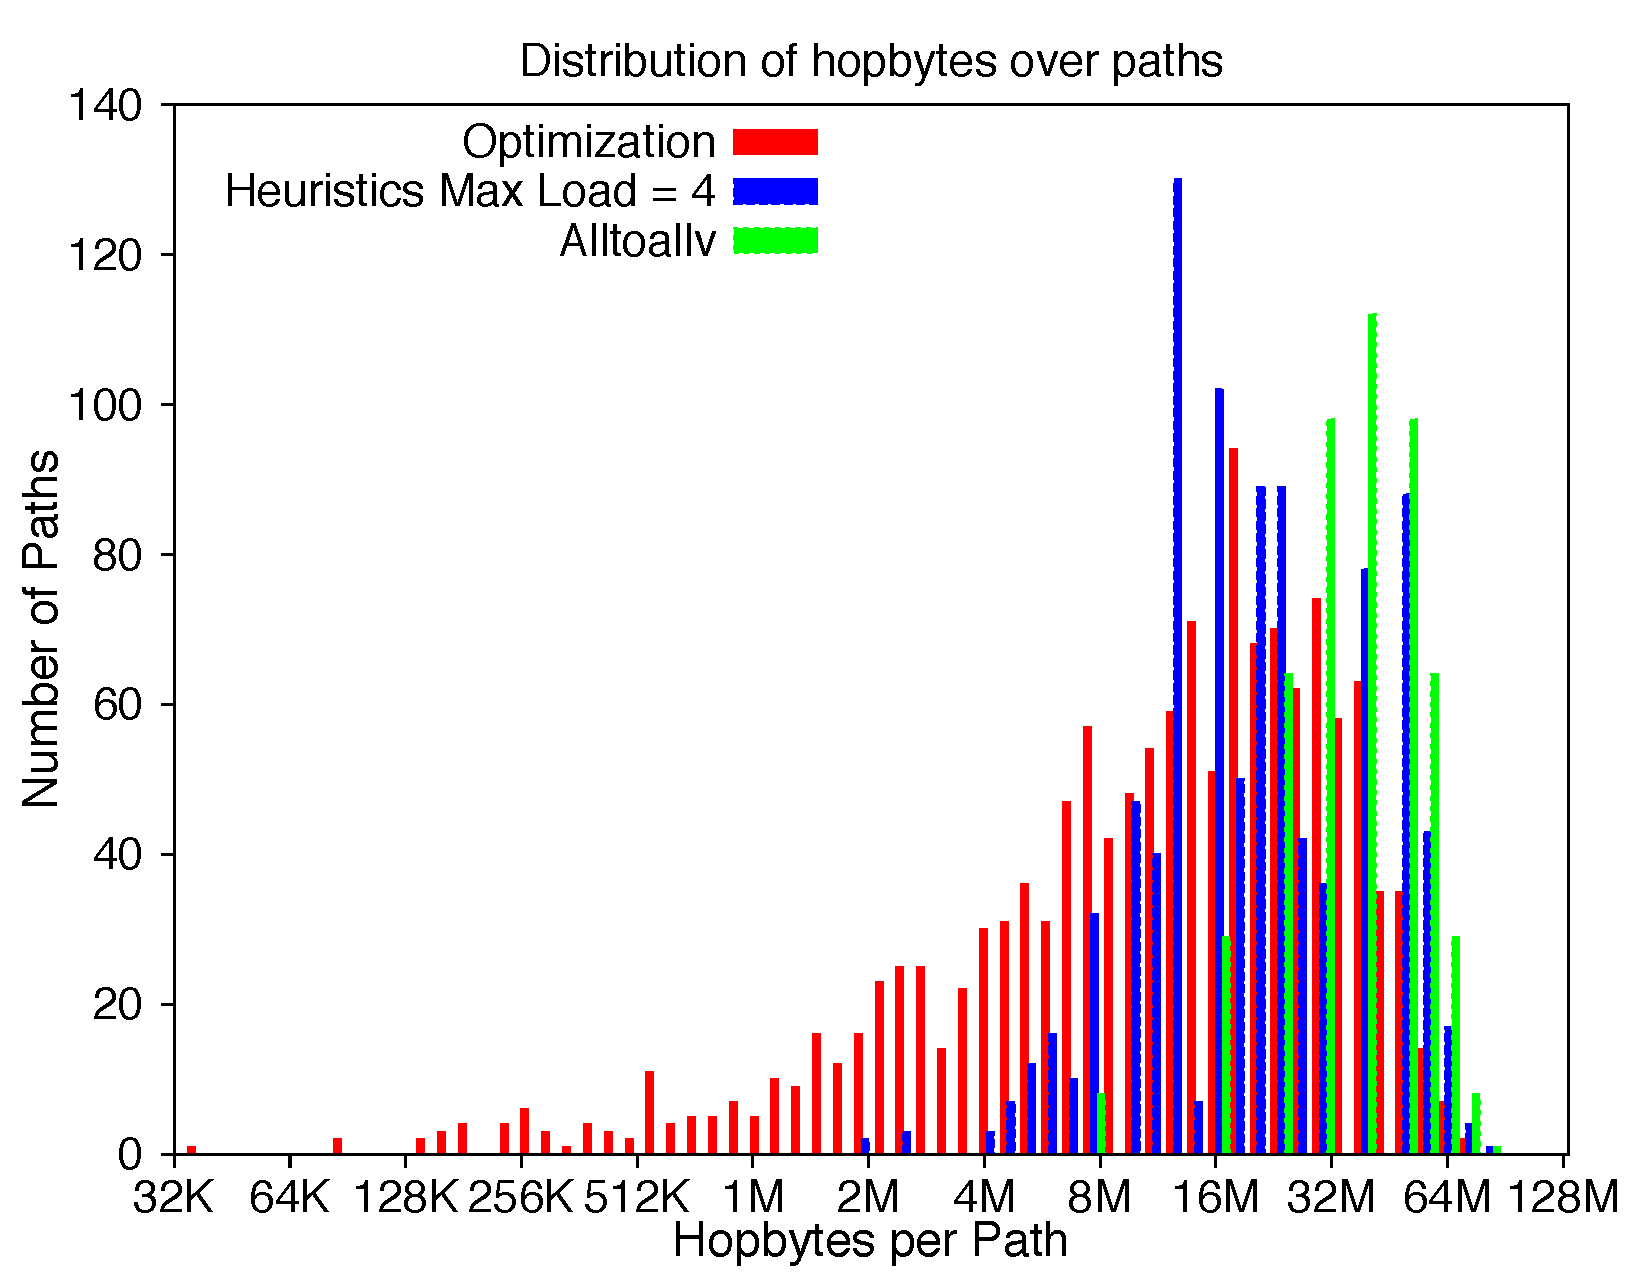
\includegraphics[width=\textwidth]{report_figures/1k/hopbyte_histo.pdf}
                \caption{Distribution of hopbytes over paths}
                \label{fig:1k_hopbyte}
        \end{subfigure}
        ~ %add desired spacing between images, e. g. ~, \quad, \qquad, \hfill etc.
          %(or a blank line to force the subfigure onto a new line)
        \begin{subfigure}[b]{0.49\textwidth}
                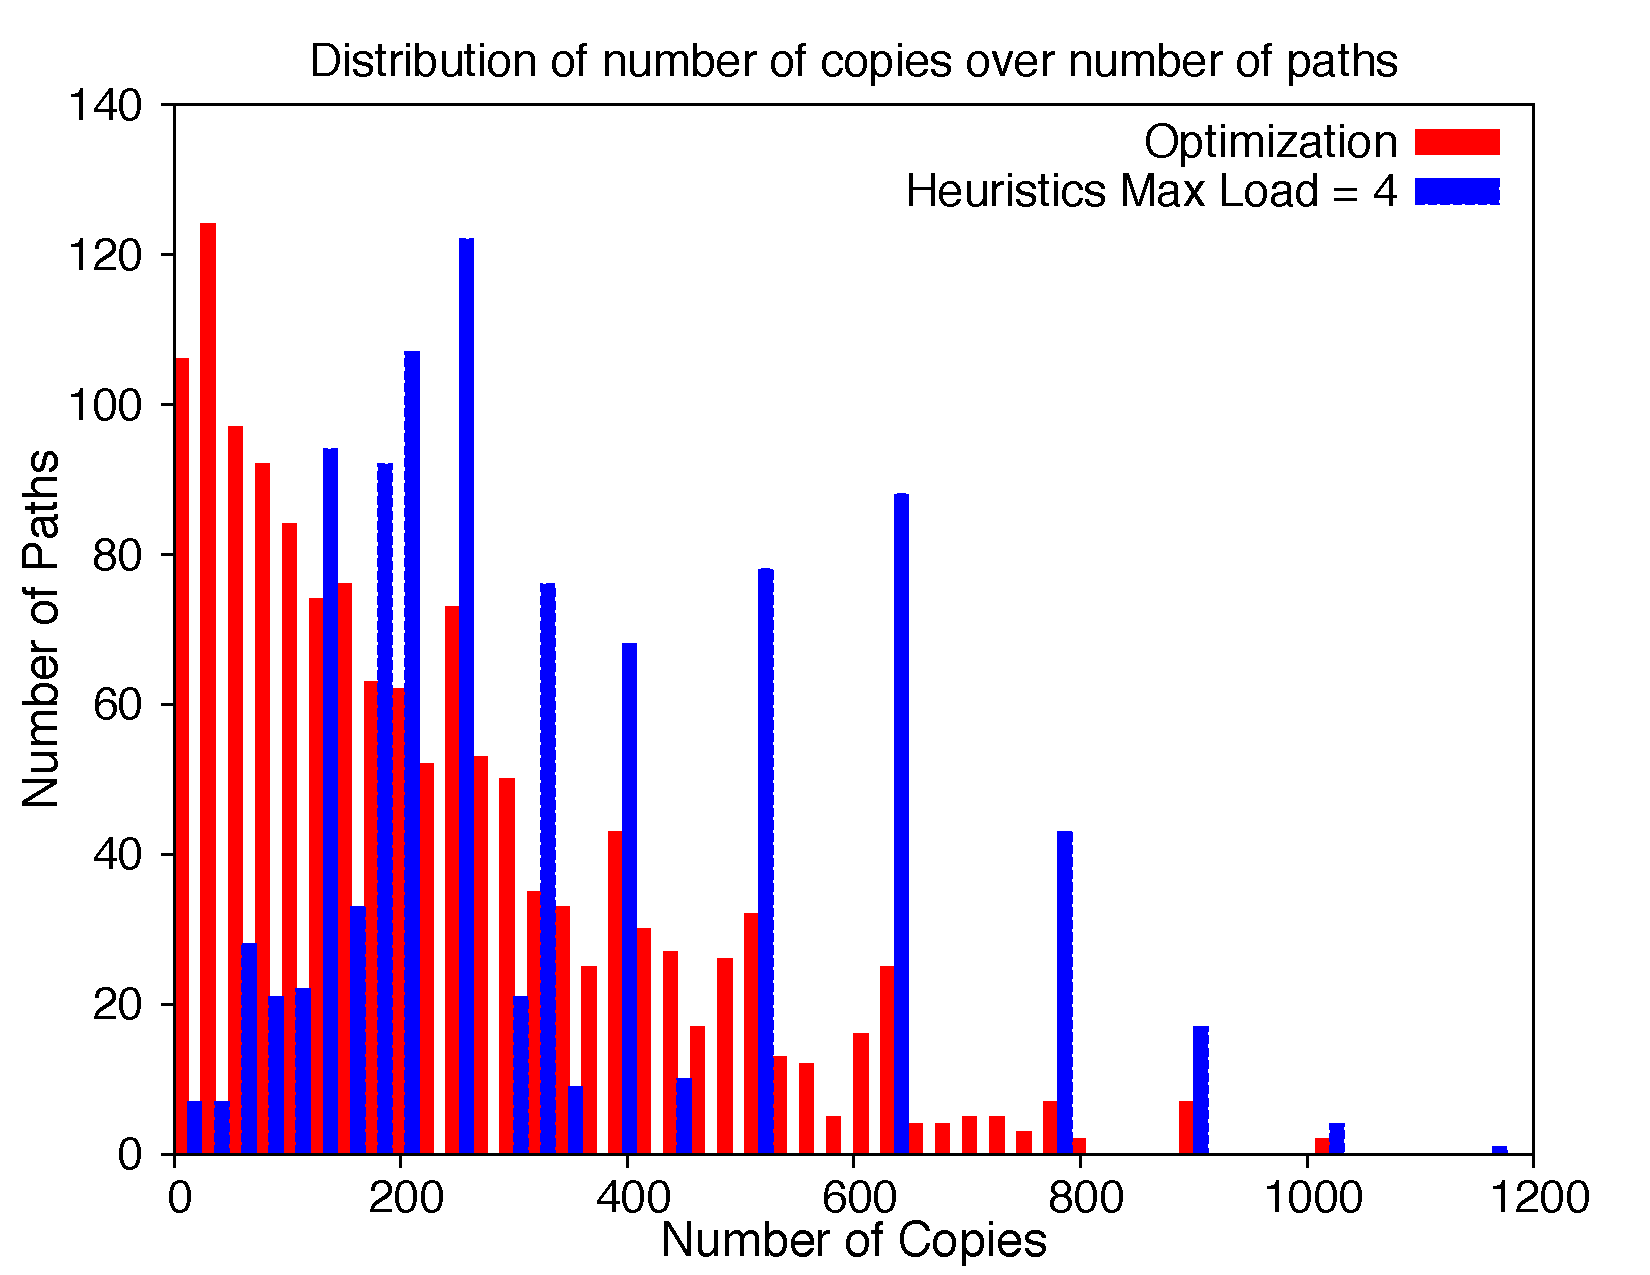
\includegraphics[width=\textwidth]{report_figures/1k/hopcopy_histo.pdf}
                \caption{Distribution of number of copies over paths}
                \label{fig:1k_hopcopy}
        \end{subfigure}
        \caption{Historgram of hops, copies, load in terms of number of paths and data size - 1K nodes}
        \label{fig:1k_histo}
\end{figure}

\clearpage
\newpage

\subsubsection {Total number of nodes 2048}

\input{tables/tables_87_2048.dat}

\begin{figure}[!htbp]
        \centering
        \begin{subfigure}[b]{0.49\textwidth}
                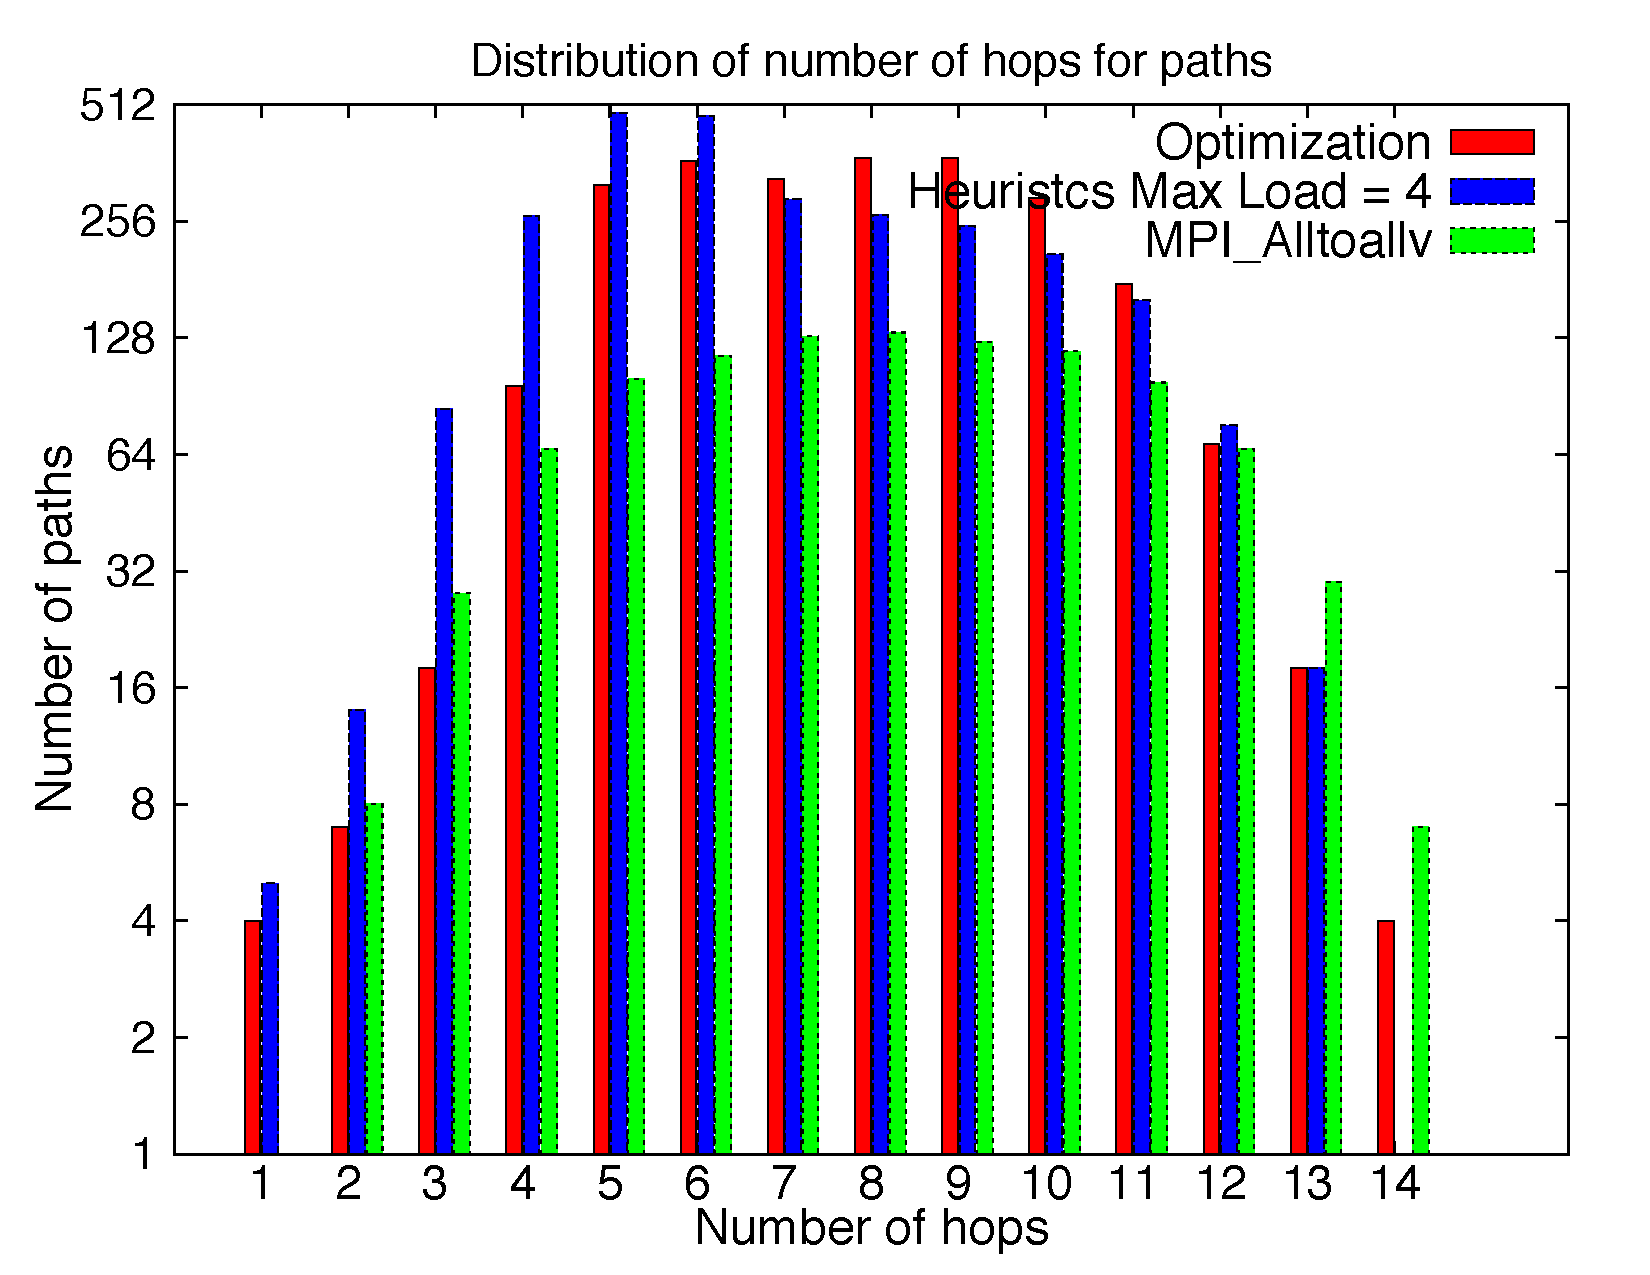
\includegraphics[width=\textwidth]{report_figures/2k/hop_histo.pdf}
                \caption{Distribution of number of hops over paths}
                \label{fig:2k_hop}
        \end{subfigure}%
        ~ %add desired spacing between images, e. g. ~, \quad, \qquad, \hfill etc.
          %(or a blank line to force the subfigure onto a new line)
        \begin{subfigure}[b]{0.49\textwidth}
                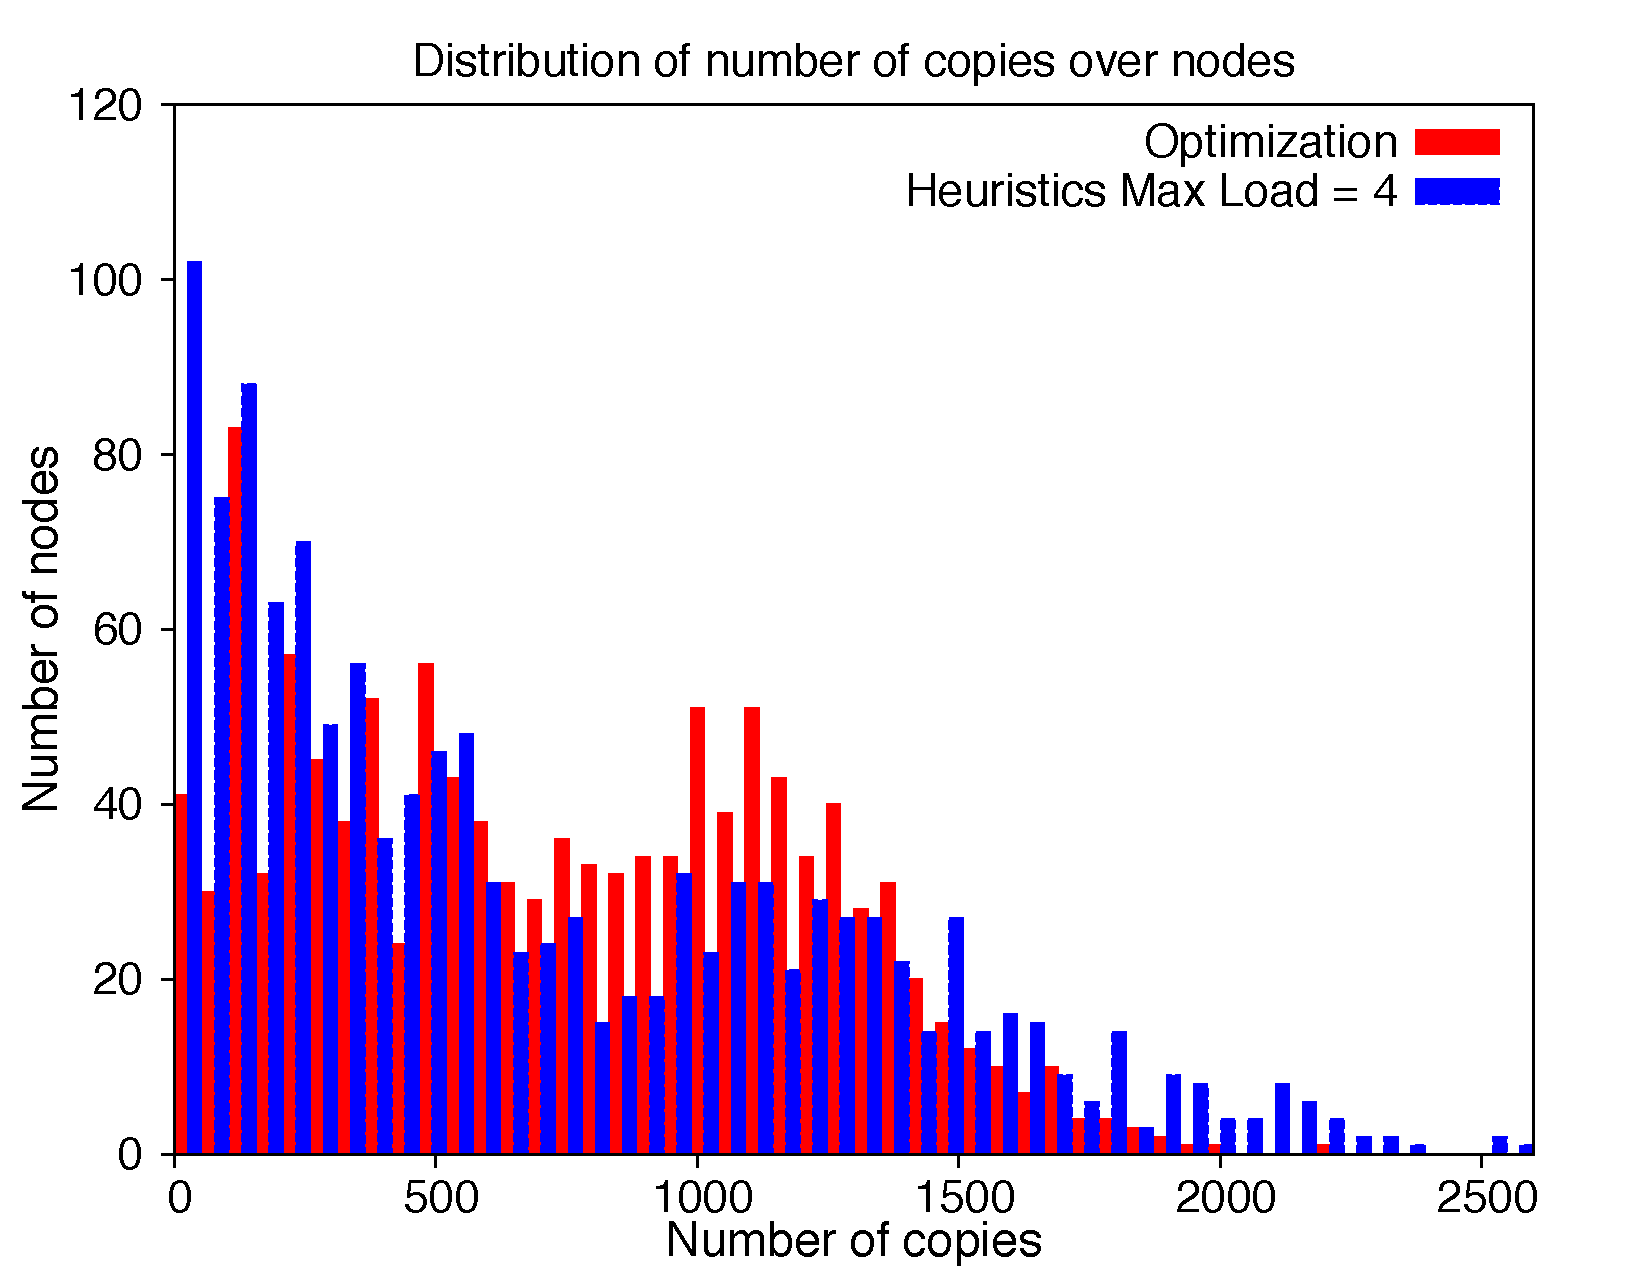
\includegraphics[width=\textwidth]{report_figures/2k/copy_histo.pdf}
                \caption{Distribution of number of copies over nodes}
                \label{fig:2k_copy}
        \end{subfigure}
        ~ %add desired spacing between images, e. g. ~, \quad, \qquad, \hfill etc.
          %(or a blank line to force the subfigure onto a new line)
        \begin{subfigure}[b]{0.49\textwidth}
                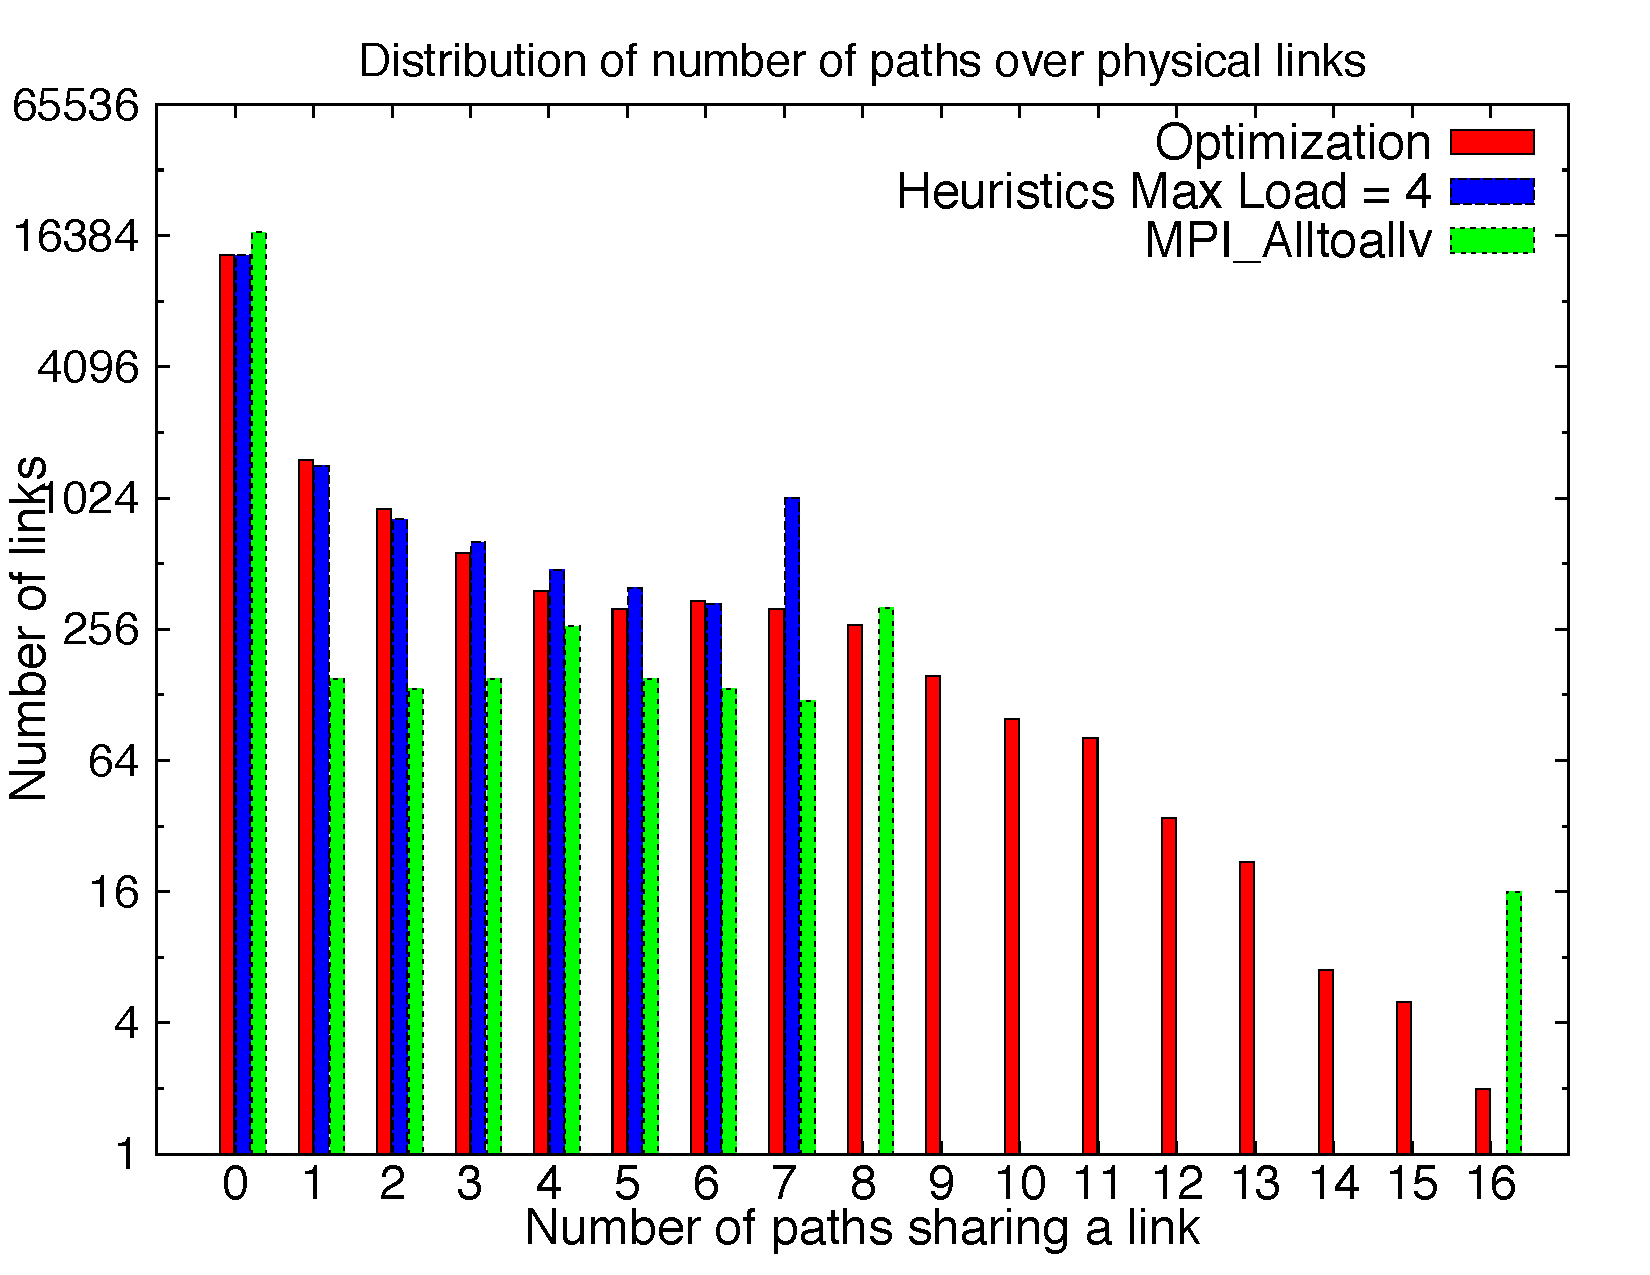
\includegraphics[width=\textwidth]{report_figures/2k/loadpath_histo.pdf}
                \caption{Distribution of number of paths over physicallinks}
                \label{fig:2k_loadpath}
        \end{subfigure}
        ~ %add desired spacing between images, e. g. ~, \quad, \qquad, \hfill etc.
          %(or a blank line to force the subfigure onto a new line)
        \begin{subfigure}[b]{0.49\textwidth}
                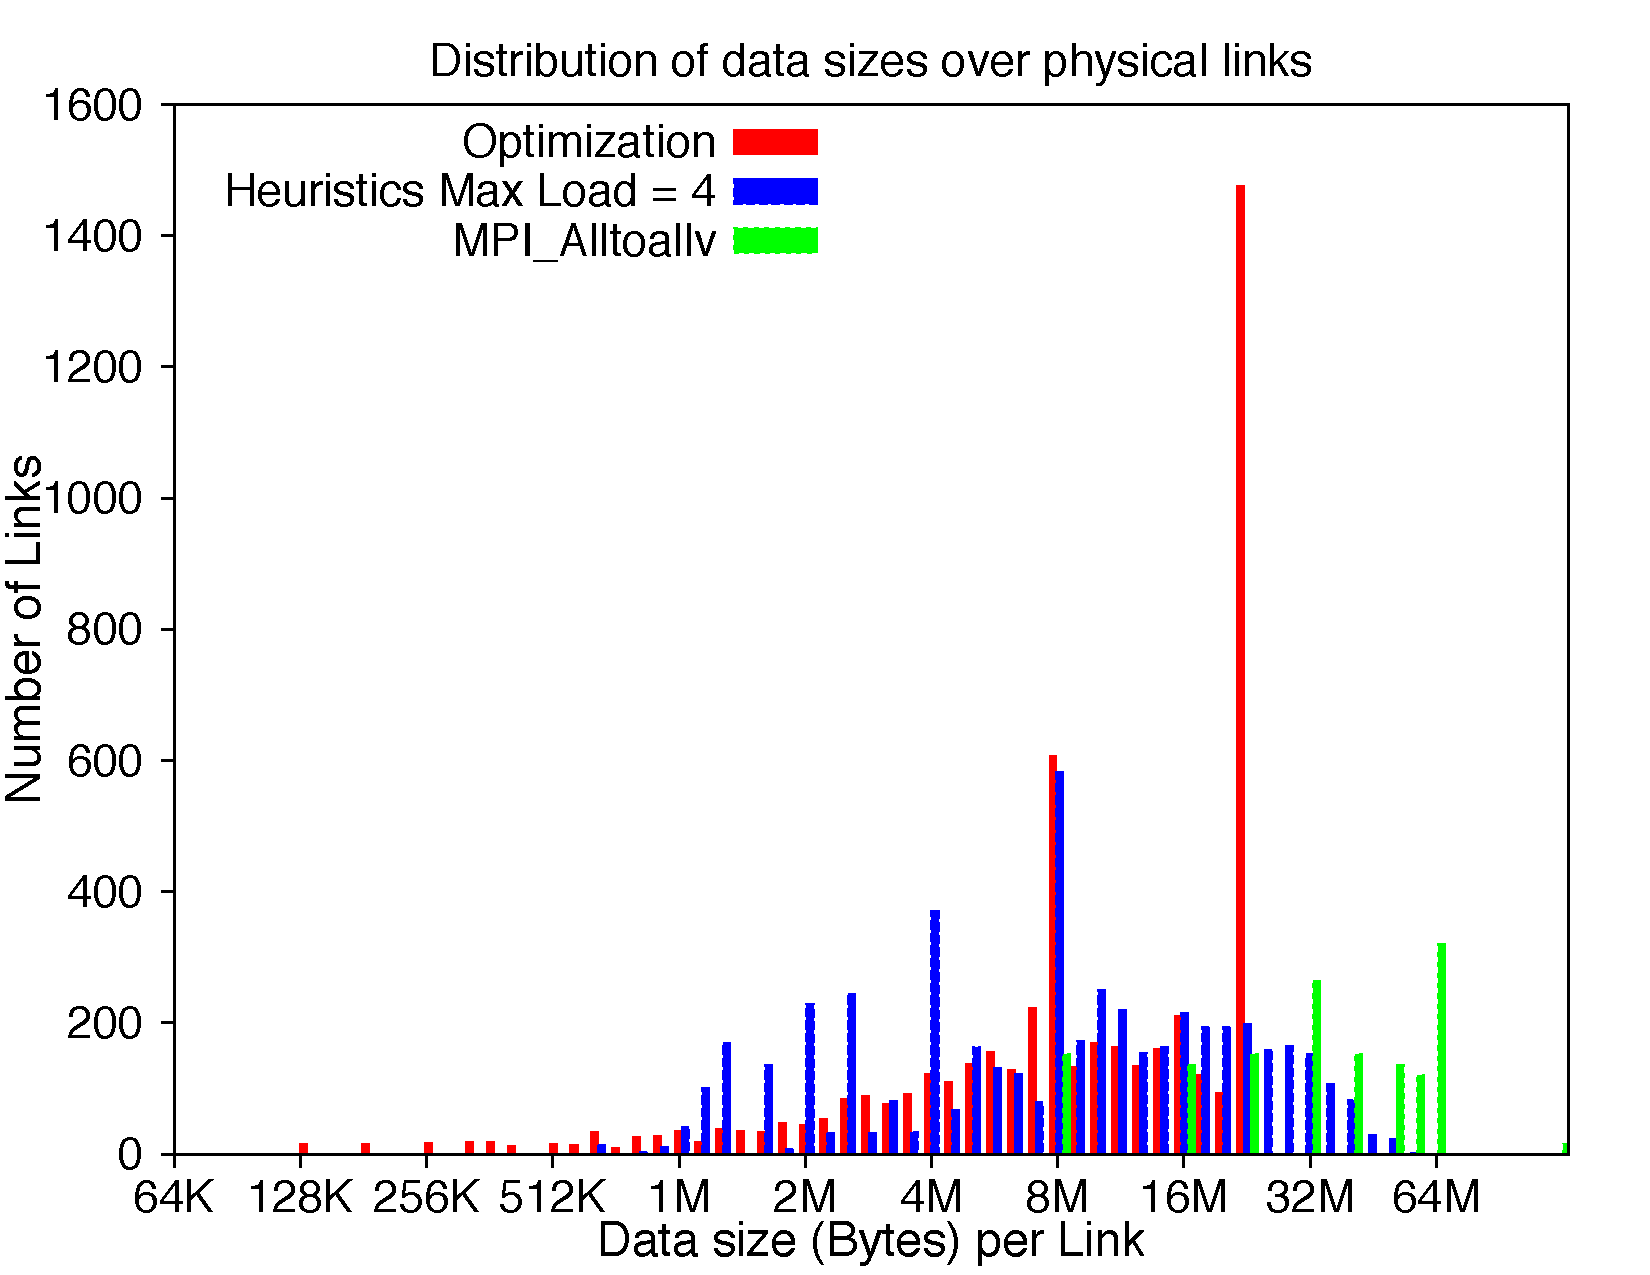
\includegraphics[width=\textwidth]{report_figures/2k/loaddata_histo.pdf}
                \caption{Distribution of total data size over physical links}
                \label{fig:2k_loaddata}
        \end{subfigure}
        ~ %add desired spacing between images, e. g. ~, \quad, \qquad, \hfill etc.
          %(or a blank line to force the subfigure onto a new line)
        \begin{subfigure}[b]{0.49\textwidth}
                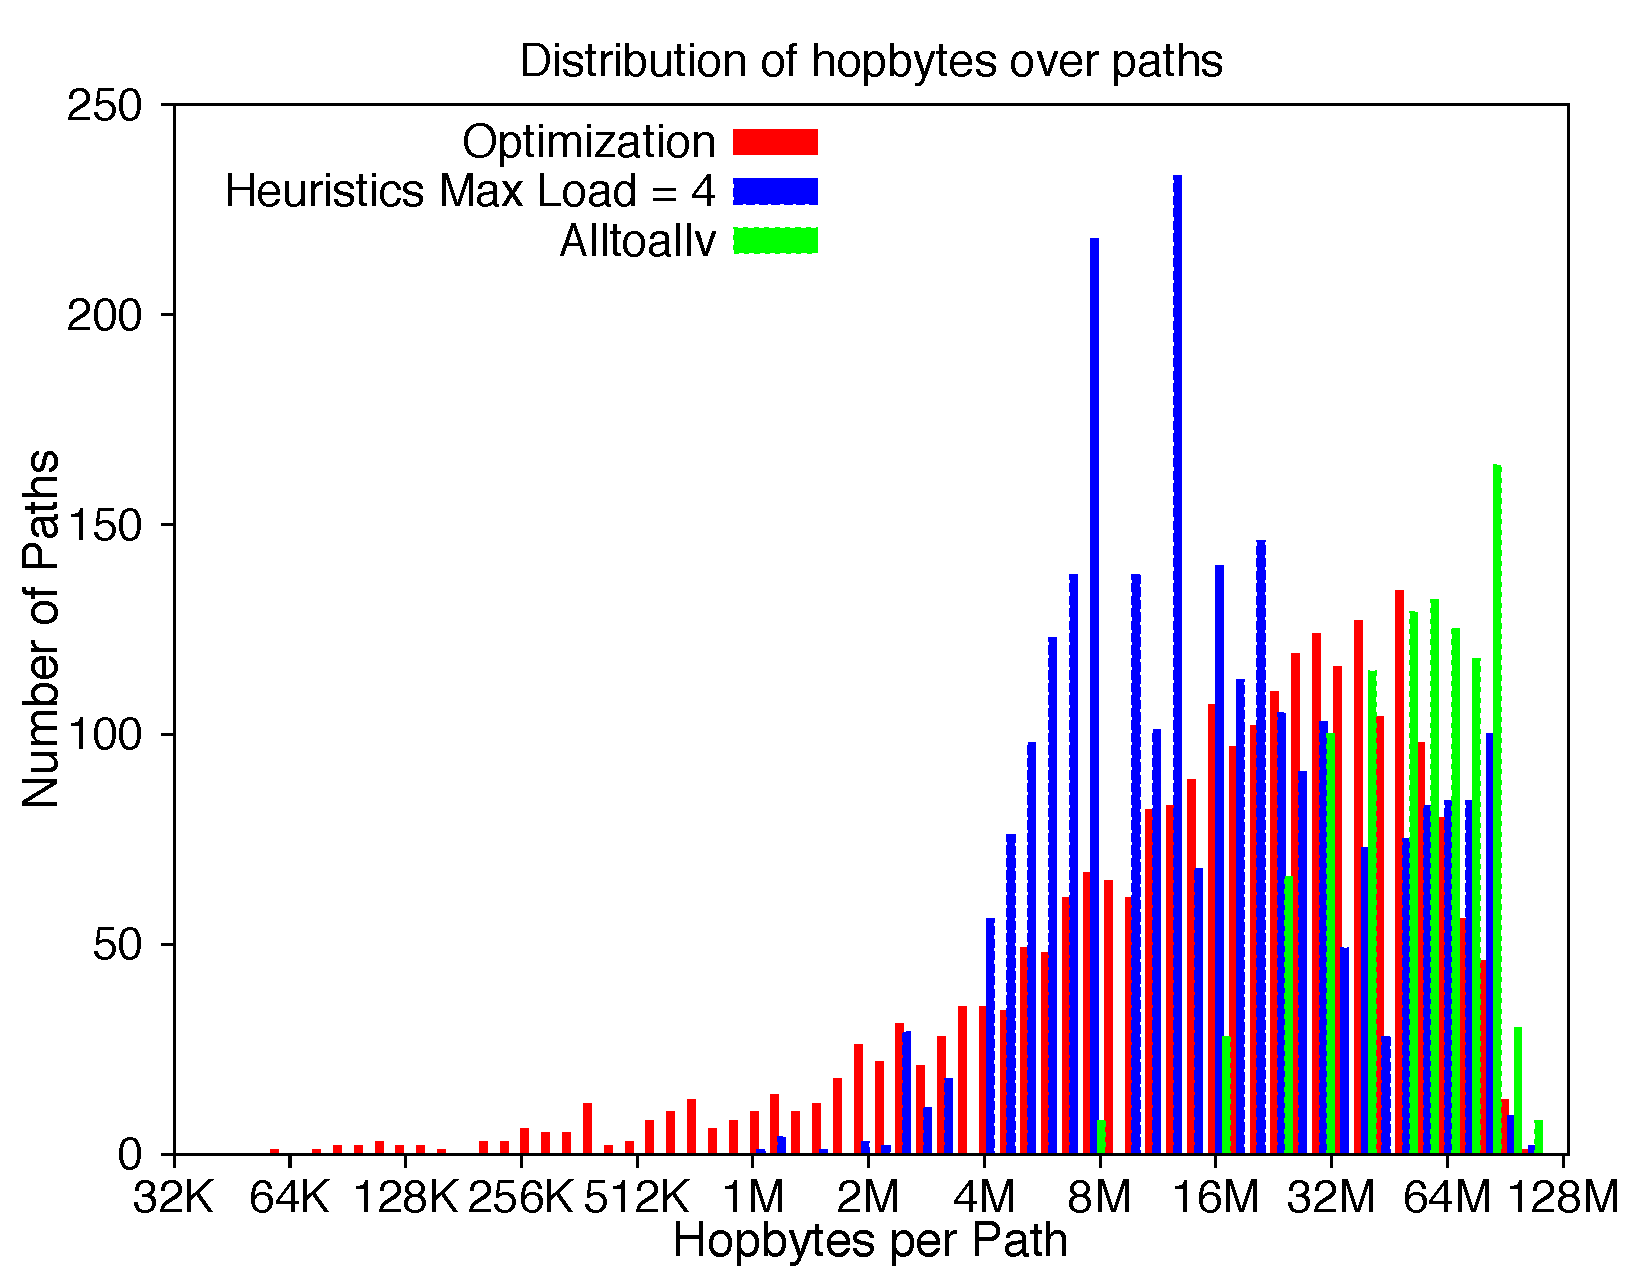
\includegraphics[width=\textwidth]{report_figures/2k/hopbyte_histo.pdf}
                \caption{Distribution of hopbytes over paths}
                \label{fig:2k_hopbyte}
        \end{subfigure}
        ~ %add desired spacing between images, e. g. ~, \quad, \qquad, \hfill etc.
          %(or a blank line to force the subfigure onto a new line)
        \begin{subfigure}[b]{0.49\textwidth}
                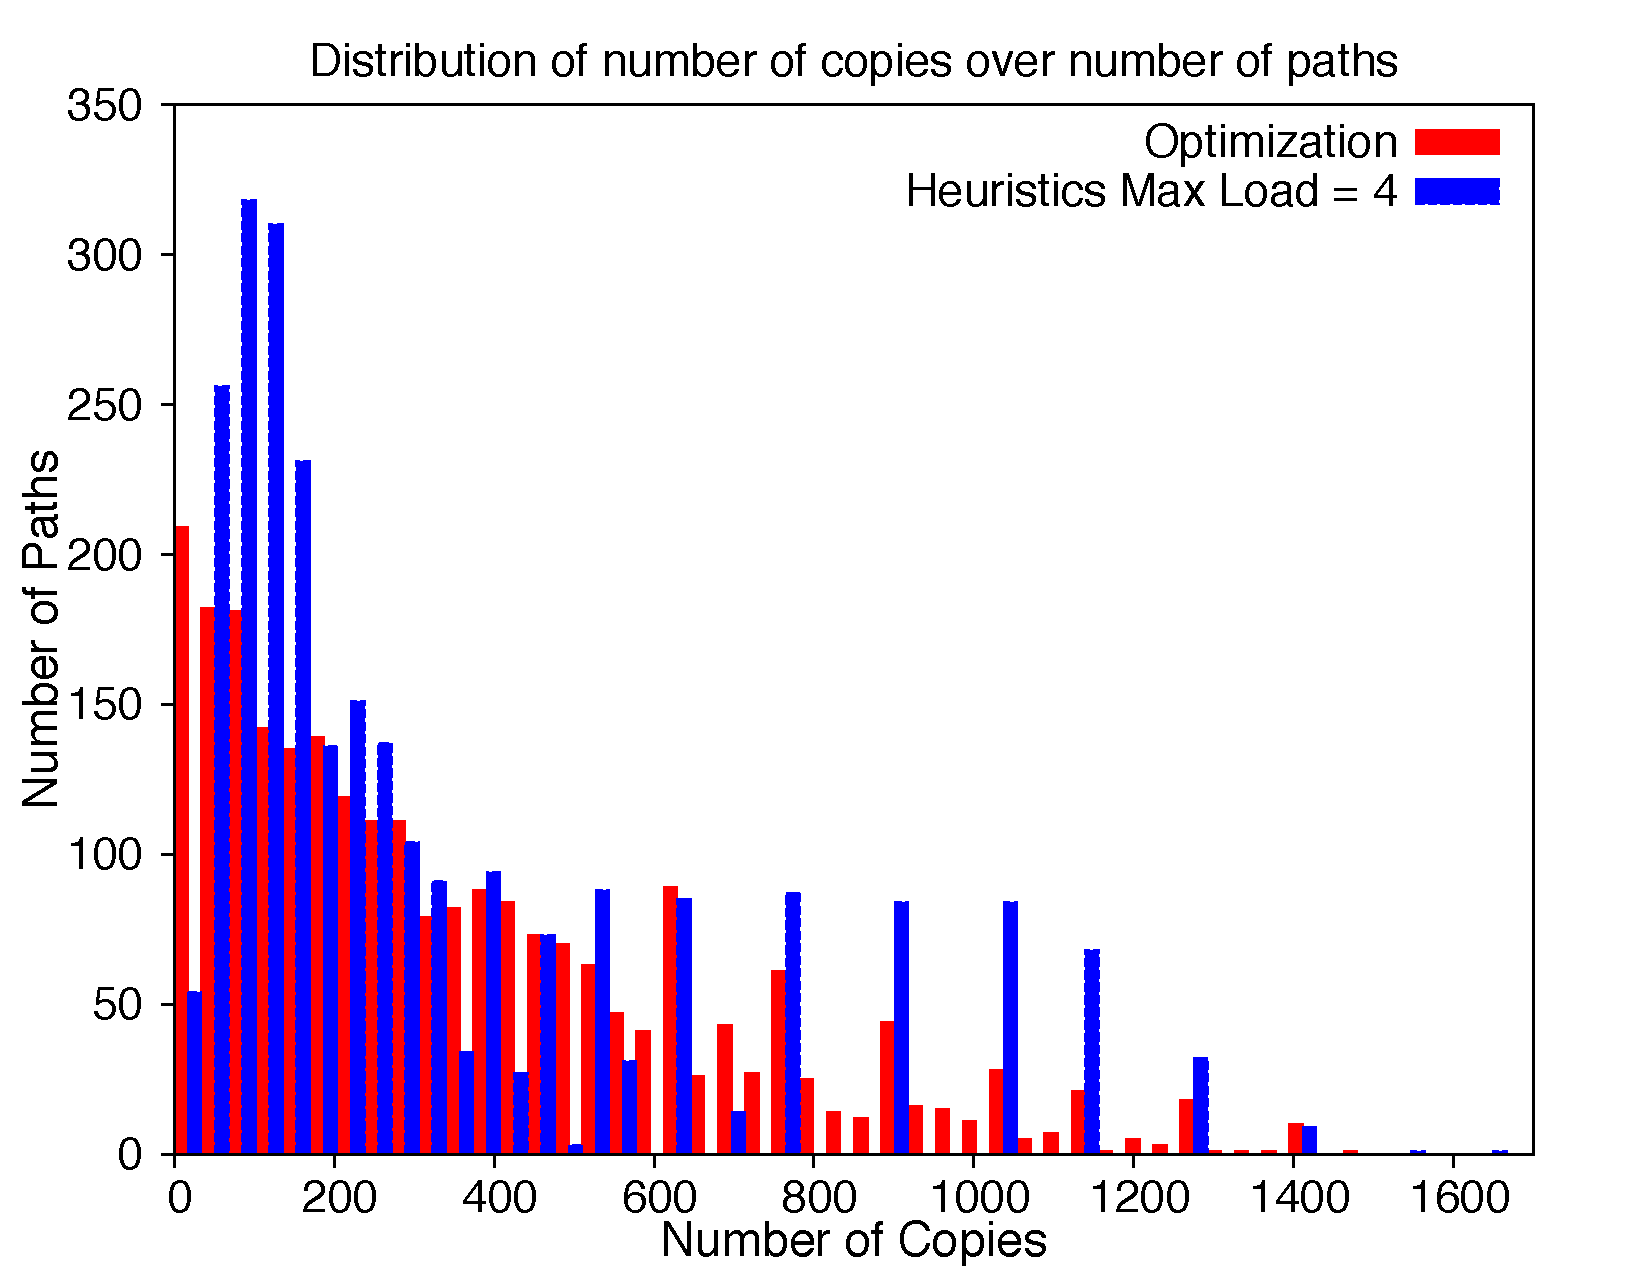
\includegraphics[width=\textwidth]{report_figures/2k/hopcopy_histo.pdf}
                \caption{Distribution of number of copies over paths}
                \label{fig:2k_hopcopy}
        \end{subfigure}
        \caption{Historgram of hops, copies, load in terms of number of paths and data size - 2K nodes}
        \label{fig:2k_histo}
\end{figure}

\clearpage
\newpage

\subsubsection {Total number of nodes 4096}

\input{tables/tables_87_4096.dat}

\clearpage
\newpage

\section{First 128 to 256}

\section {Increasing distance between sources and destinations}

\subsection{Total nodes of 2048}

Number of sources is 256. Sources are [0-256]. Number of destinations is 512. As the destinations move further from the sources, the performance increases.

\begin{figure}[h]
\vspace{-0.1in}
\centering
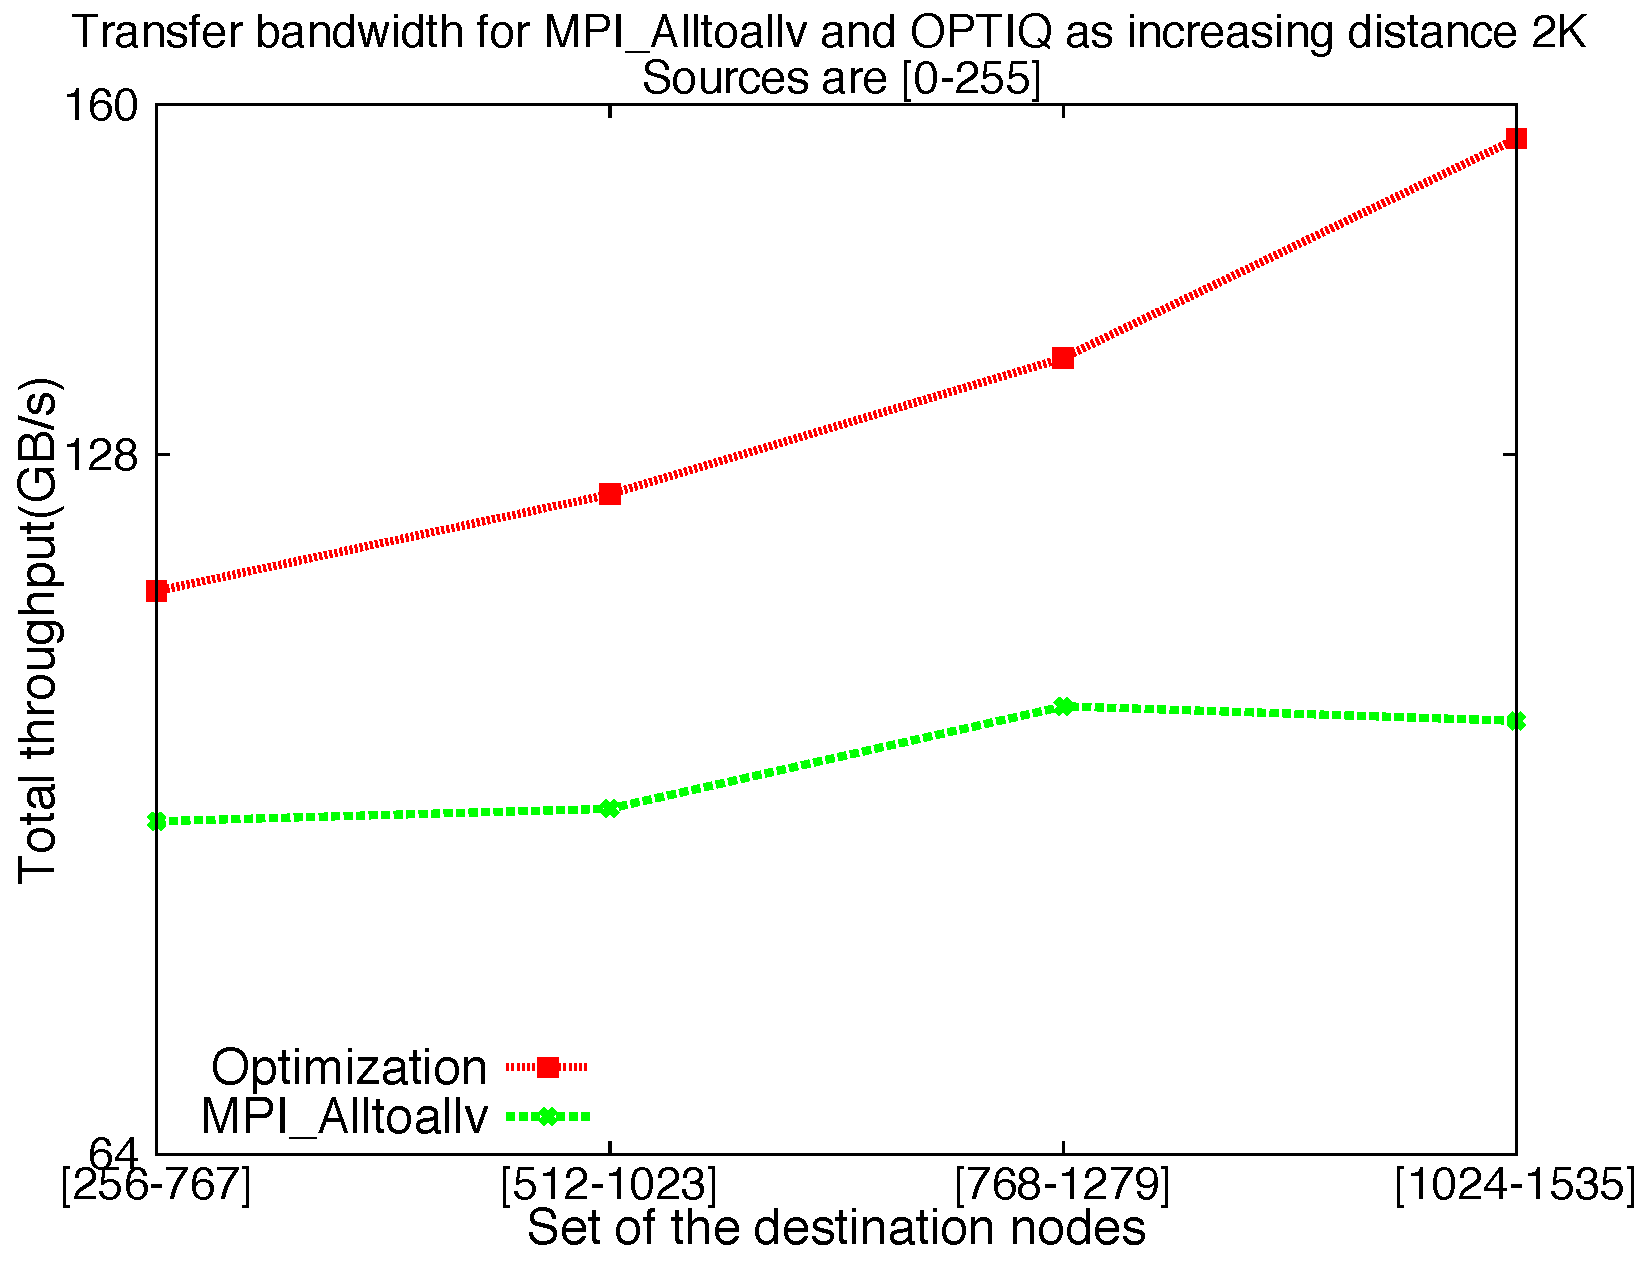
\includegraphics[scale=0.40]{report_figures/incrdist/incrdist_2k.pdf}
\vspace{-0.1in}
\caption{Increasing distance}
\vspace{-0.1in}
\label{fig:incrdist_2k}
\end{figure}

\clearpage
\newpage

\begin{table}[!htbp]
   \centering
    \begin{tabular}{ | l | p{0.75cm} | p{1.0cm} | p{1.0cm} | p{0.75cm} | p{0.5cm} | p{0.5cm} | p{0.5cm} | p{0.5cm} |}
    \hline
    \multirow{3}{*}{Destinations} & \multicolumn{3}{ c| }{Performance} & \multicolumn{5}{ c| }{Num. of Paths} \\ \cline{2-9}
    & Data (MB) & Time ($\mu$s) & BW (MB/s)& \multirow{2}{1cm}{Total Paths} & \multicolumn{4}{ c| }{Per Job} \\ \cline{6-9}
    & & & & & Max & Min & Avg & Med \\ \hline
    256-767 & 4096  & 34632 & 118272 & 1105 & 6 & 1 & 2.16 & 2 \\ \hline
    512-1023 & 4096  & 32167 & 127335 & 1372 & 7 & 1 & 2.68 & 3 \\ \hline
    768-1279 & 4096  & 29235 & 140106 & 1547 & 7 & 1 & 3.02 & 3 \\ \hline
    1024-1535 & 4096  & 25499 & 160633 & 1672 & 8 & 1 & 3.27 & 3 \\ \hline
    \end{tabular}
    \caption{Performance with number of paths in 2048 nodes experiments}
    \label{table:2048_perf}
\end{table}


\begin{table}[!htbp]
    \centering
    \begin{tabular}{ | l | p{0.75cm} | p{0.5cm} | p{0.5cm} | p{0.5cm} | p{0.5cm} | p{1.0cm} | p{0.75cm} | p{0.5cm} | p{1.0cm} | p{0.5cm} |}
    \hline
    \multirow{3}{*}{Destinations} & \multicolumn{5}{ c| }{Num. of Hops} & \multicolumn{5}{ c| }{Num. of Copies} \\ \cline{2-11}
    & \multirow{2}{1cm}{Total hops} & \multicolumn{4}{ c| }{Per Path} & \multirow{2}{1cm}{Total copies} & \multicolumn{4}{ c| }{Per Node} \\ \cline{3-6} \cline{8-11}
    & & Max & Min & Avg & Med & & Max & Min & Avg & Med \\ \hline
    256-767 &  8569 & 13 & 1 & 7.75 & 8 & 403937 & 1138 & 3 & 481.45 & 458 \\ \hline
    512-1023 &  11135 & 14 & 1 & 8.12 & 8 & 435057 & 1063 & 3 & 424.86 & 402 \\ \hline
    768-1279 &  15064 & 15 & 2 & 9.01 & 9 & 493197 & 786 & 1 & 269.80 & 242 \\ \hline
    1024-1535 &  15064 & 15 & 2 & 9.01 & 9 & 493197 & 786 & 1 & 269.80 & 242 \\ \hline
    \end{tabular}
    \caption{Number of hops and copies in 2048 nodes experiments}
    \label{table:2048_hopcopy}
\end{table}


\begin{table}[!htbp]
    \centering
    \begin{tabular}{ | l | p{2cm} | p{1.5cm} | p{1.0cm} | p{1.5cm} | p{1.5cm} | p{1.0cm} | p{0.75cm} | p{0.5cm} | p{1cm} | p{0.75cm} |}
    \hline
    \multirow{3}{*}{Destinations} & \multicolumn{5}{ c| }{Hopbytes} & \multicolumn{5}{ c| }{Num. of Copies} \\ \cline{2-11}
    & \multirow{2}{1cm}{Total hopbytes} & \multicolumn{4}{ c| }{Per Path} & \multirow{2}{1cm}{Total copies} & \multicolumn{4}{ c| }{Per Path} \\ \cline{3-6} \cline{8-11}
    & & Max & Min & Avg & Med & & Max & Min & Avg & Med \\ \hline
    256-767 &  30765113439 & 100663296 & 68432 & 27841731 & 25048499 & 403912 & 1408 & 6 & 365.53 & 306 \\ \hline
    512-1023 &  32804773165 & 117440512 & 64400 & 23910184 & 19321168 & 435032 & 1664 & 3 & 317.08 & 252 \\ \hline
    768-1279 &  34556080096 & 117440512 & 49128 & 22337479 & 18226488 & 461754 & 1664 & 5 & 298.48 & 246 \\ \hline
    1024-1535 &  36615449851 & 116415166 & 22516 & 21899192 & 17970760 & 493172 & 1638 & 3 & 294.96 & 235 \\ \hline
    \end{tabular}
    \caption{Number of hopbytes and copies per path in 2048 nodes experiments}
    \label{table:2048_hopbyte}
\end{table}

\begin{table}[!htbp]
    \centering
    \begin{tabular}{ | l | p{0.75cm} | p{0.5cm} | p{0.5cm} | p{0.5cm} | p{0.5cm} | p{1.5cm} | p{1.5cm} | p{1.25cm} | p{1.5cm} |}
    \hline
    \multirow{2}{*}{Destinations} & \multicolumn{5}{ c| }{Load (Num of Paths) per Link} & \multicolumn{4}{ c| }{Actual Load (Data Amount) per Link} \\ \cline{2-10}
    & Total & Max & Min & Avg & Med & Max & Min & Avg & Med \\ \hline
    256-767 &  1105 & 13 & 1 & 2.78 & 2 & 20447232 & 65536 & 9969456 & 8388608 \\ \hline
    512-1023 &  1372 & 13 & 1 & 2.85 & 2 & 16908288 & 65536 & 8392229 & 8060928 \\ \hline
    768-1279 &  1547 & 13 & 1 & 2.52 & 2 & 13107200 & 65536 & 6552233 & 6029312 \\ \hline
    1024-1535 &  1672 & 14 & 1 & 2.49 & 2 & 11993088 & 65536 & 6051146 & 5570560 \\ \hline
    \end{tabular}
    \caption{Load: number of paths and actual total amount of data over physical links in 2048 nodes experiments}
    \label{table:2048_load}
\end{table}


\begin{figure}[!htbp]
        \centering
        \begin{subfigure}[b]{0.49\textwidth}
                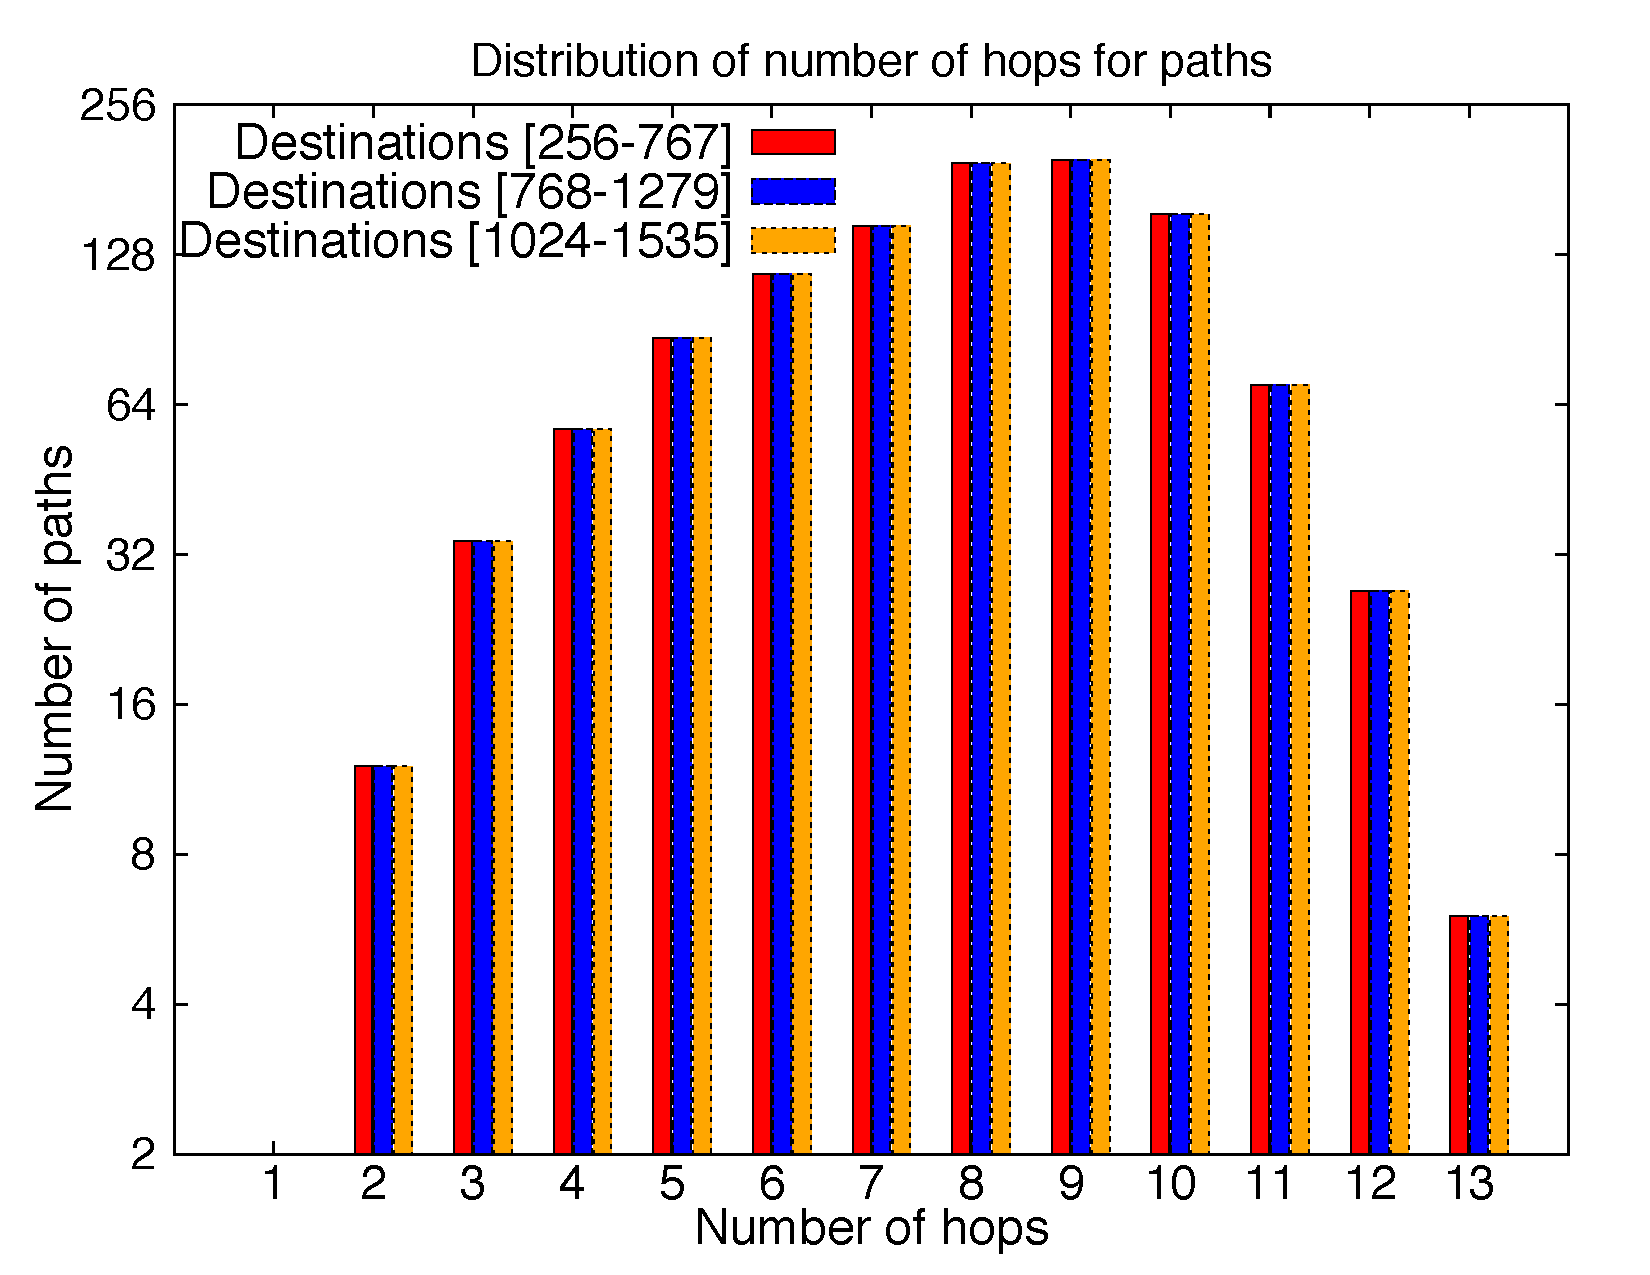
\includegraphics[width=\textwidth]{report_figures/incrdist/2k/hop_histo.pdf}
                \caption{Distribution of number of hops over paths}
                \label{fig:incrdist_2k_hop}
        \end{subfigure}%
        ~ %add desired spacing between images, e. g. ~, \quad, \qquad, \hfill etc.
          %(or a blank line to force the subfigure onto a new line)
        \begin{subfigure}[b]{0.49\textwidth}
                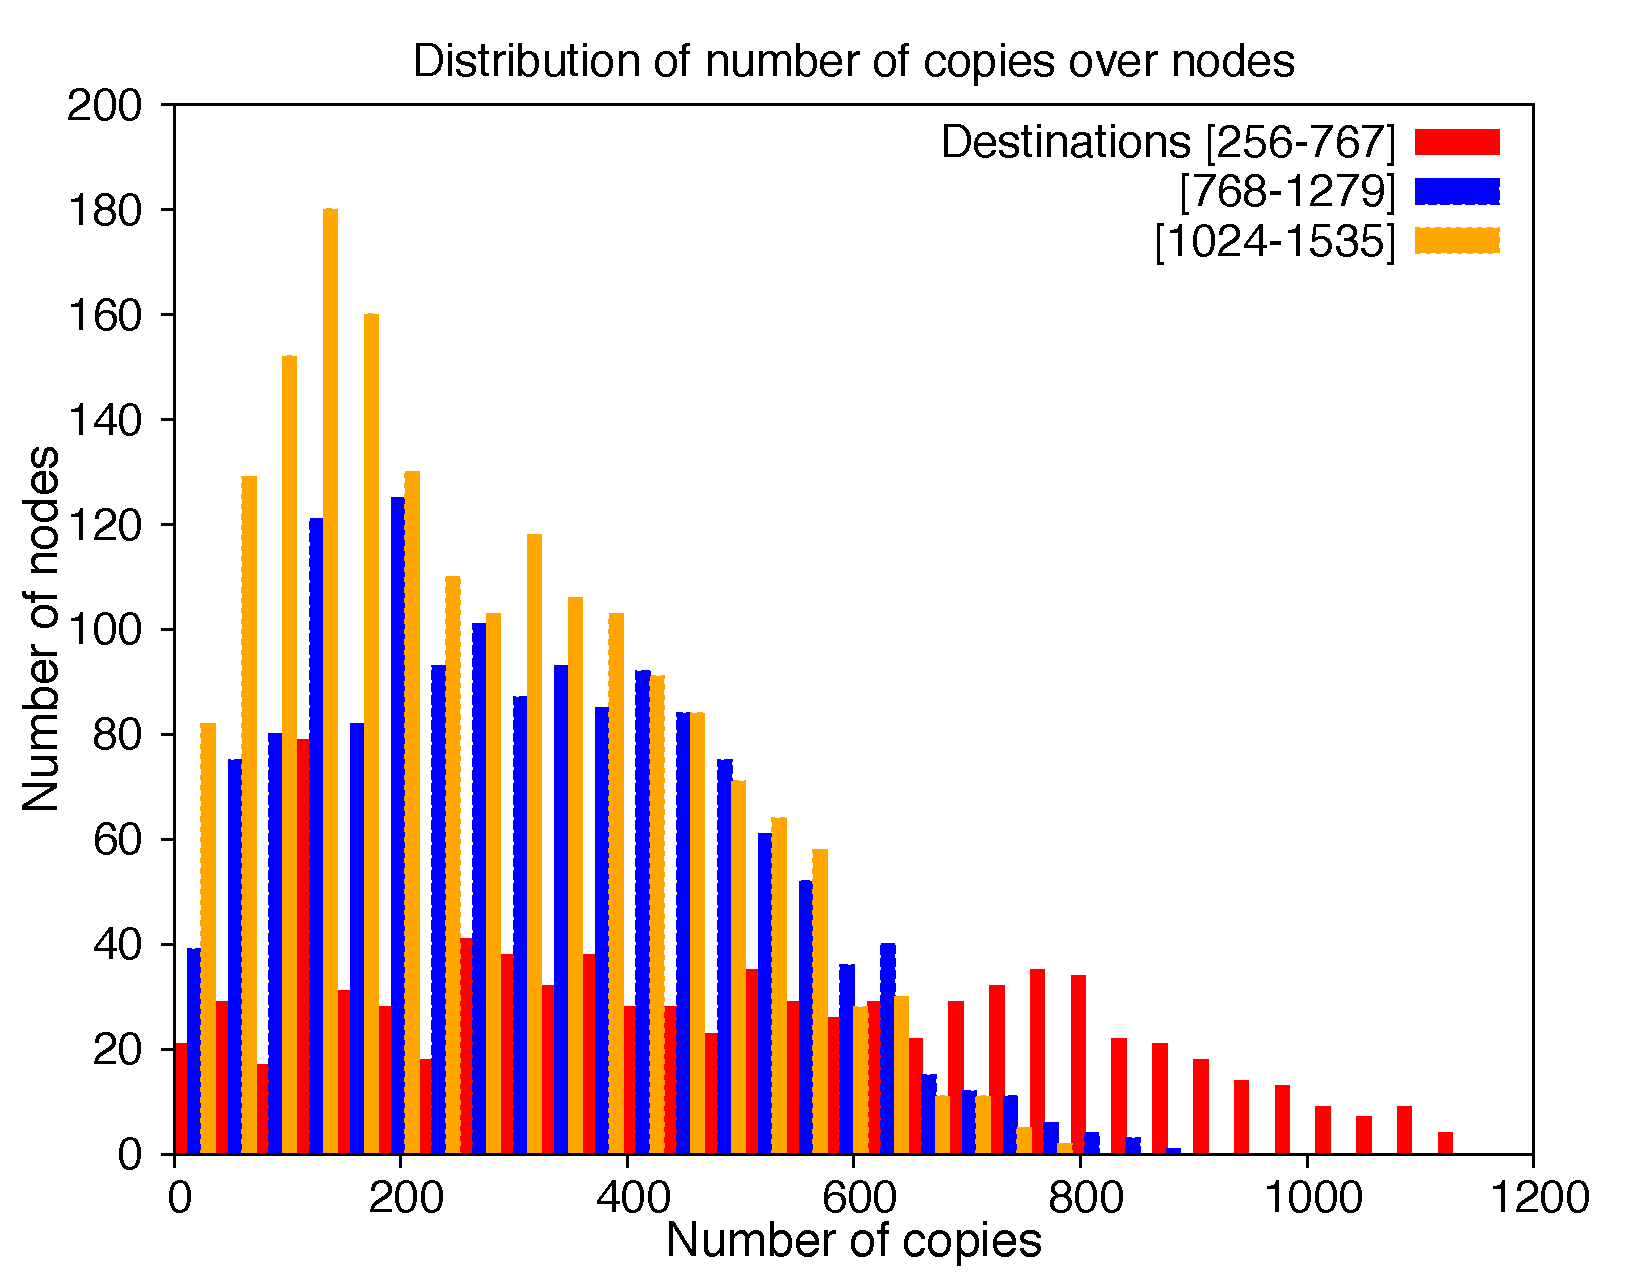
\includegraphics[width=\textwidth]{report_figures/incrdist/2k/copy_histo.pdf}
                \caption{Distribution of number of copies over nodes}
                \label{fig:incrdist_2k_copy}
        \end{subfigure}
        ~ %add desired spacing between images, e. g. ~, \quad, \qquad, \hfill etc.
          %(or a blank line to force the subfigure onto a new line)
        \begin{subfigure}[b]{0.49\textwidth}
                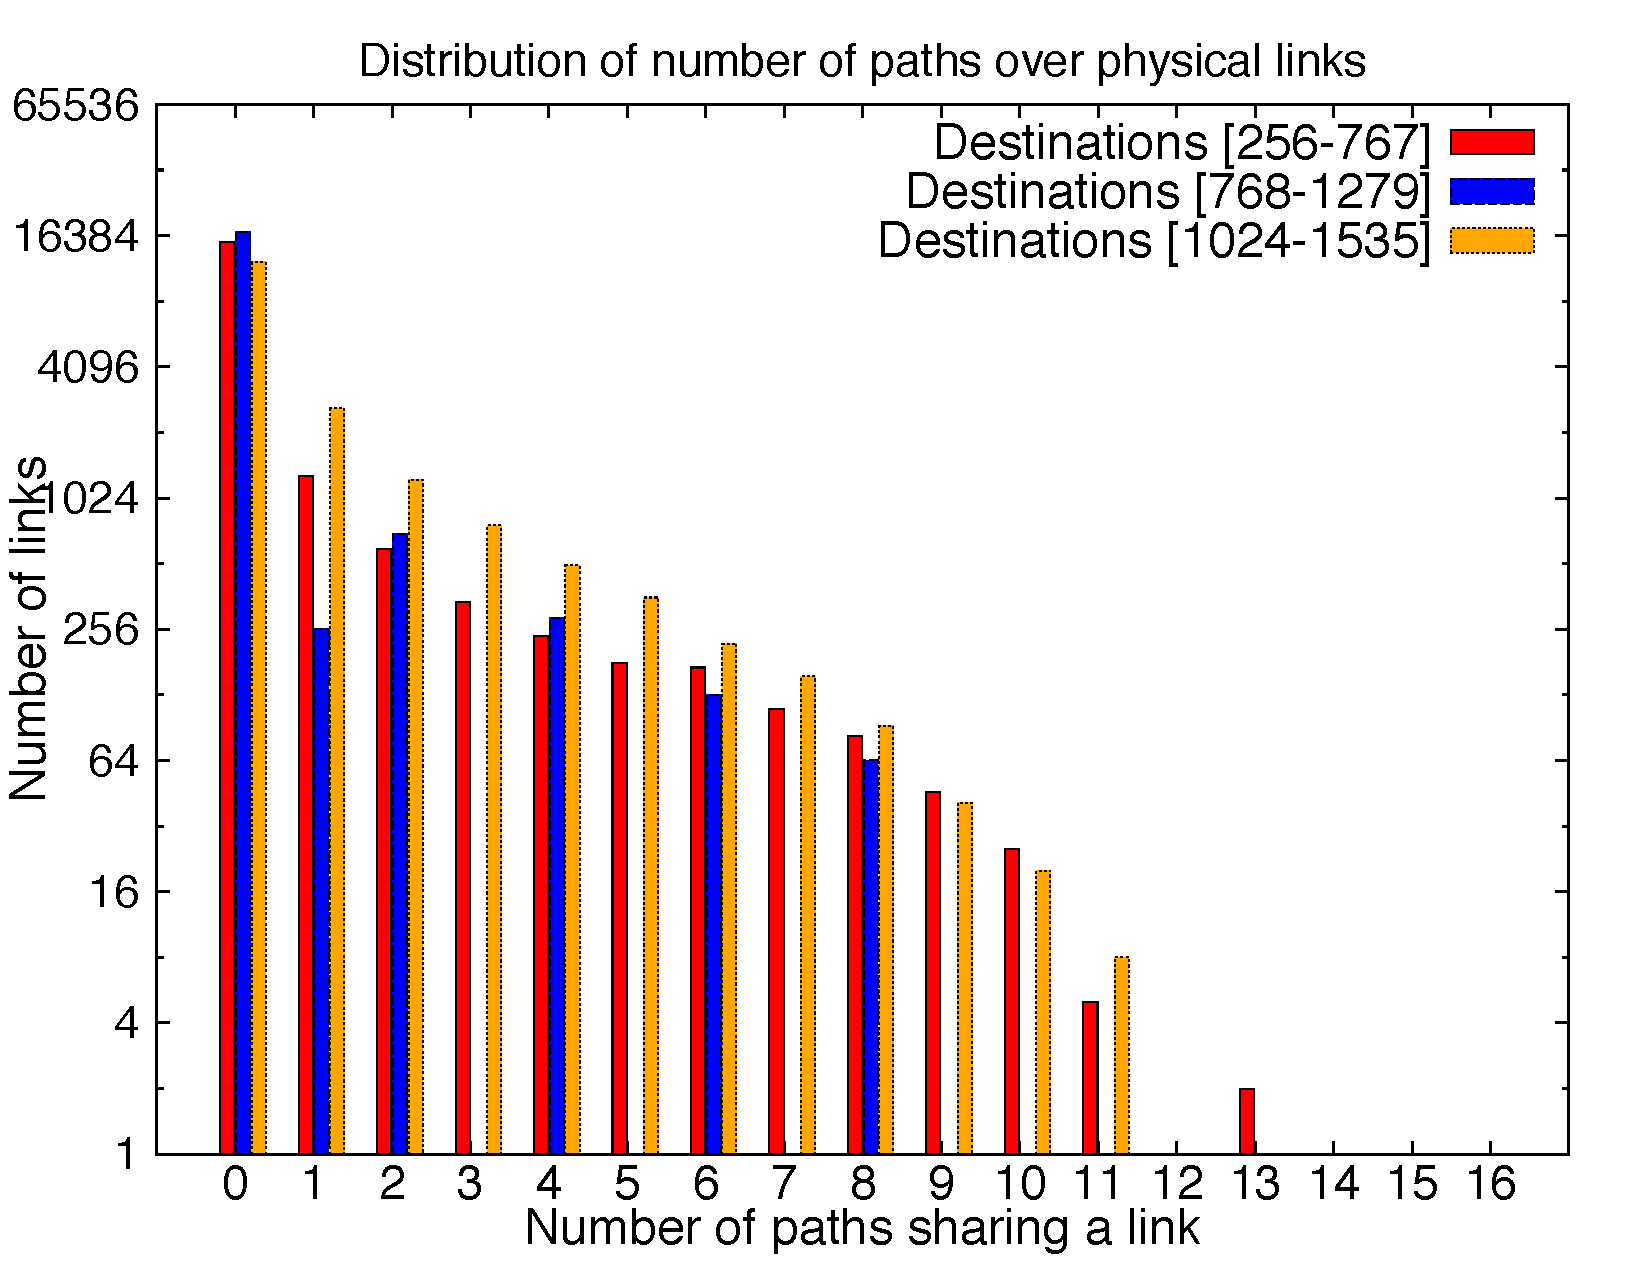
\includegraphics[width=\textwidth]{report_figures/incrdist/2k/loadpath_histo.pdf}
                \caption{Distribution of number of paths over physicallinks}
                \label{fig:incrdist_2k_loadpath}
        \end{subfigure}
        ~ %add desired spacing between images, e. g. ~, \quad, \qquad, \hfill etc.
          %(or a blank line to force the subfigure onto a new line)
        \begin{subfigure}[b]{0.49\textwidth}
                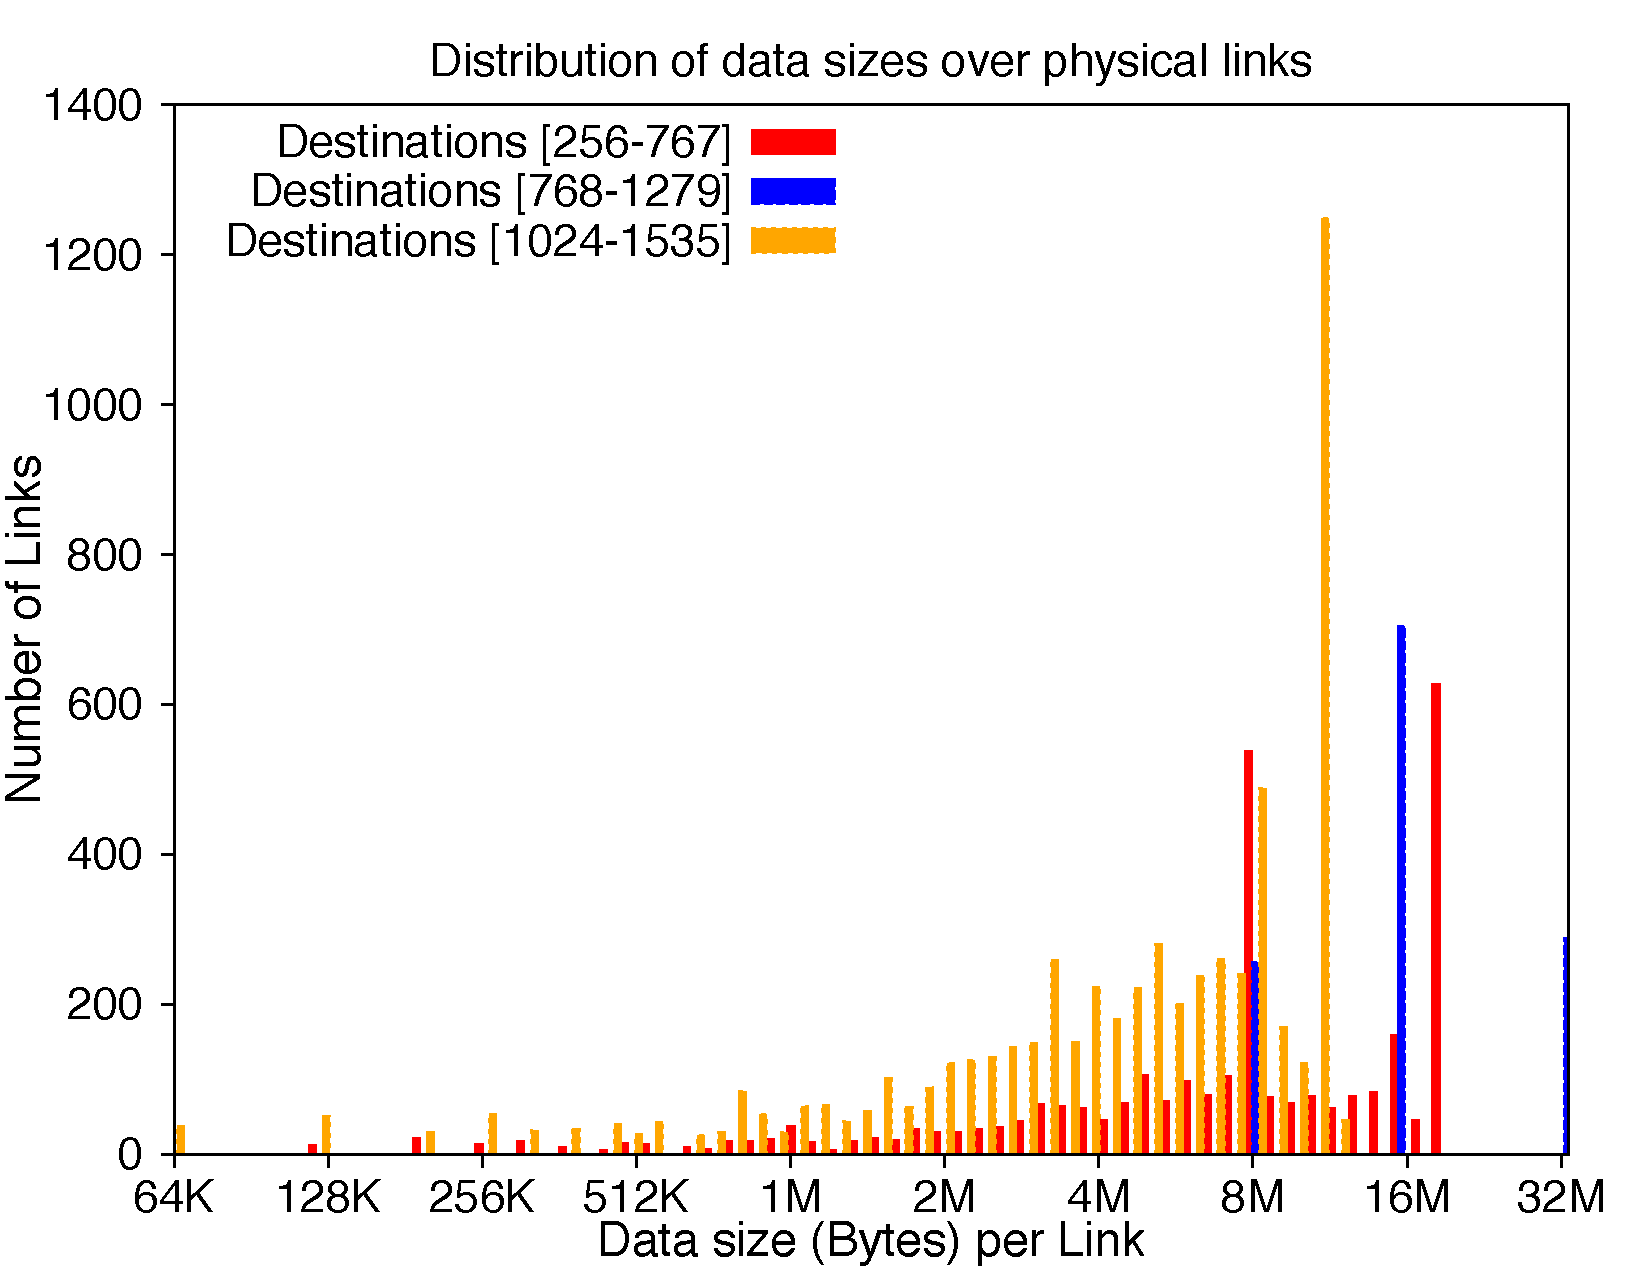
\includegraphics[width=\textwidth]{report_figures/incrdist/2k/loaddata_histo.pdf}
                \caption{Distribution of total data size over physical links}
                \label{fig:incrdist_2k_loaddata}
        \end{subfigure}
        ~ %add desired spacing between images, e. g. ~, \quad, \qquad, \hfill etc.
          %(or a blank line to force the subfigure onto a new line)
        \begin{subfigure}[b]{0.49\textwidth}
                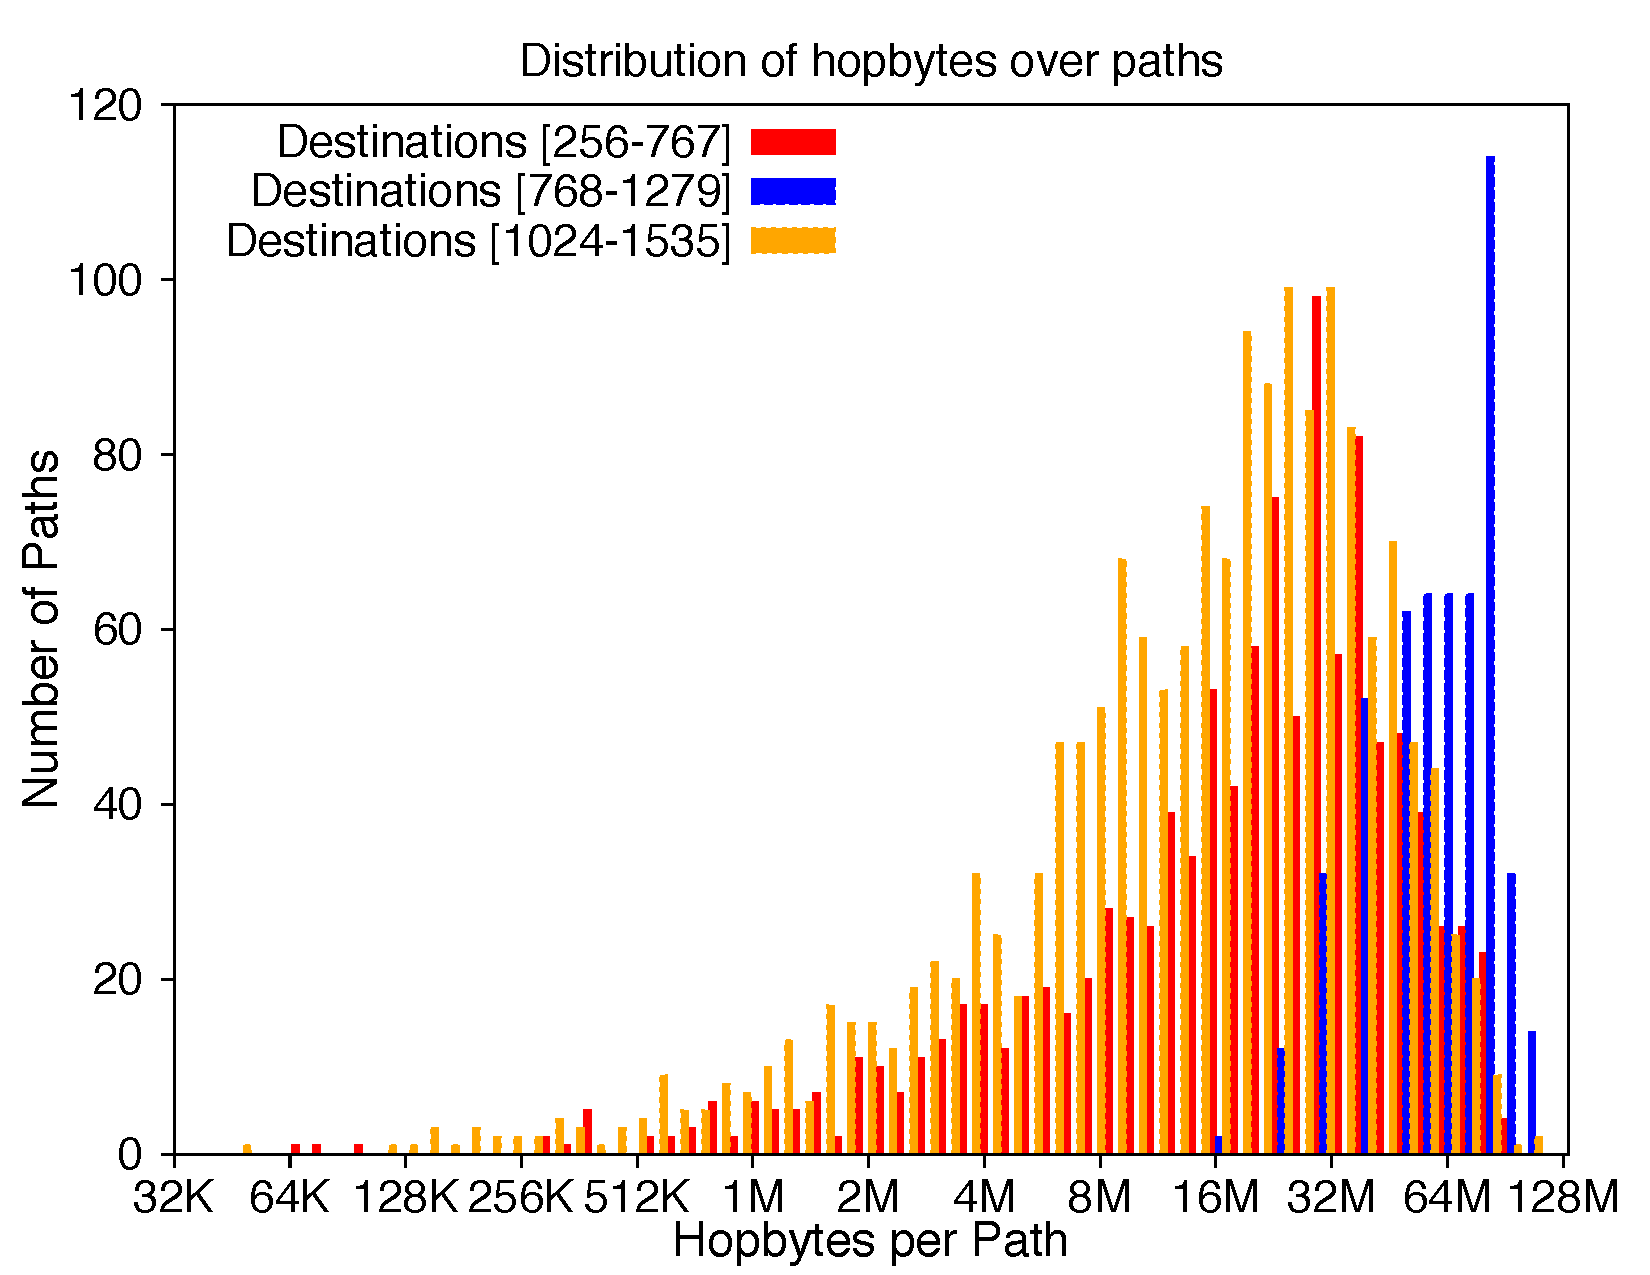
\includegraphics[width=\textwidth]{report_figures/incrdist/2k/hopbyte_histo.pdf}
                \caption{Distribution of hopbytes over paths}
                \label{fig:incrdist_2k_hopbyte}
        \end{subfigure}
        ~ %add desired spacing between images, e. g. ~, \quad, \qquad, \hfill etc.
          %(or a blank line to force the subfigure onto a new line)
        \begin{subfigure}[b]{0.49\textwidth}
                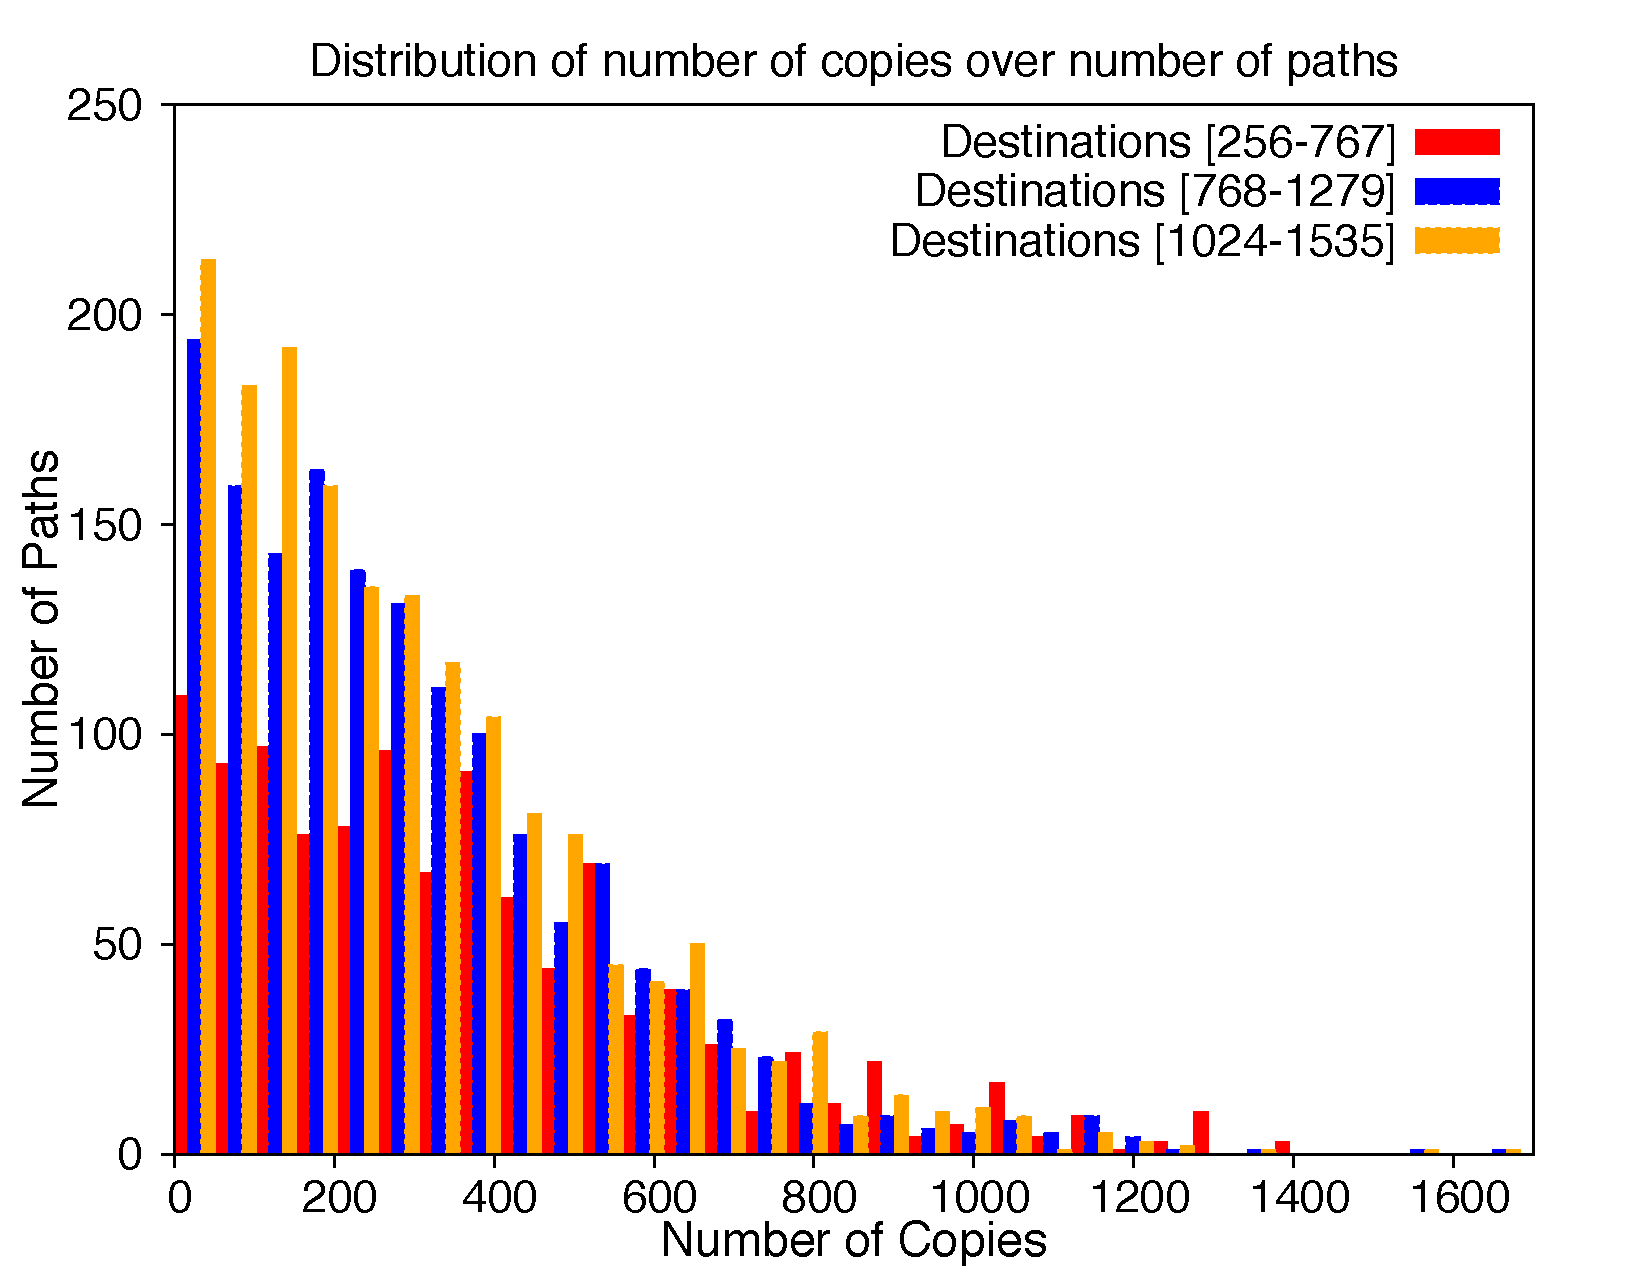
\includegraphics[width=\textwidth]{report_figures/incrdist/2k/hopcopy_histo.pdf}
                \caption{Distribution of number of copies over paths}
                \label{fig:incrdist_2k_hopcopy}
        \end{subfigure}
        \caption{Historgram of hops, copies, load in terms of number of paths and data size - 2K nodes}
        \label{fig:incrdist_2k_histo}
\end{figure}

\clearpage
\newpage

\section {Increasing destination sizes}

\subsection{Total nodes of 2048}

Number of sources is 64. Number of destinations increases from 128, 256, 512, 1024. 

\begin{figure}[h]
\vspace{-0.1in}
\centering
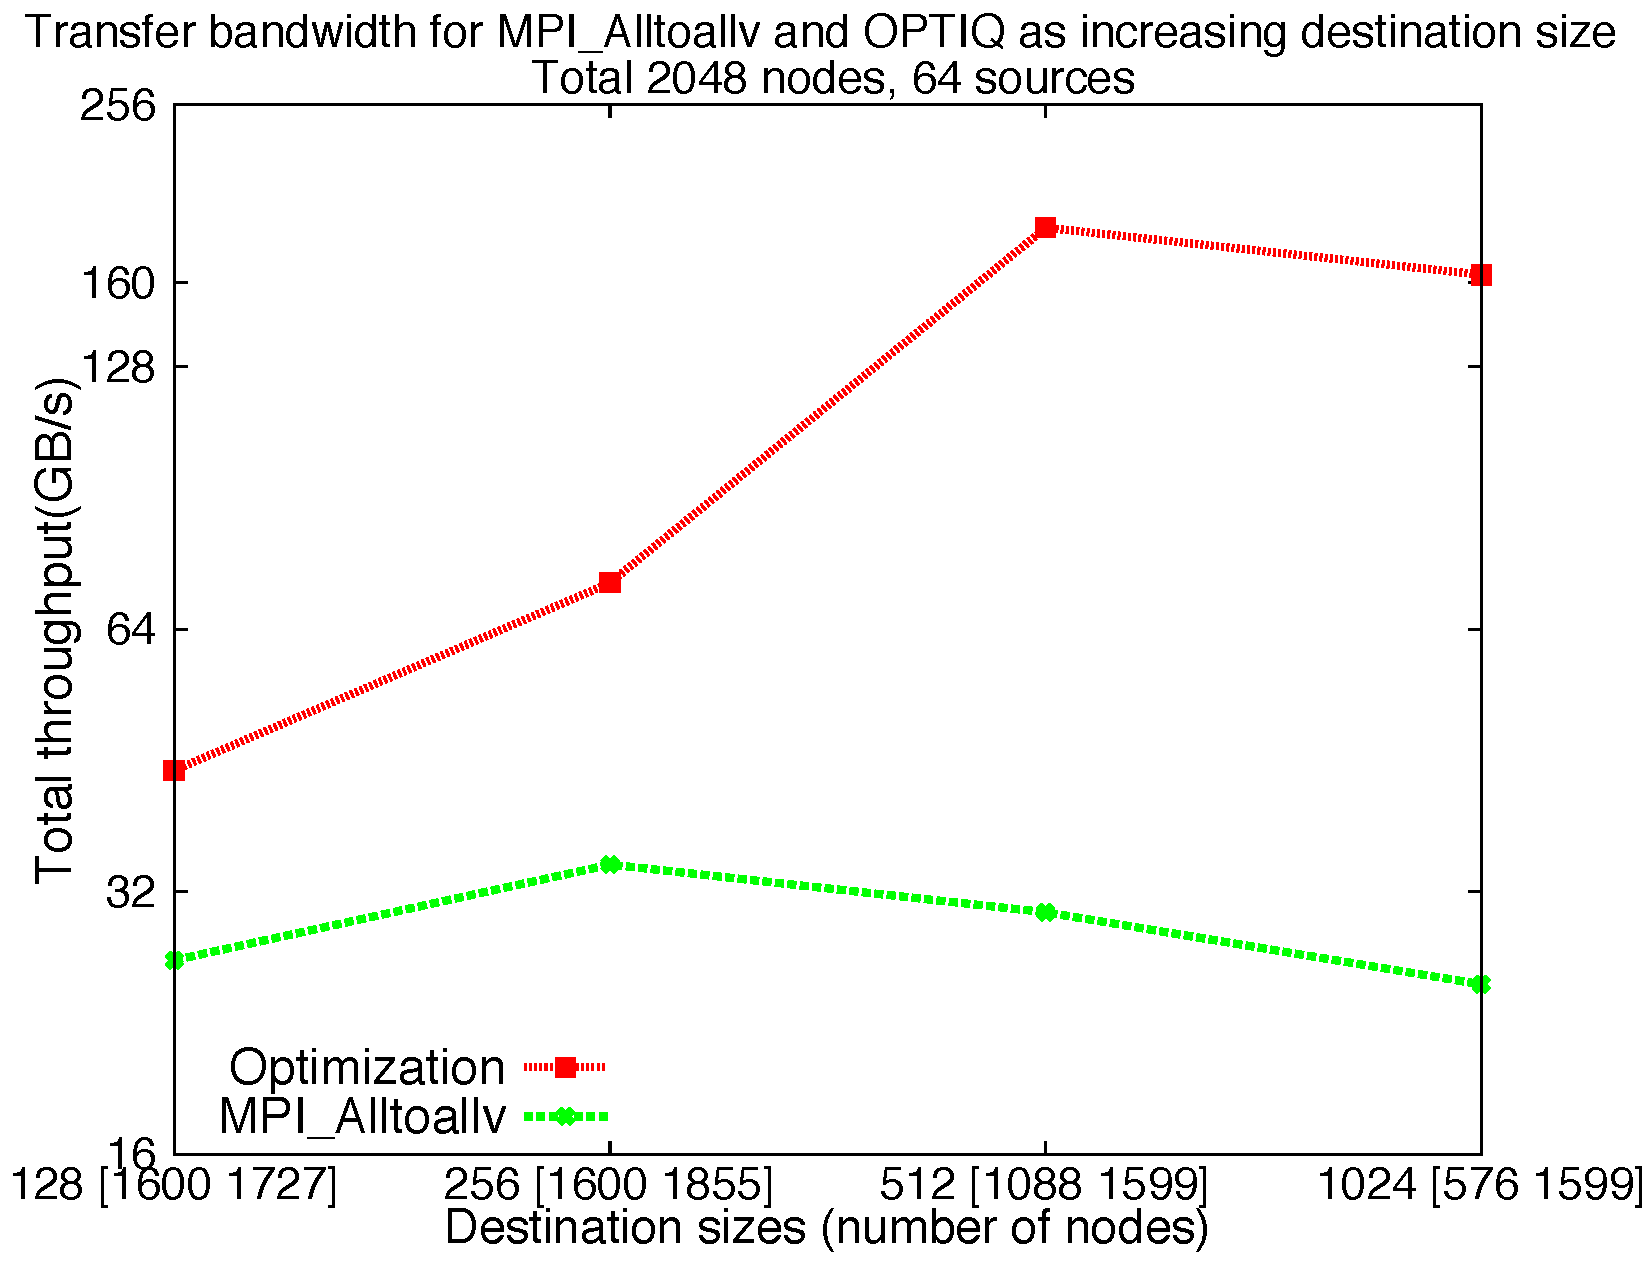
\includegraphics[scale=0.40]{report_figures/incrsize/incrsize_2k.pdf}
\vspace{-0.1in}
\caption{Increasing Destination Sizes}
\vspace{-0.1in}
\label{fig:incrsize_2k}
\end{figure}

\section{Multiple ranks}

\section{Multiple message sizes}

\section{Chunk size}

\section{Paths selection}

\subsection{Max load varation in selecting paths for Heuristics}

\subsection{Number of paths variation to feed to optimization model}

\end{document}
